% !TeX root = ../hw4.tex
\section{Reproducing the Book's Fractal Plants}

\subsection{Statement}
Use bracketed OL-systems to reproduce each of the plant-like fractals in Figure 7.24 of the book.

Experiment with the production rules and produce at least ten derivatives.

\subsection{Results}\label{sec:p2-results}
Our reproductions for each of the figures in the book are shown below.
Due to the nature of the L-system, each tree is sized quite differently.
This, and the difficulty of reproducibly rendering the scenes in Blender, have the unfortunate consequence of scaling each tree with different aspect ratios, and at different sizes.

\begin{figure}[H]
    \centering
    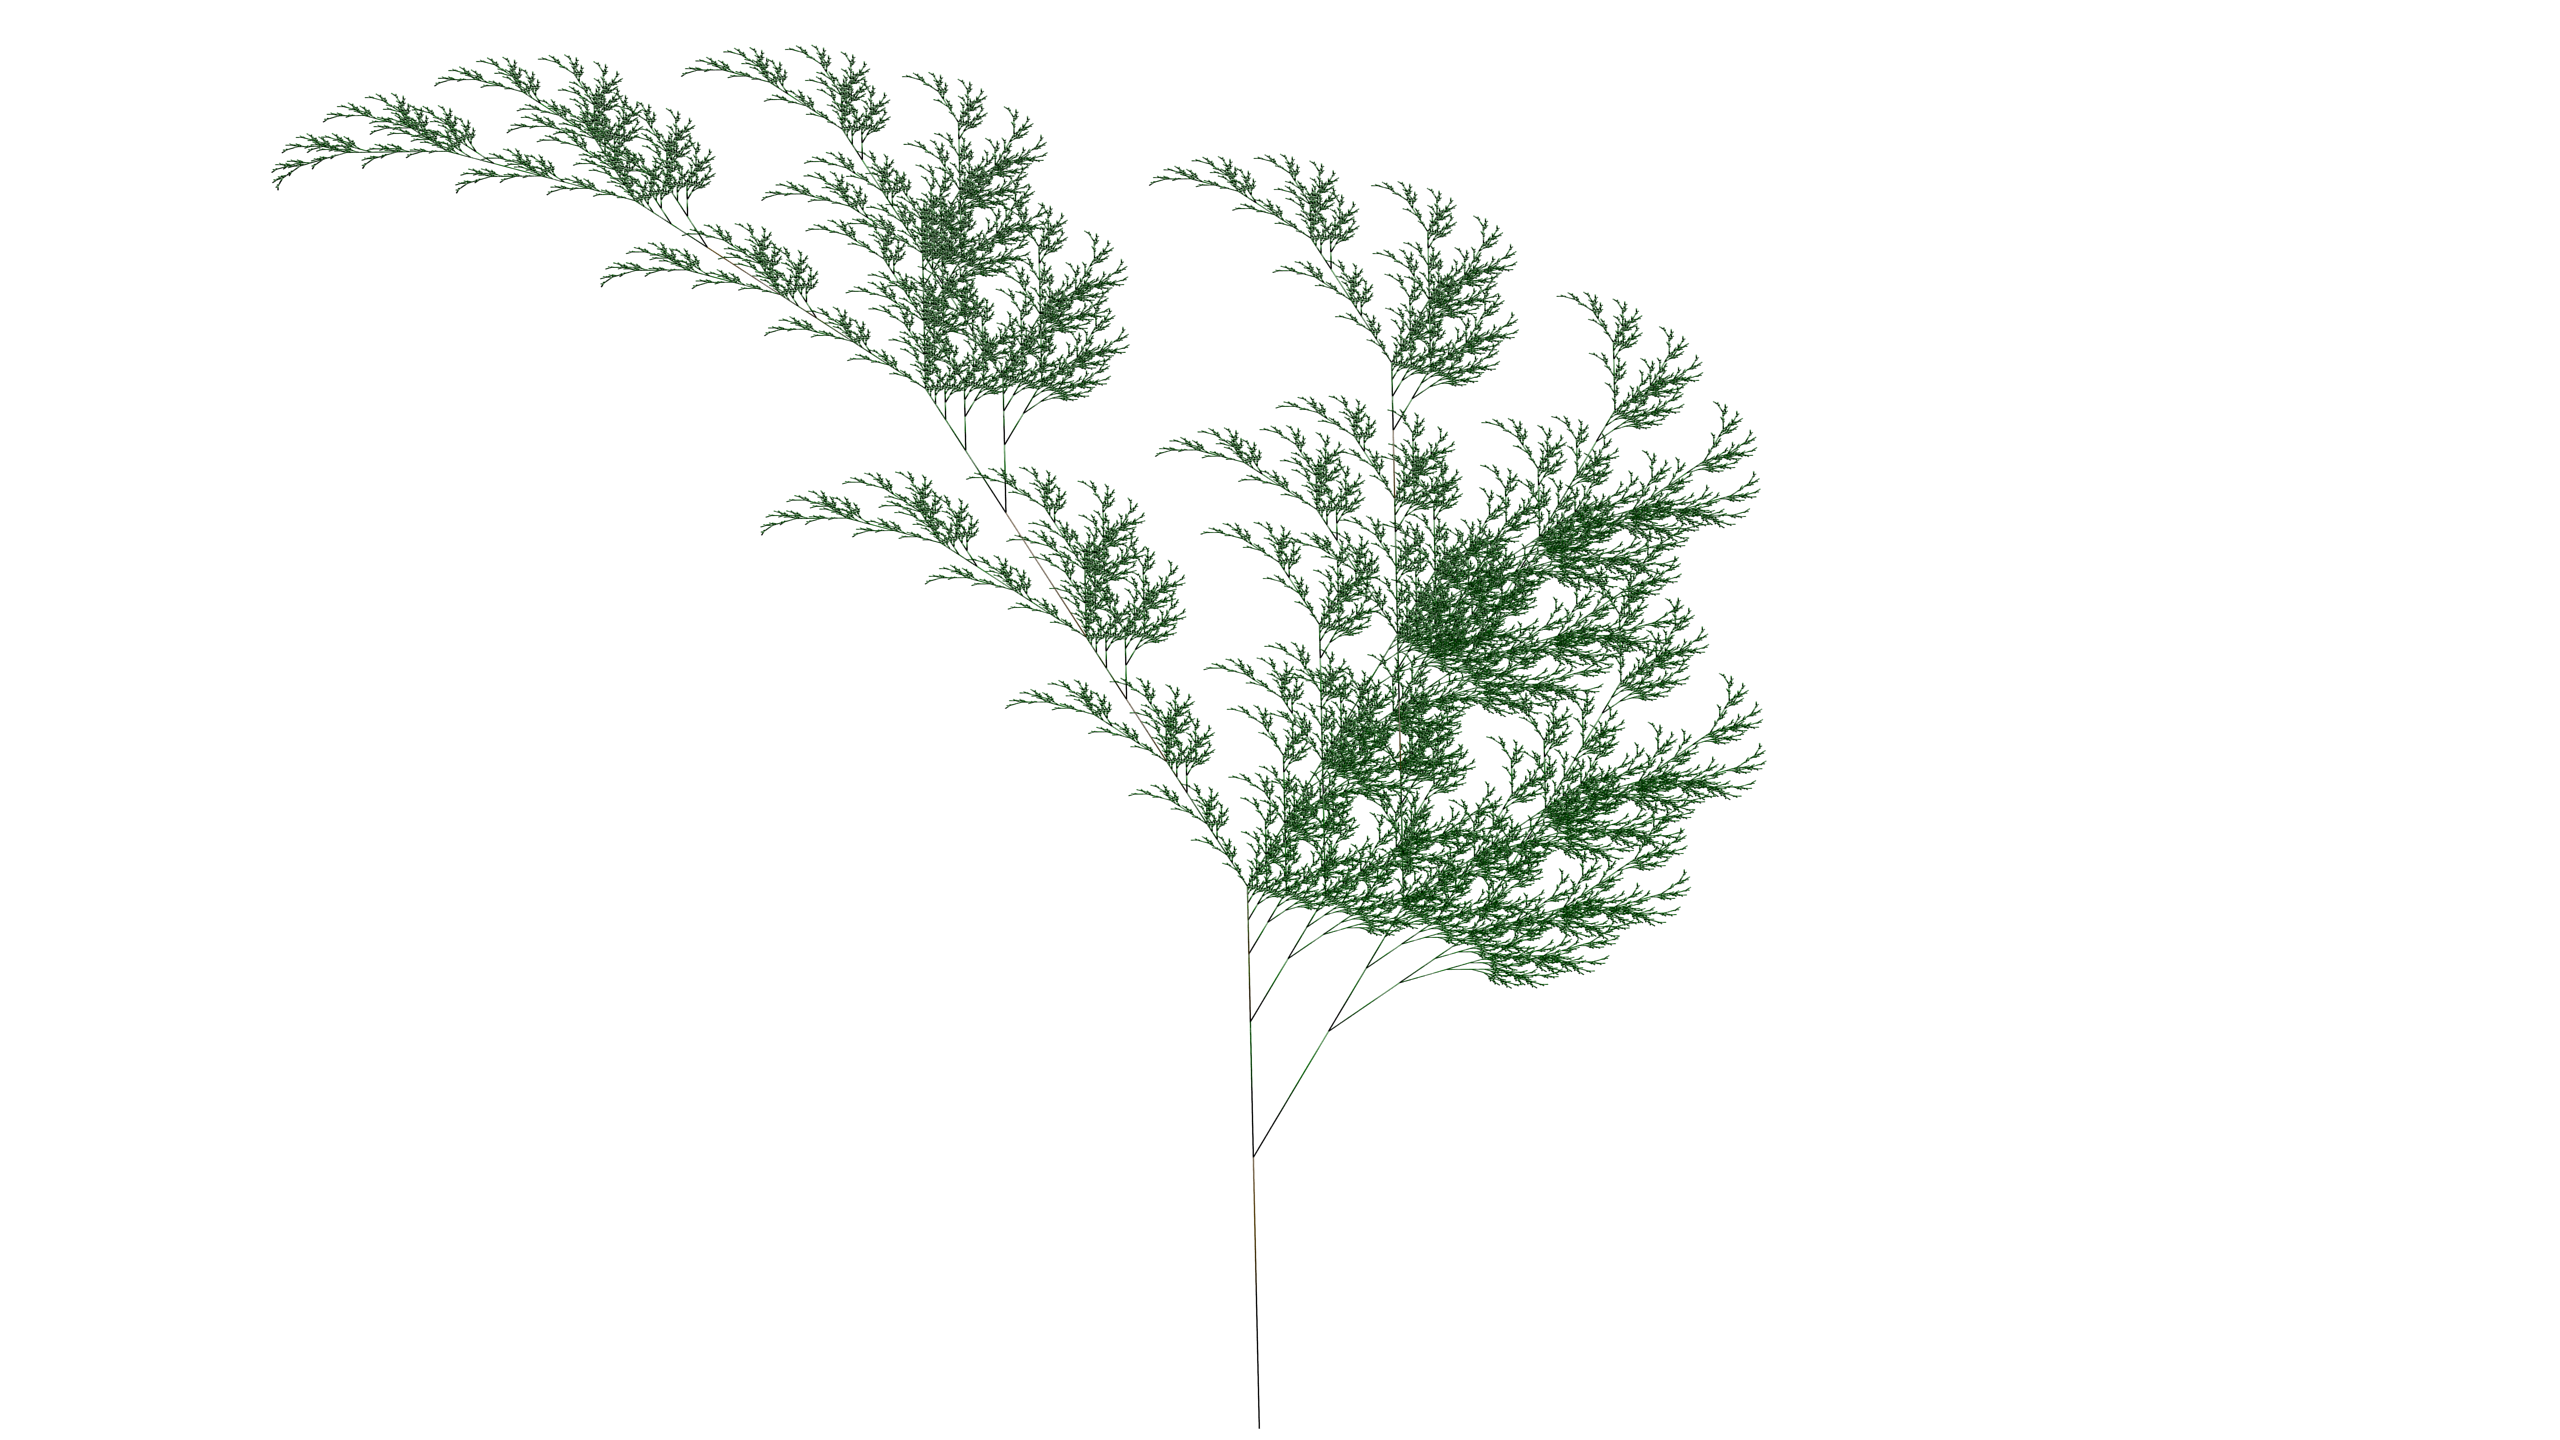
\includegraphics[width=0.90\textwidth]{figures/L-systems/a.png}
    \caption{Problem 2a}\label{fig:prob2a}
\end{figure}

\begin{figure}[H]
    \centering
    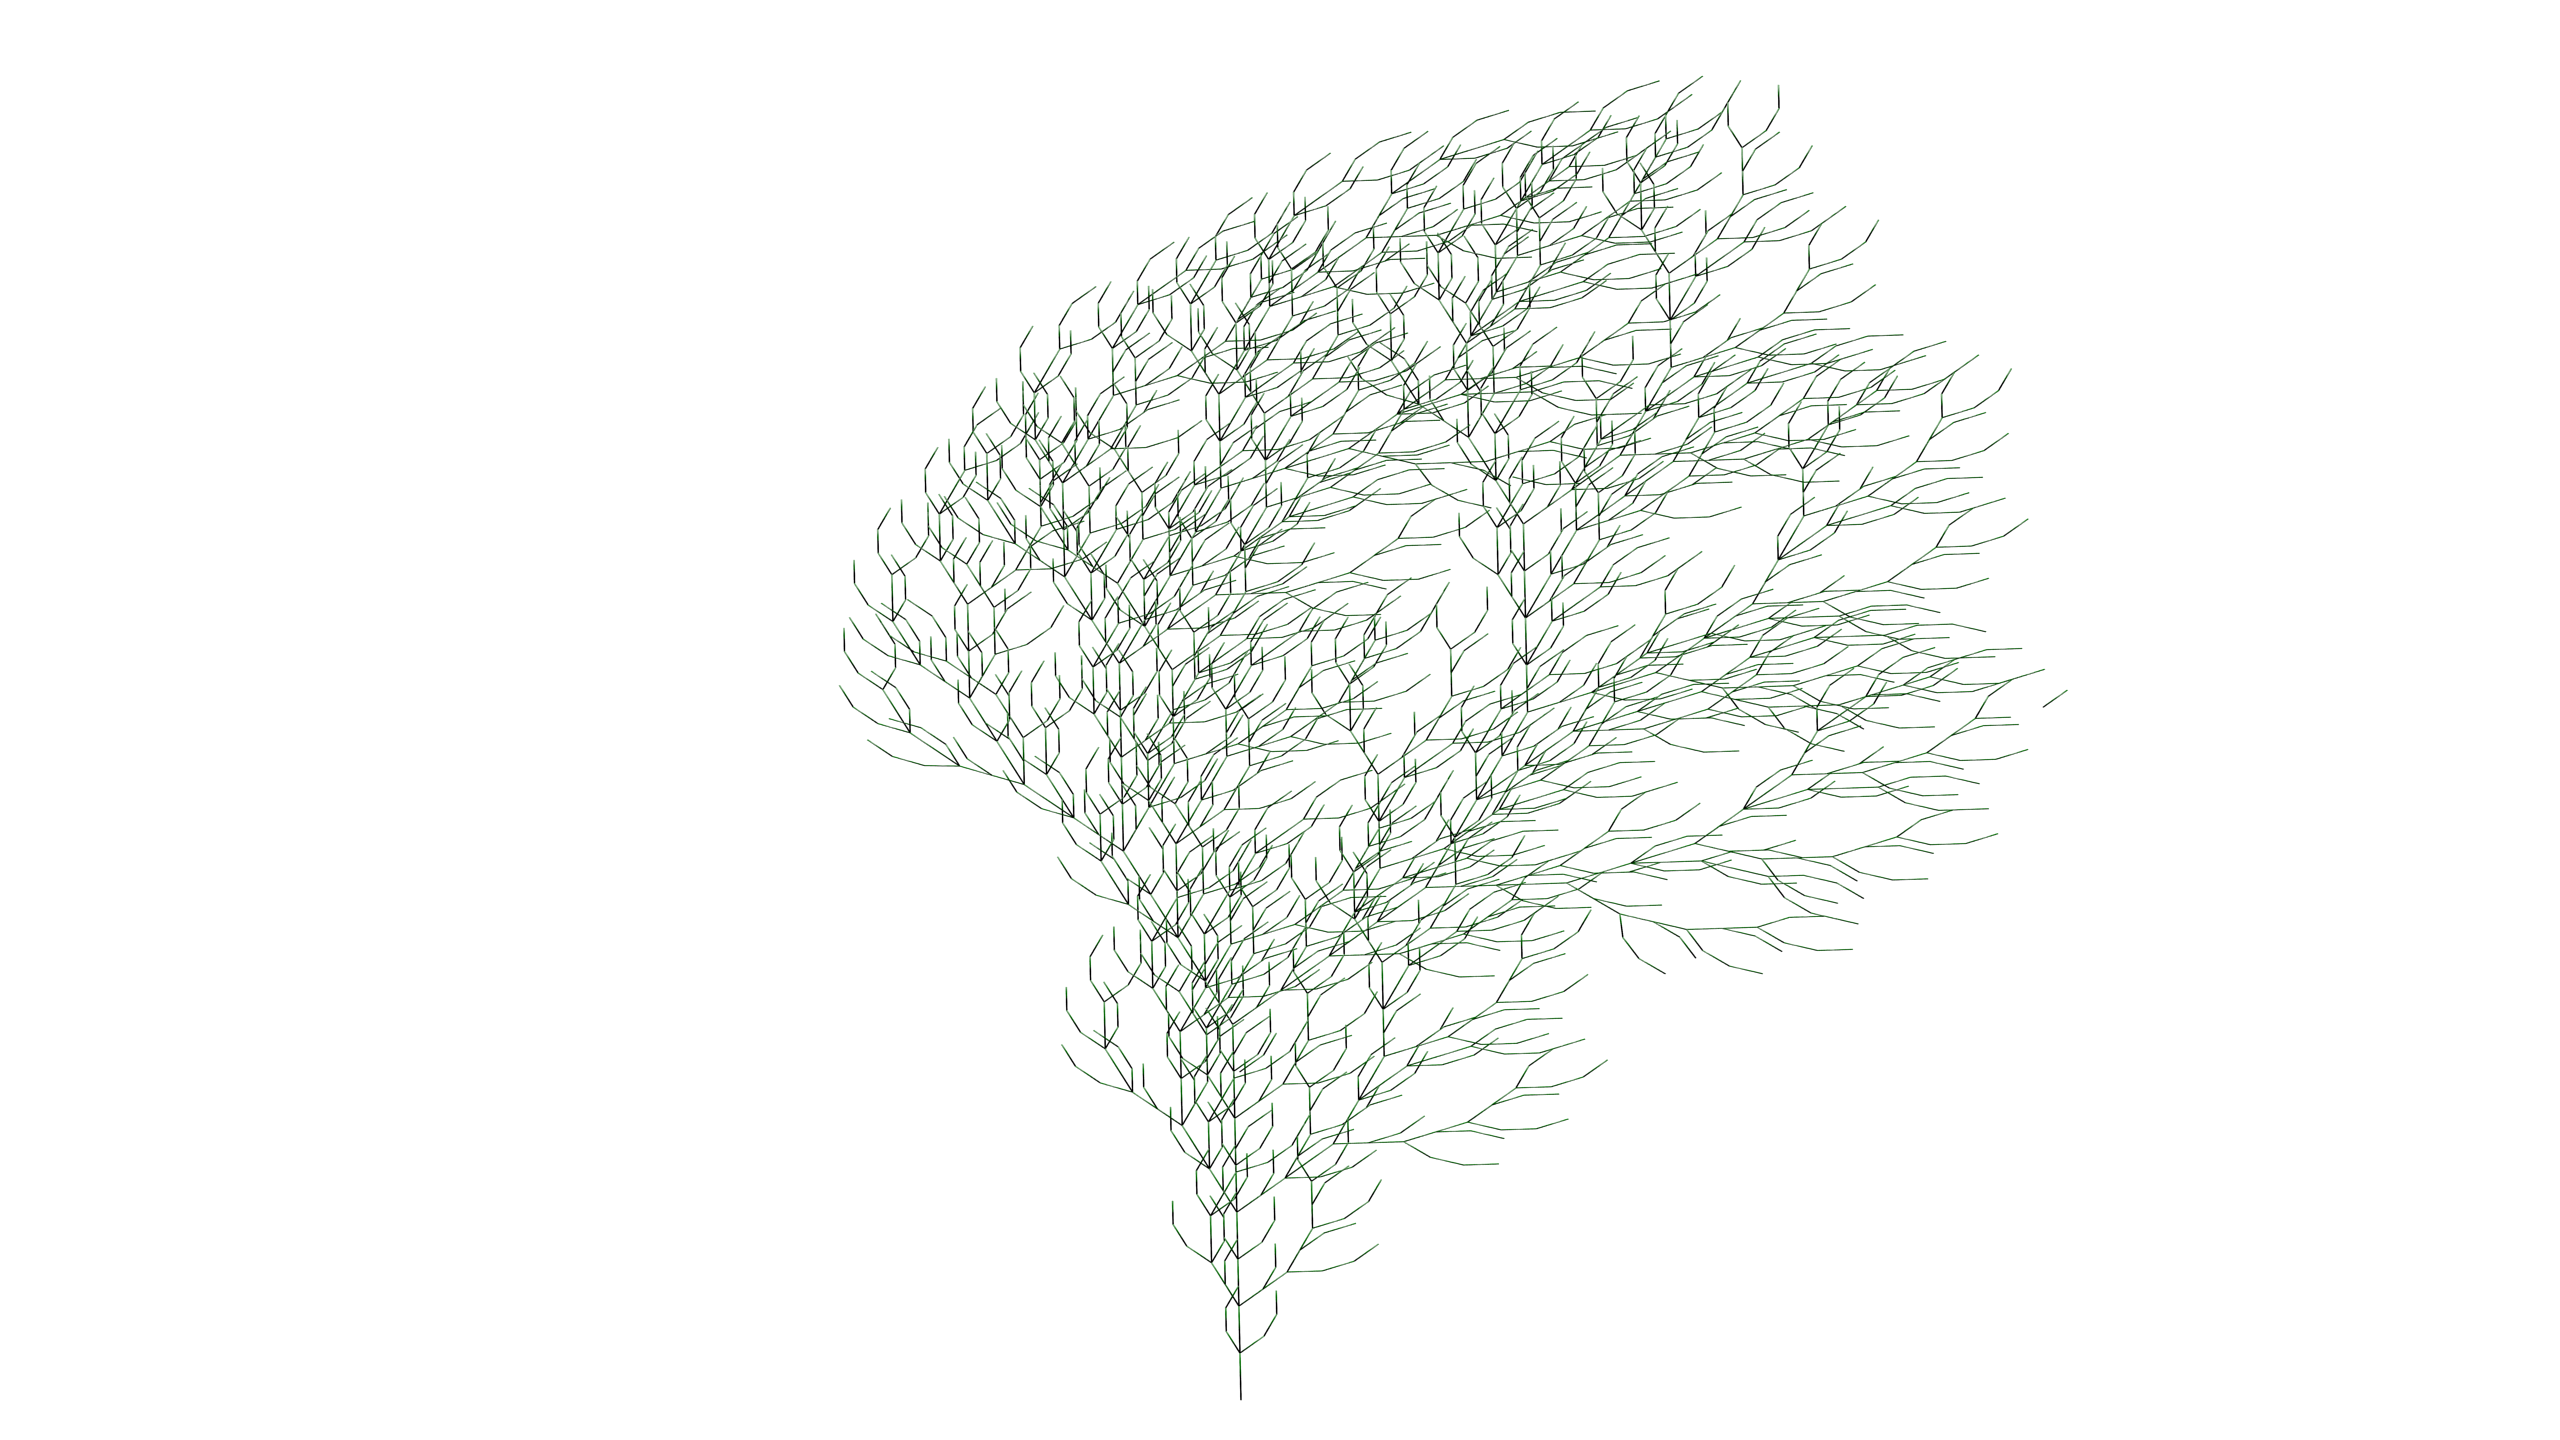
\includegraphics[width=0.90\textwidth]{figures/L-systems/b.png}
    \caption{Problem 2b}\label{fig:prob2b}
\end{figure}

\begin{figure}[H]
    \centering
    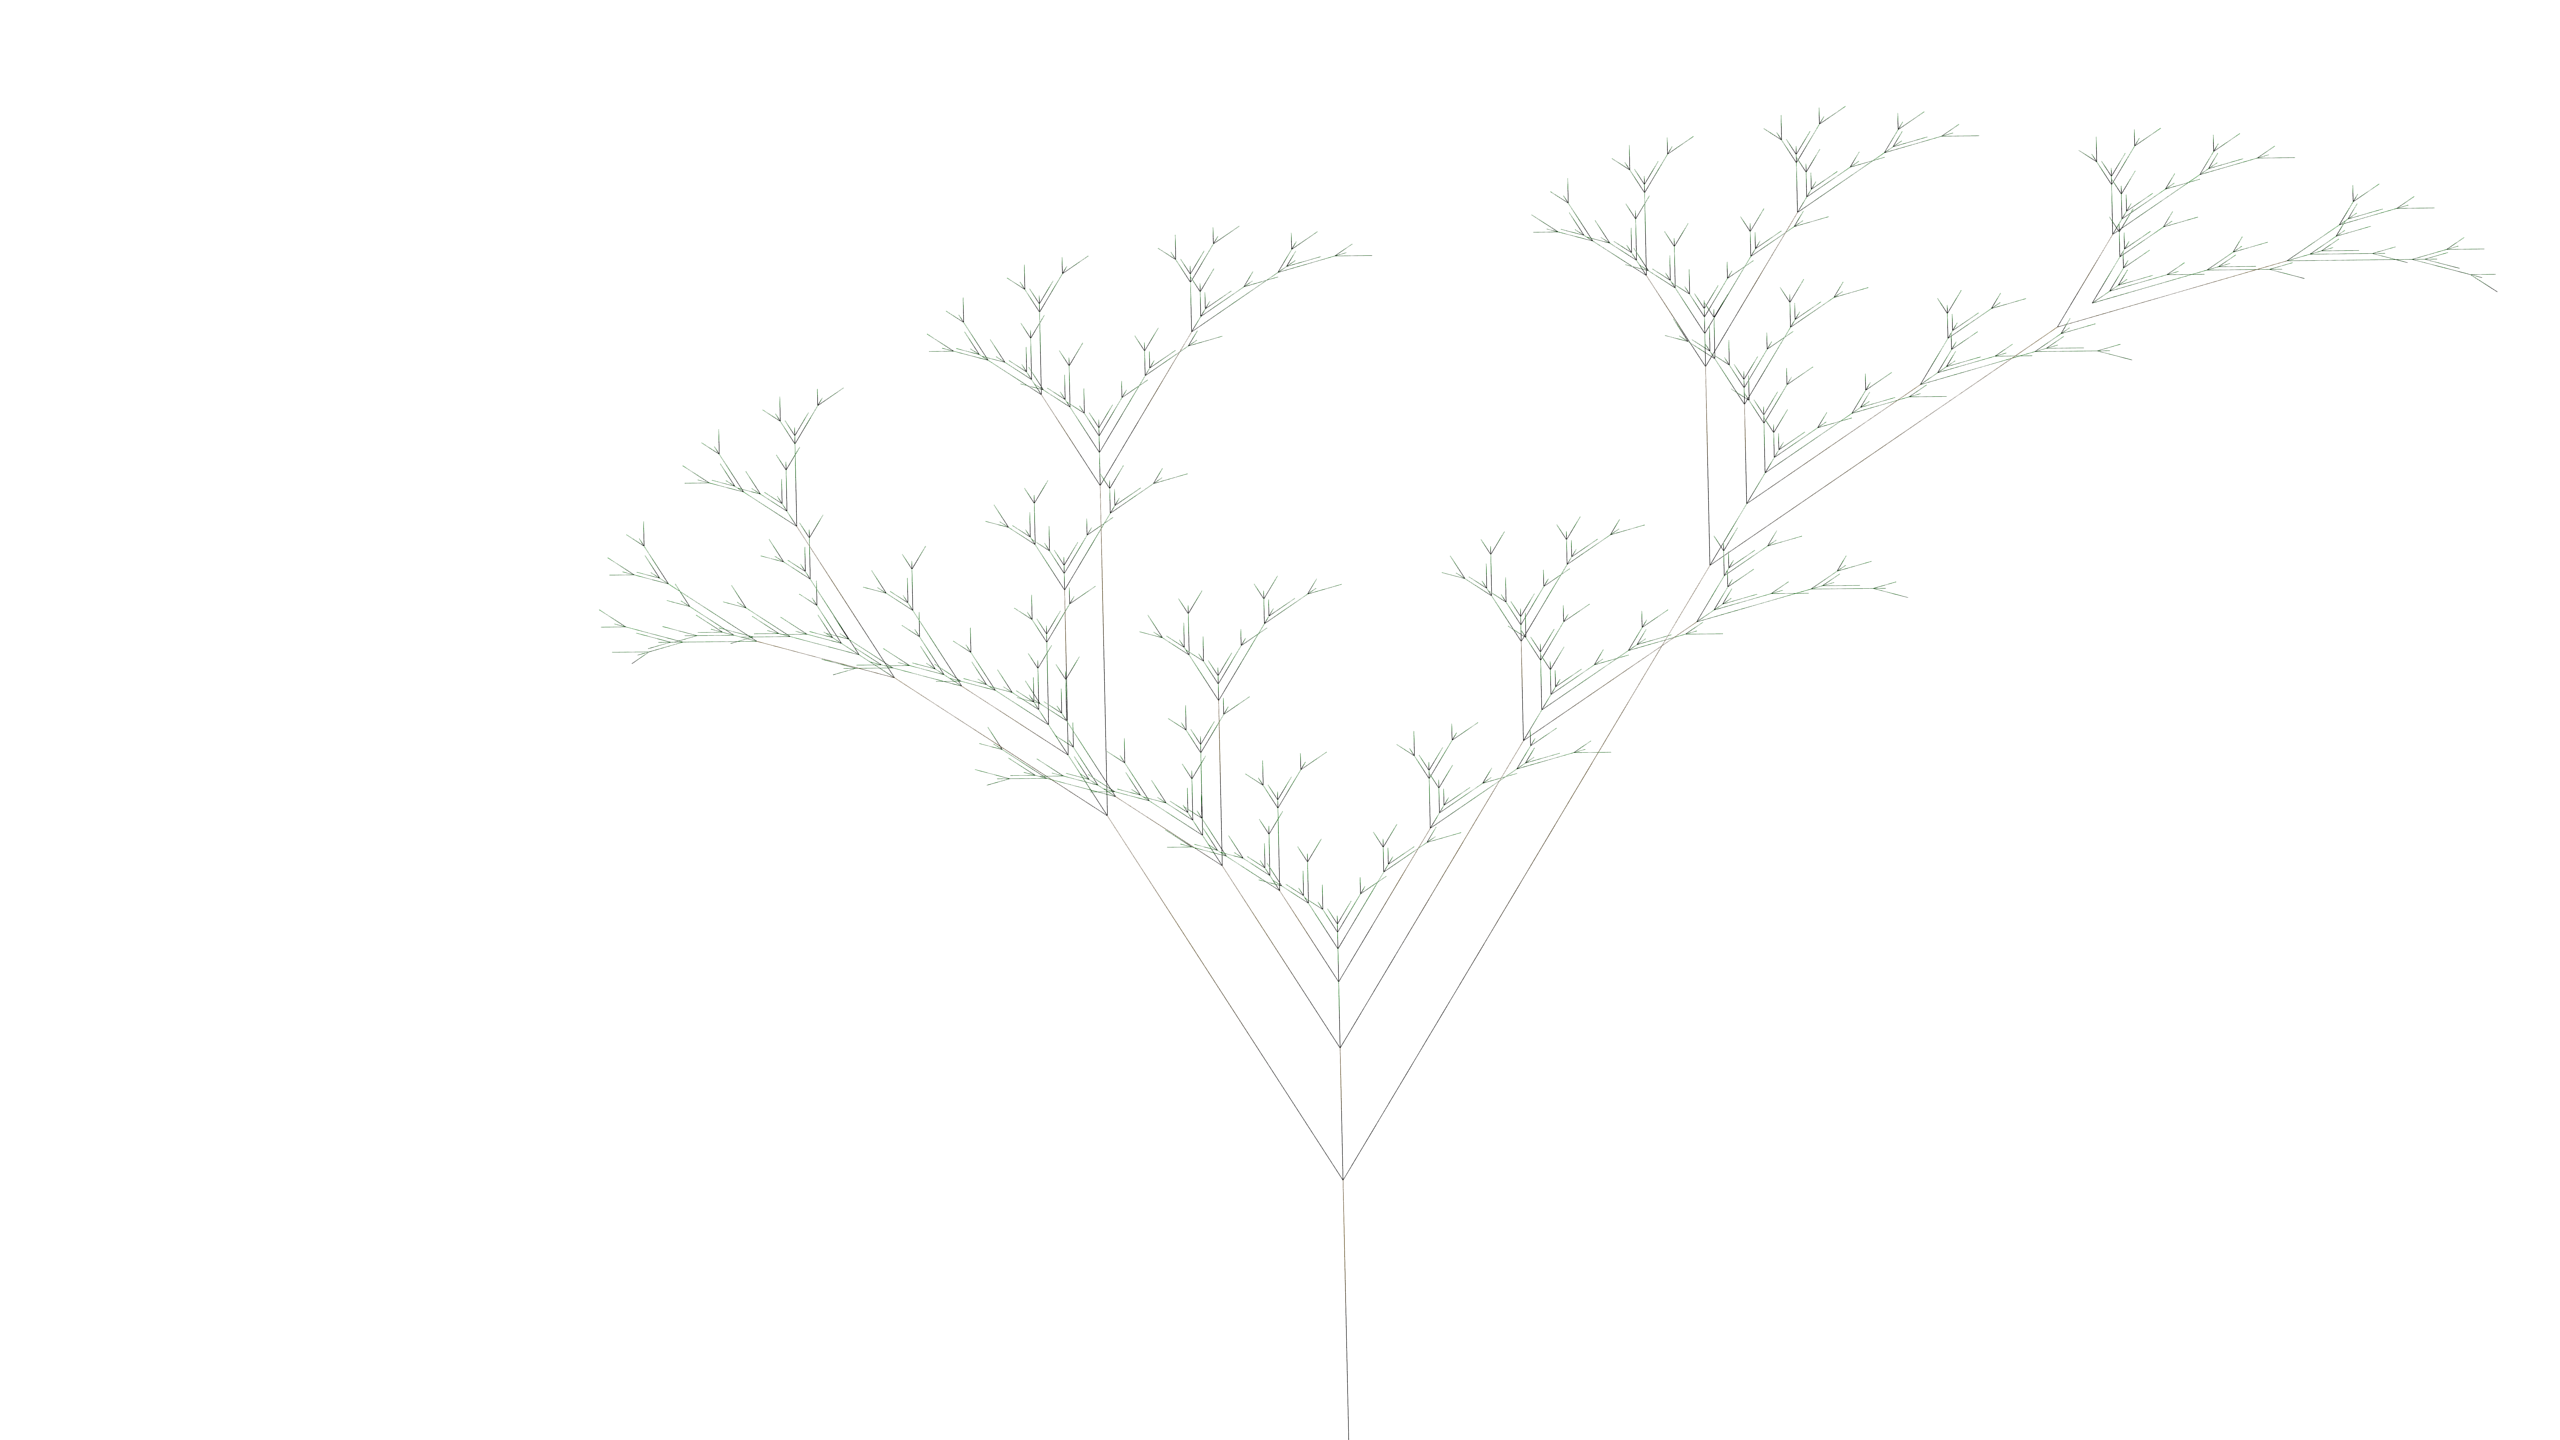
\includegraphics[width=0.90\textwidth]{figures/L-systems/c.png}
    \caption{Problem 2c}\label{fig:prob2c}
\end{figure}

\begin{figure}[H]
    \centering
    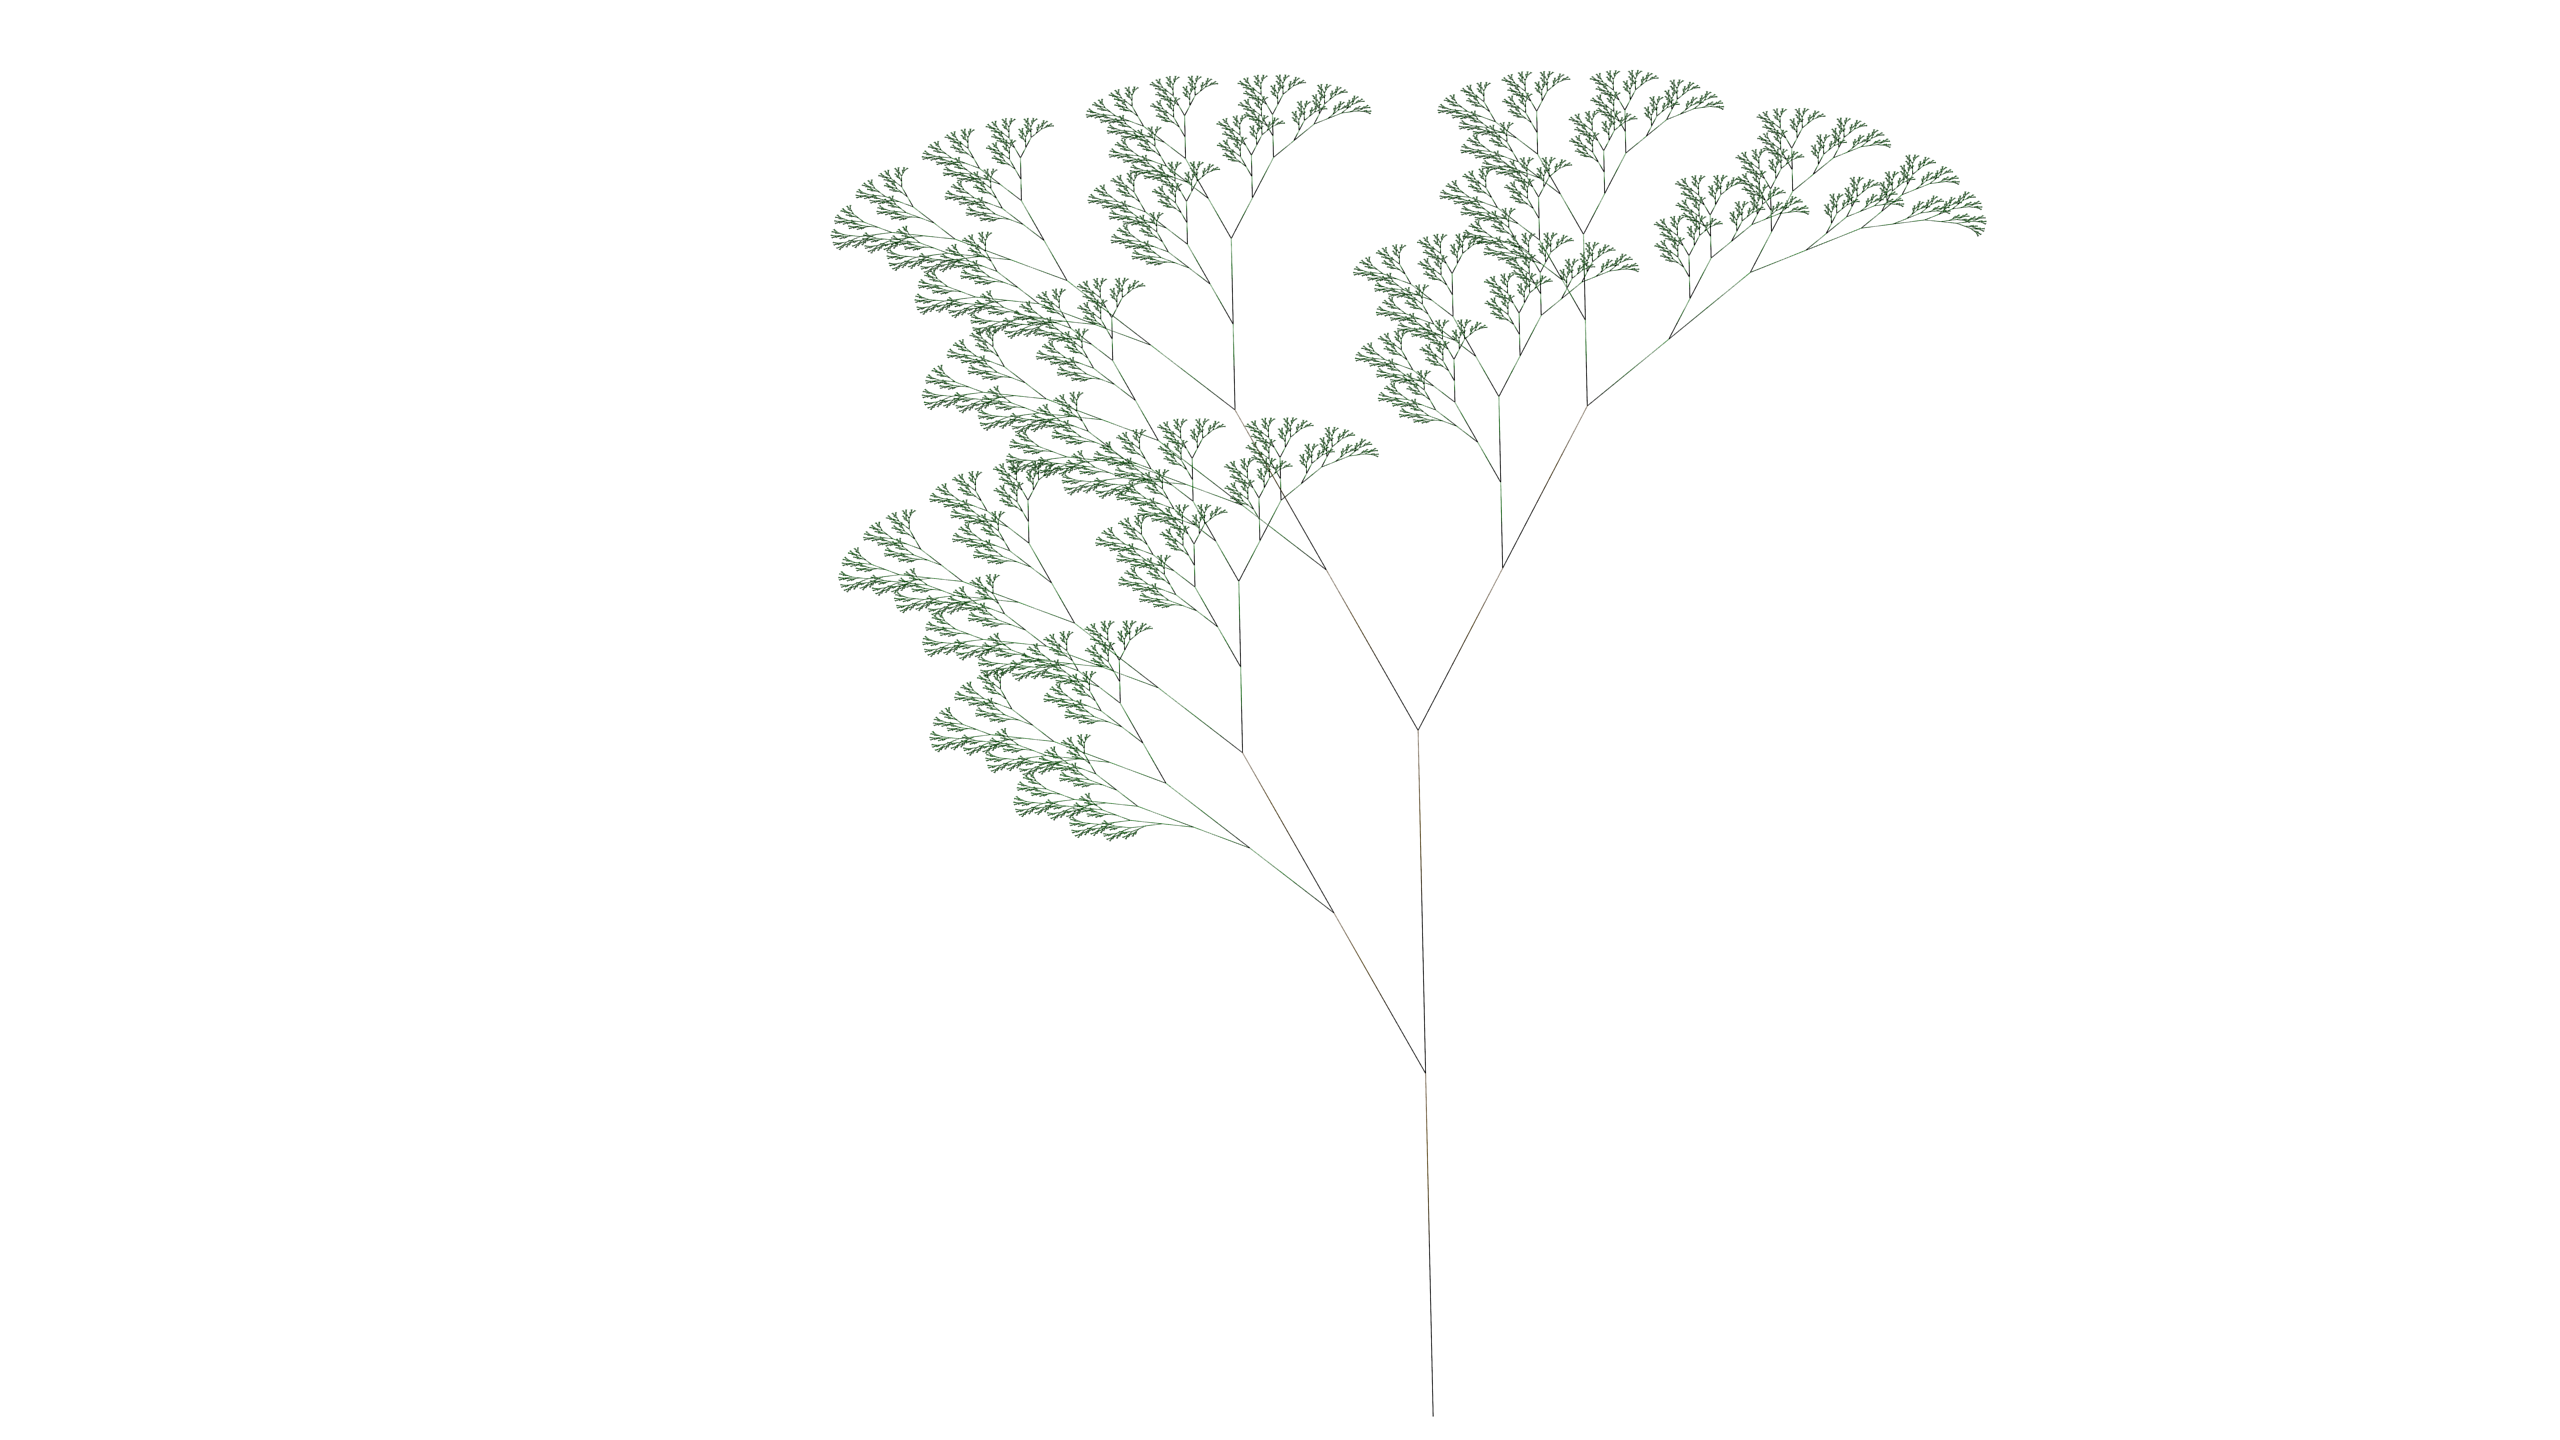
\includegraphics[width=0.90\textwidth]{figures/L-systems/d.png}
    \caption{Problem 2d}\label{fig:prob2d}
\end{figure}

\begin{figure}[H]
    \centering
    \noindent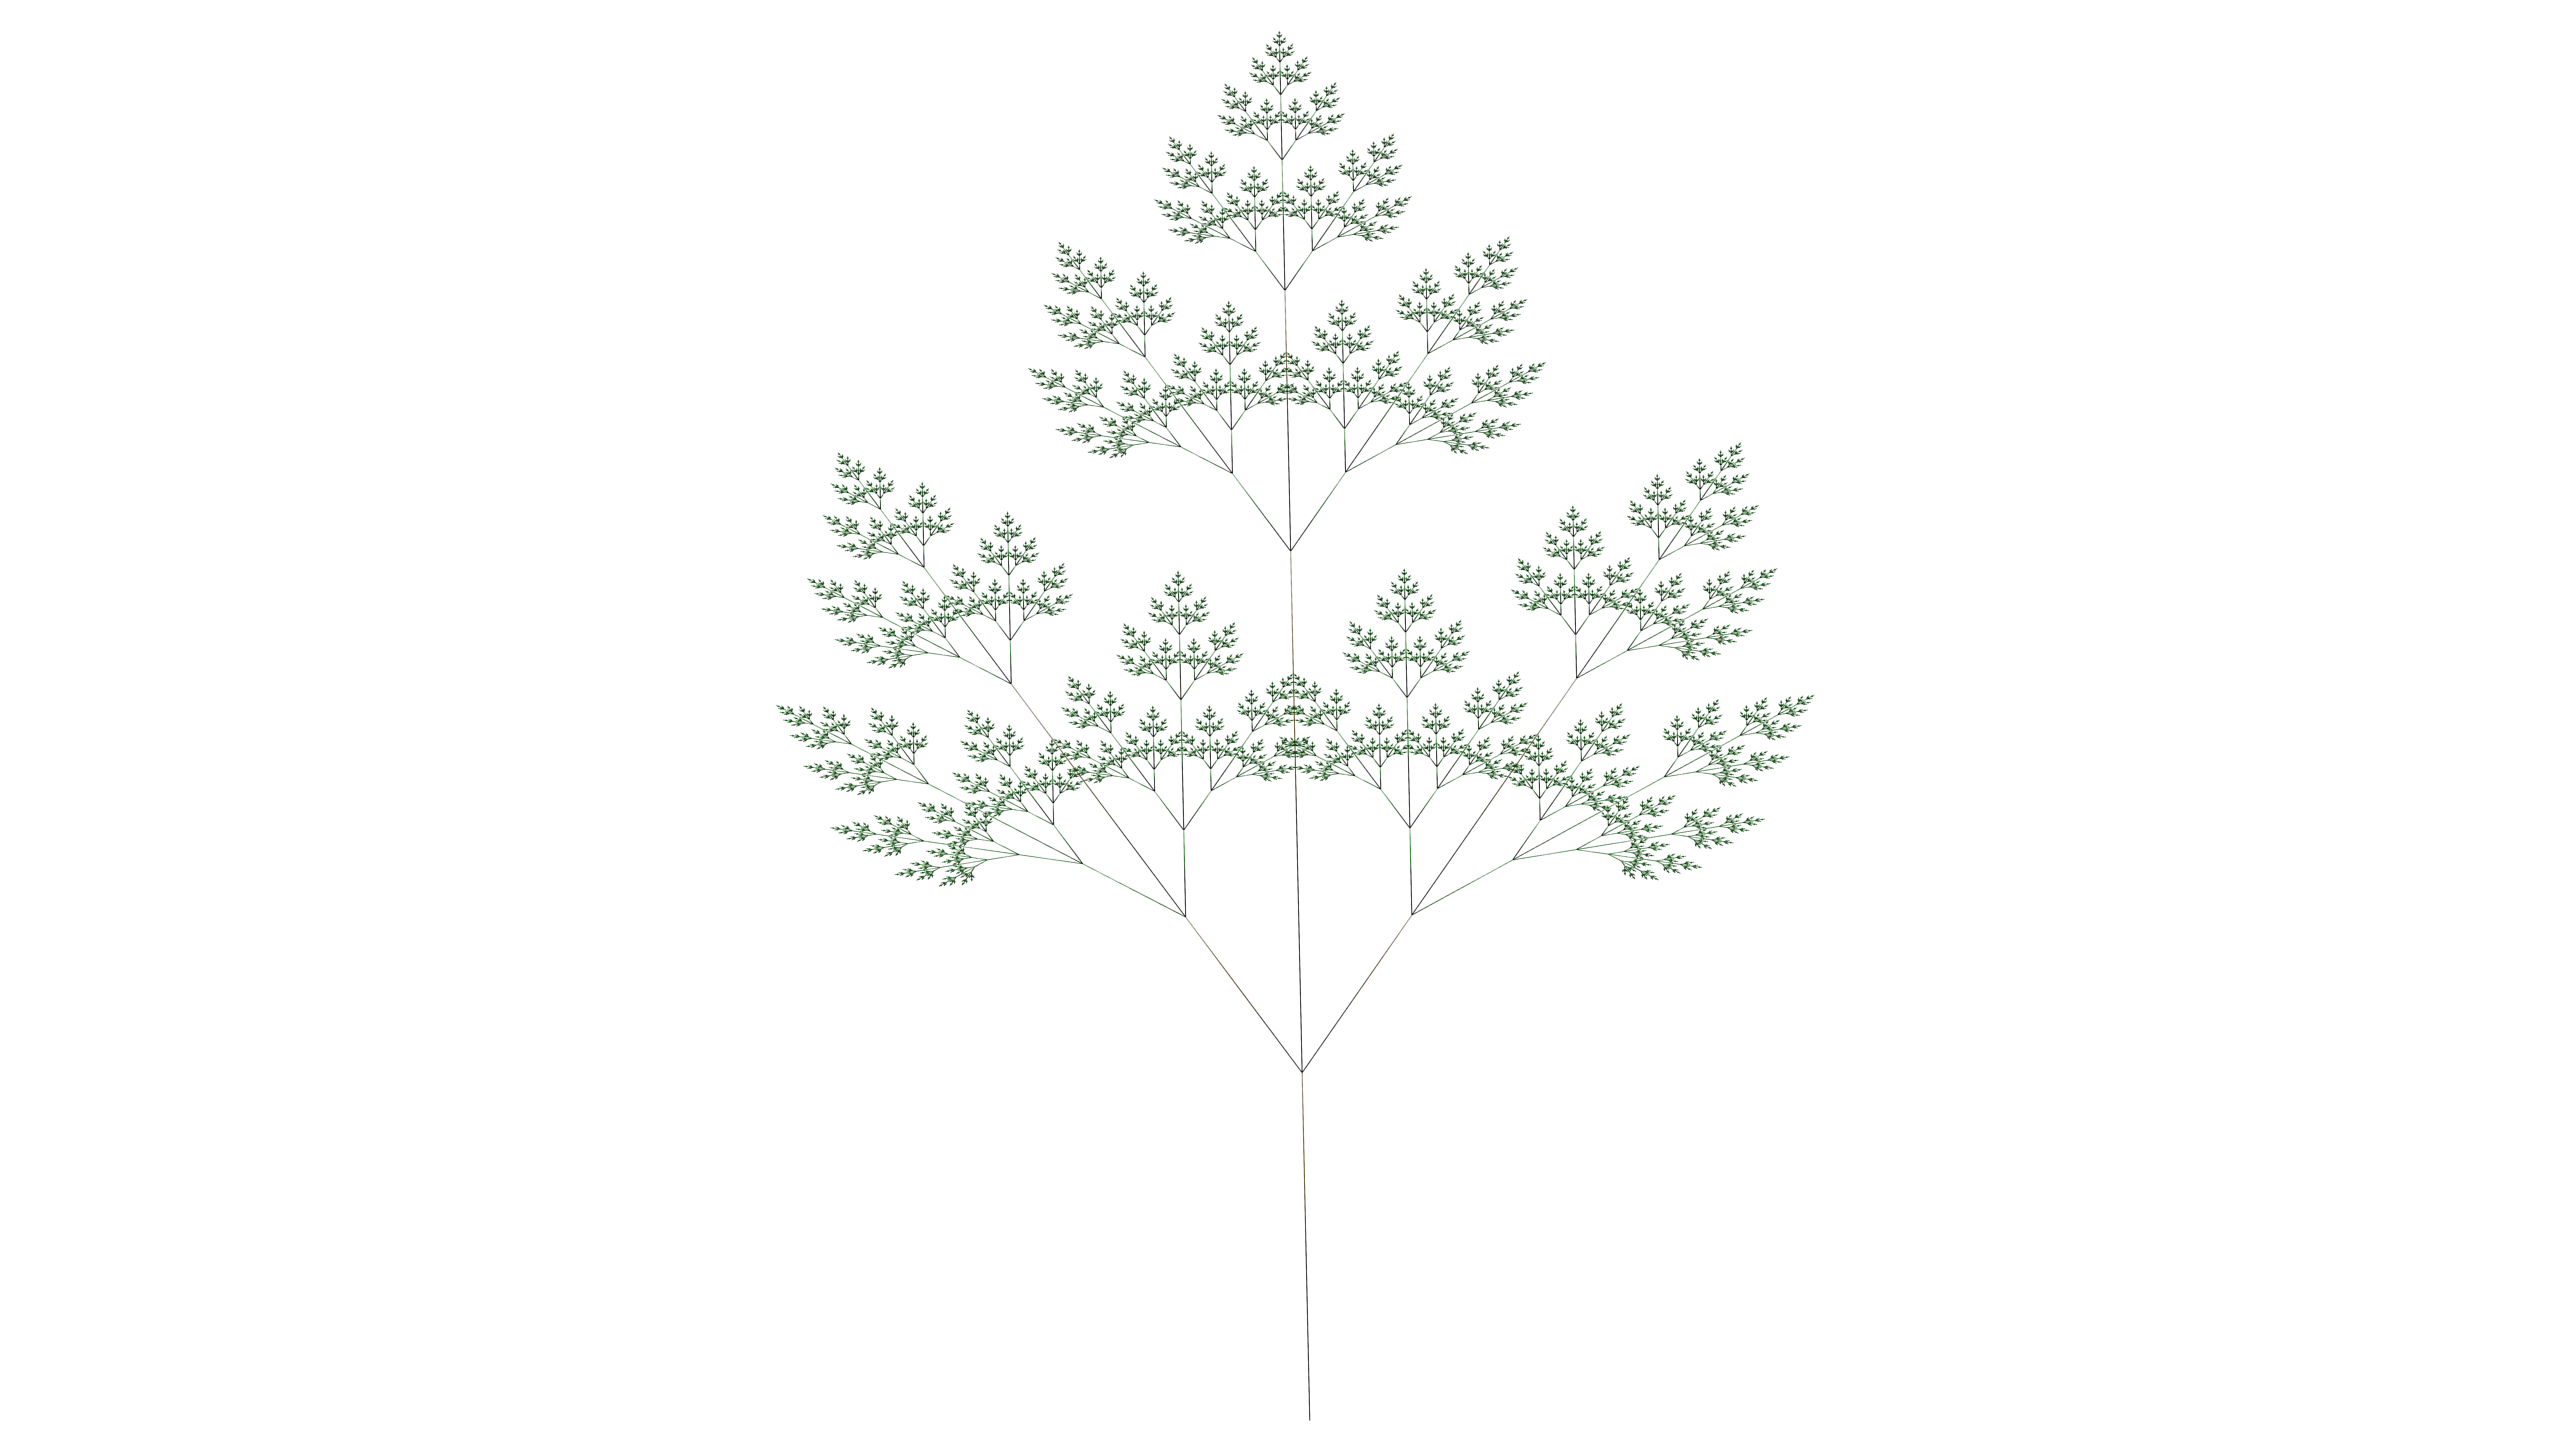
\includegraphics[width=0.90\textwidth]{figures/L-systems/e.png}
    \caption{Problem 2e}\label{fig:prob2e}
\end{figure}

\begin{figure}[H]
    \centering
    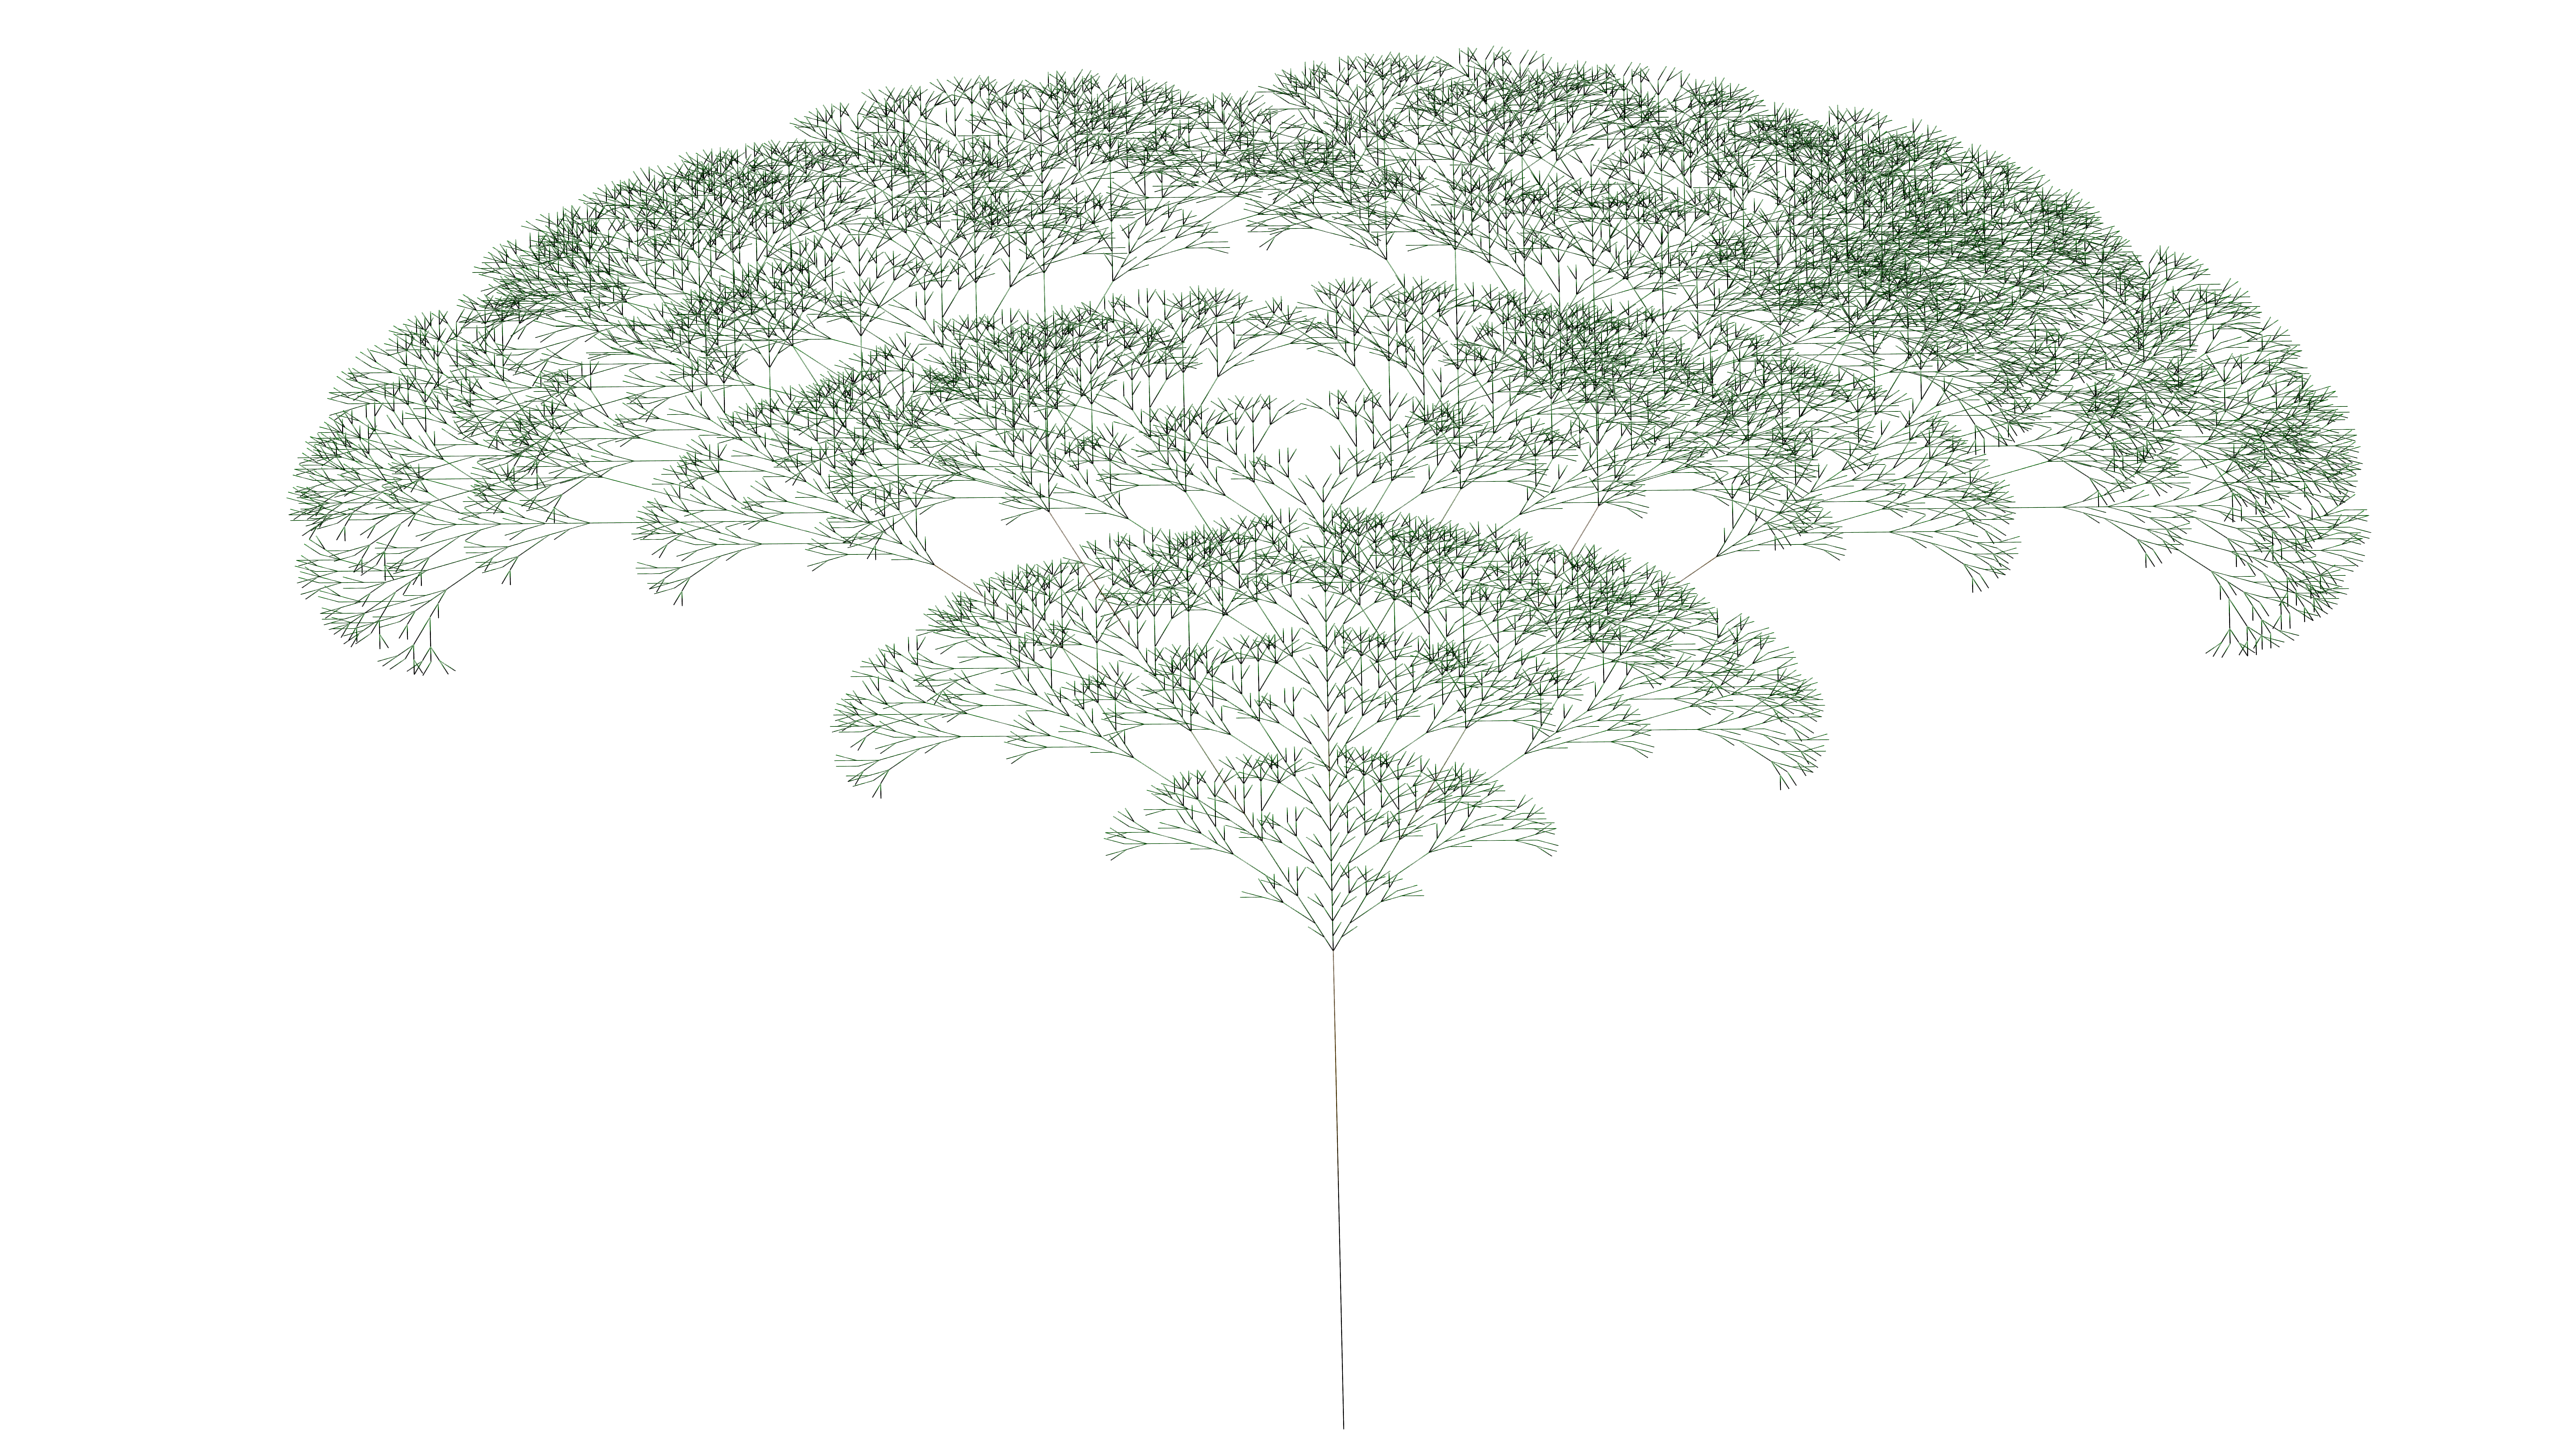
\includegraphics[width=0.90\textwidth]{figures/L-systems/f.png}
    \caption{Problem 2f}\label{fig:prob2f}
\end{figure}

\subsubsection{Expanding the Lindenmayer Systems to 3D}
We attempted to add an extra dimension to each of the items in \autoref{sec:p2-results}.
We also experimented with classical systems such as
Sierpiński triangle, Cantor Set, Dragon, Koch, and variants of our own design.

\begin{figure}[H]
    \centering
    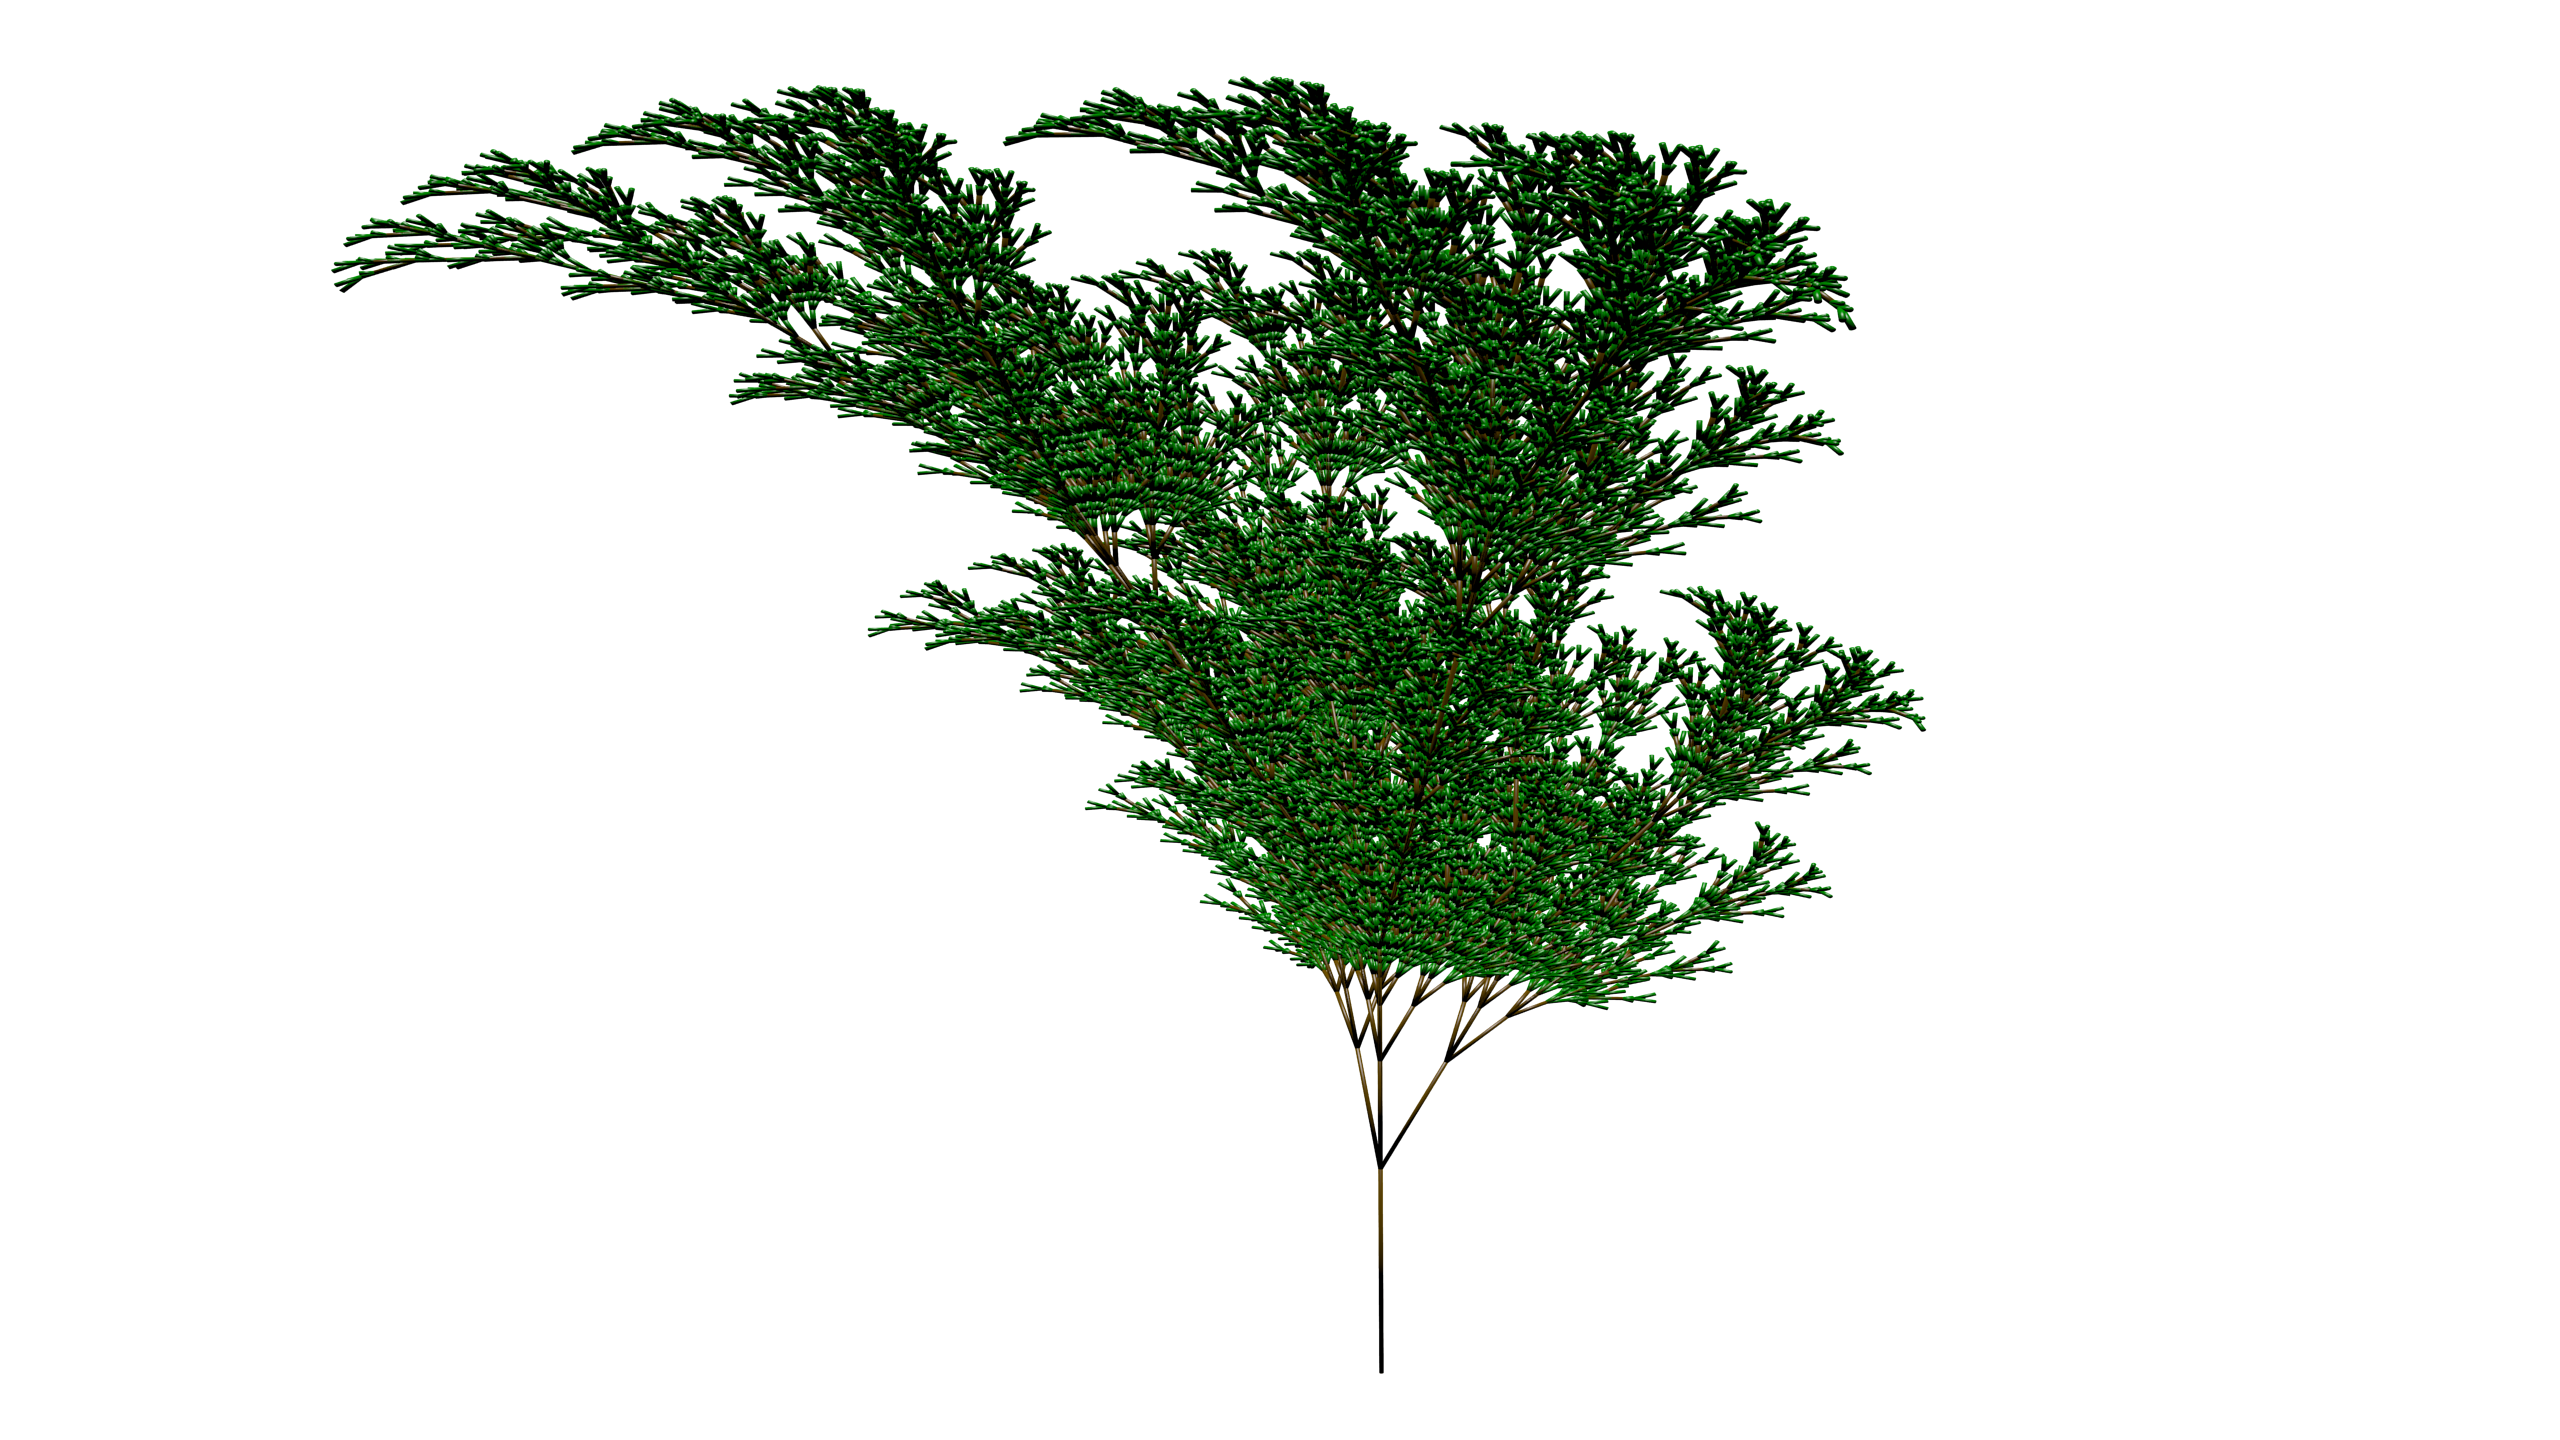
\includegraphics[width=0.90\textwidth]{figures/L-systems/a3d.png}
    \caption{Problem 2a 3D}\label{fig:prob2a_3d}
\end{figure}

\begin{figure}[H]
    \centering
    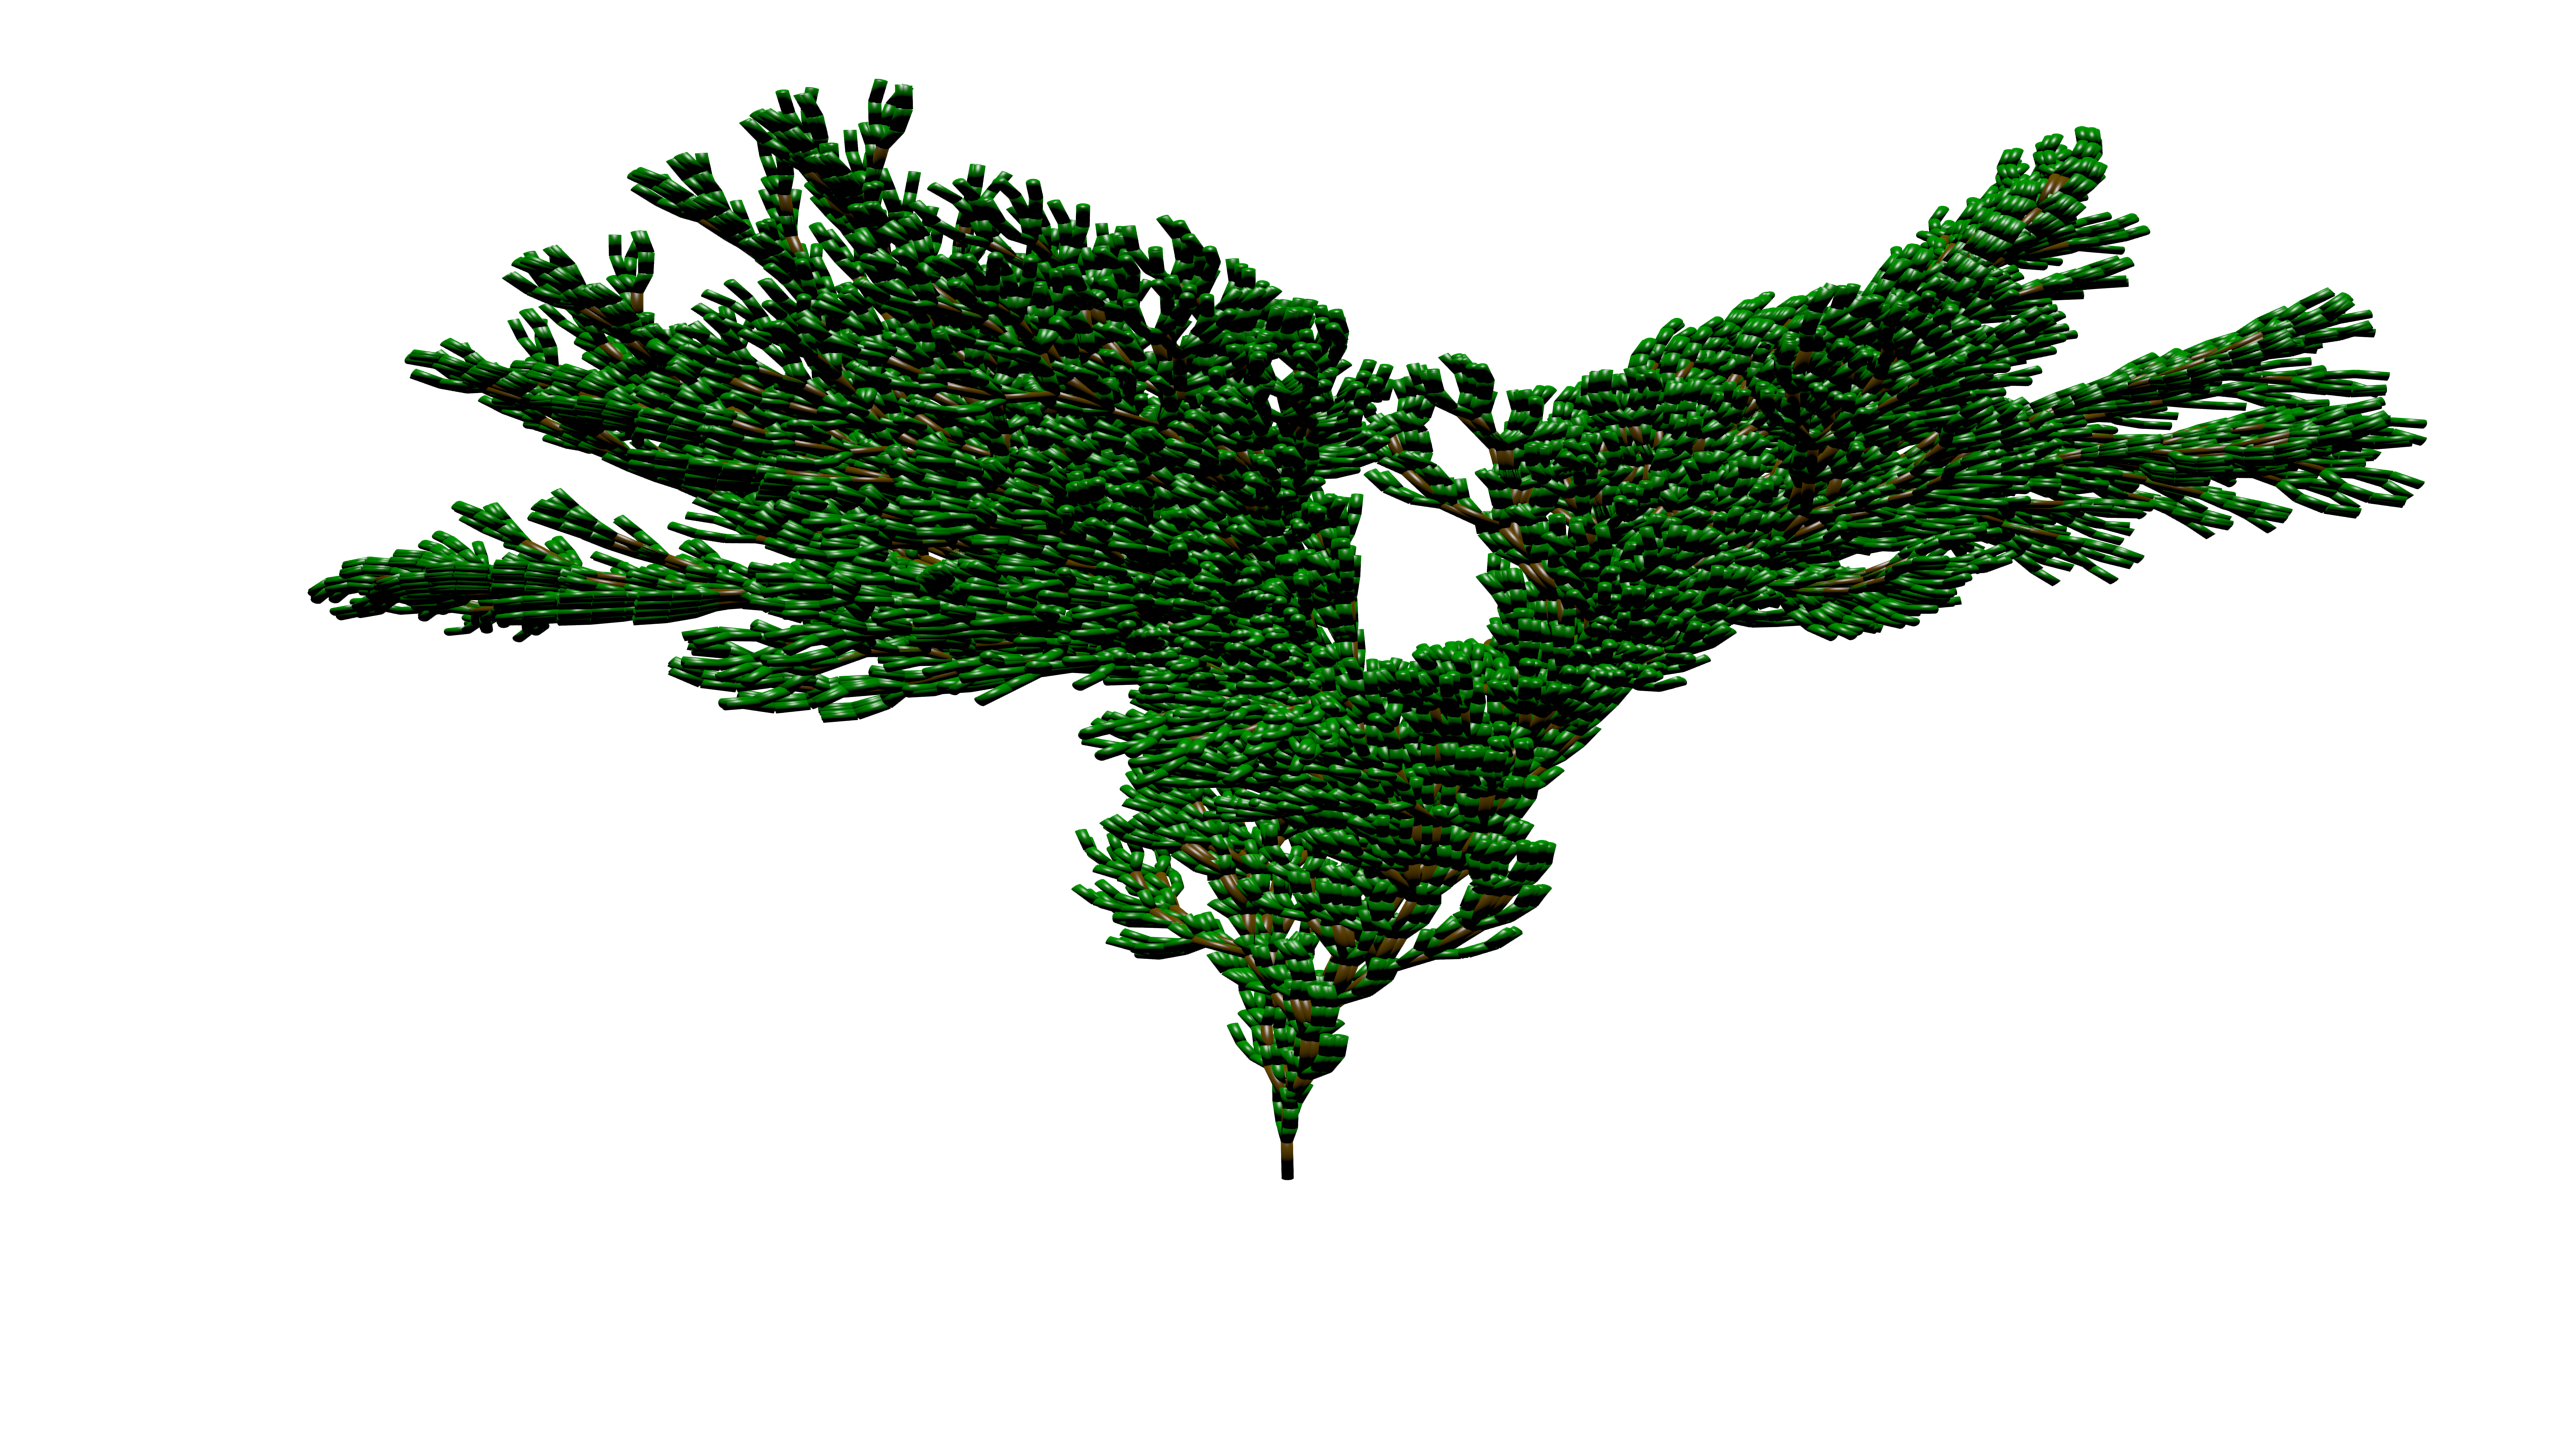
\includegraphics[width=0.90\textwidth]{figures/L-systems/b3d.png}
    \caption{Problem 2b 3D}\label{fig:prob2b_3d}
\end{figure}

\begin{figure}[H]
    \centering
    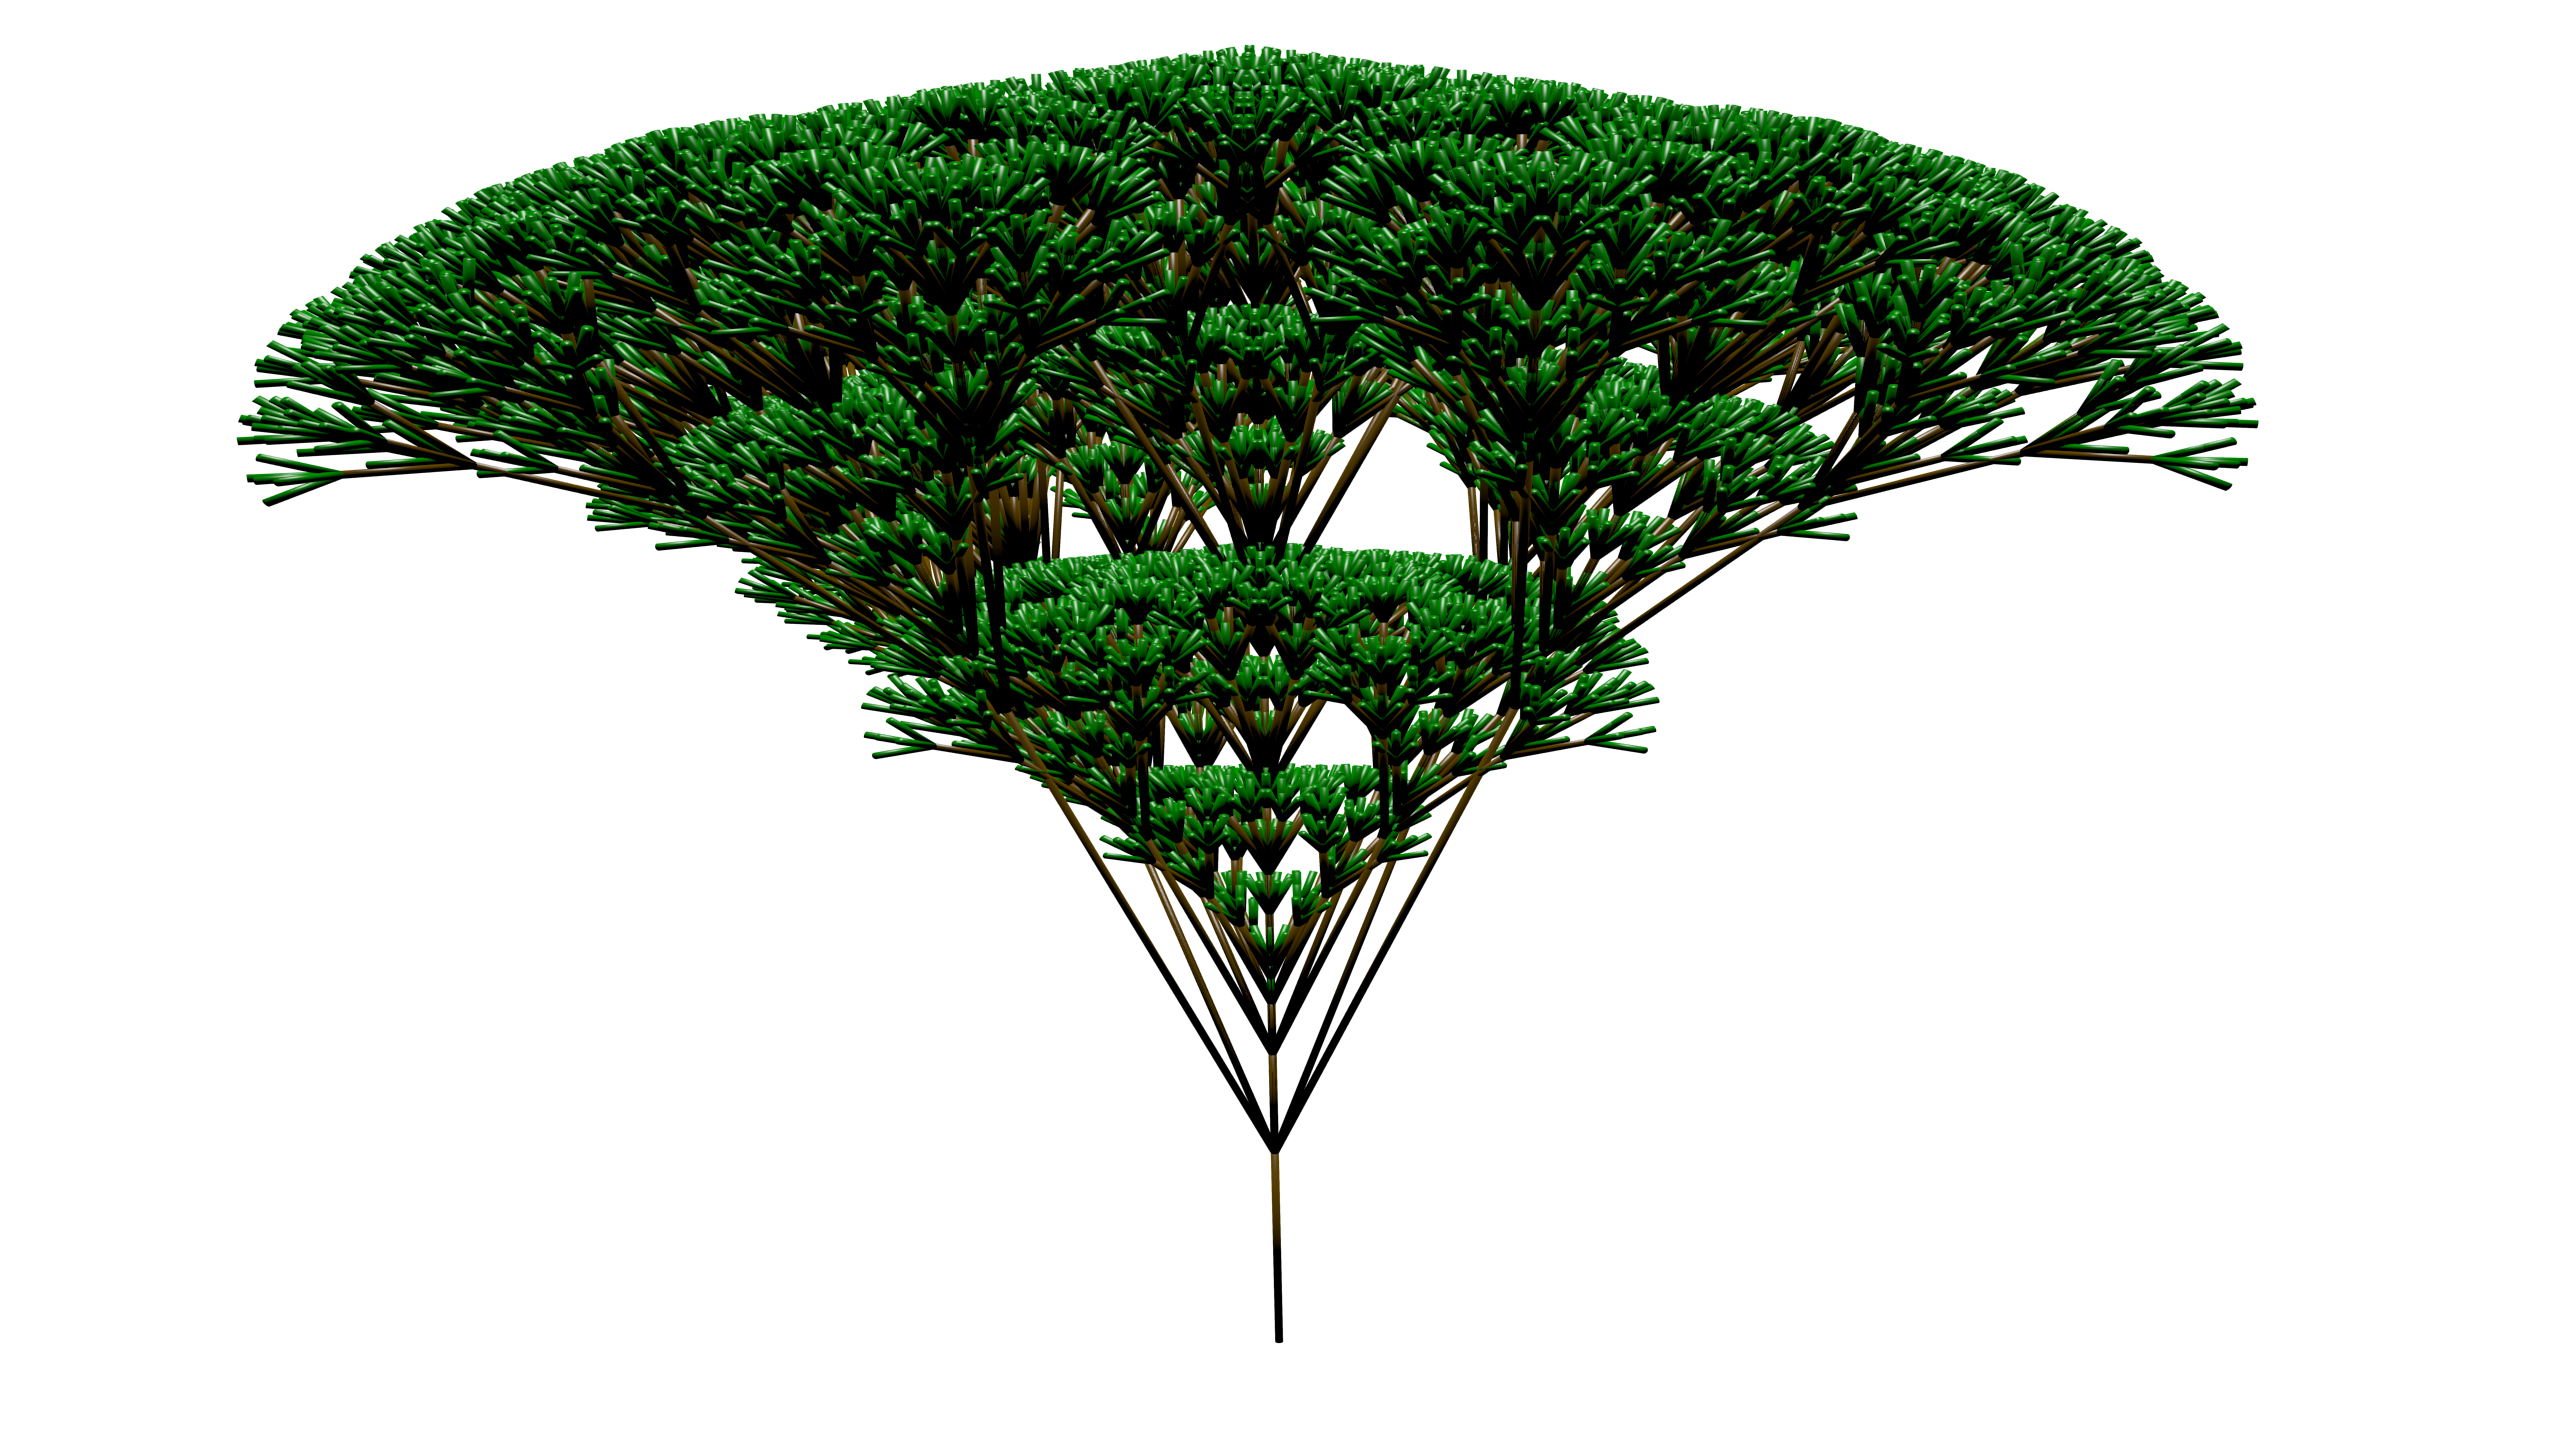
\includegraphics[width=0.90\textwidth]{figures/L-systems/c3d.png}
    \caption{Problem 2c 3D}\label{fig:prob2c_3d}
\end{figure}

\begin{figure}[H]
    \centering
    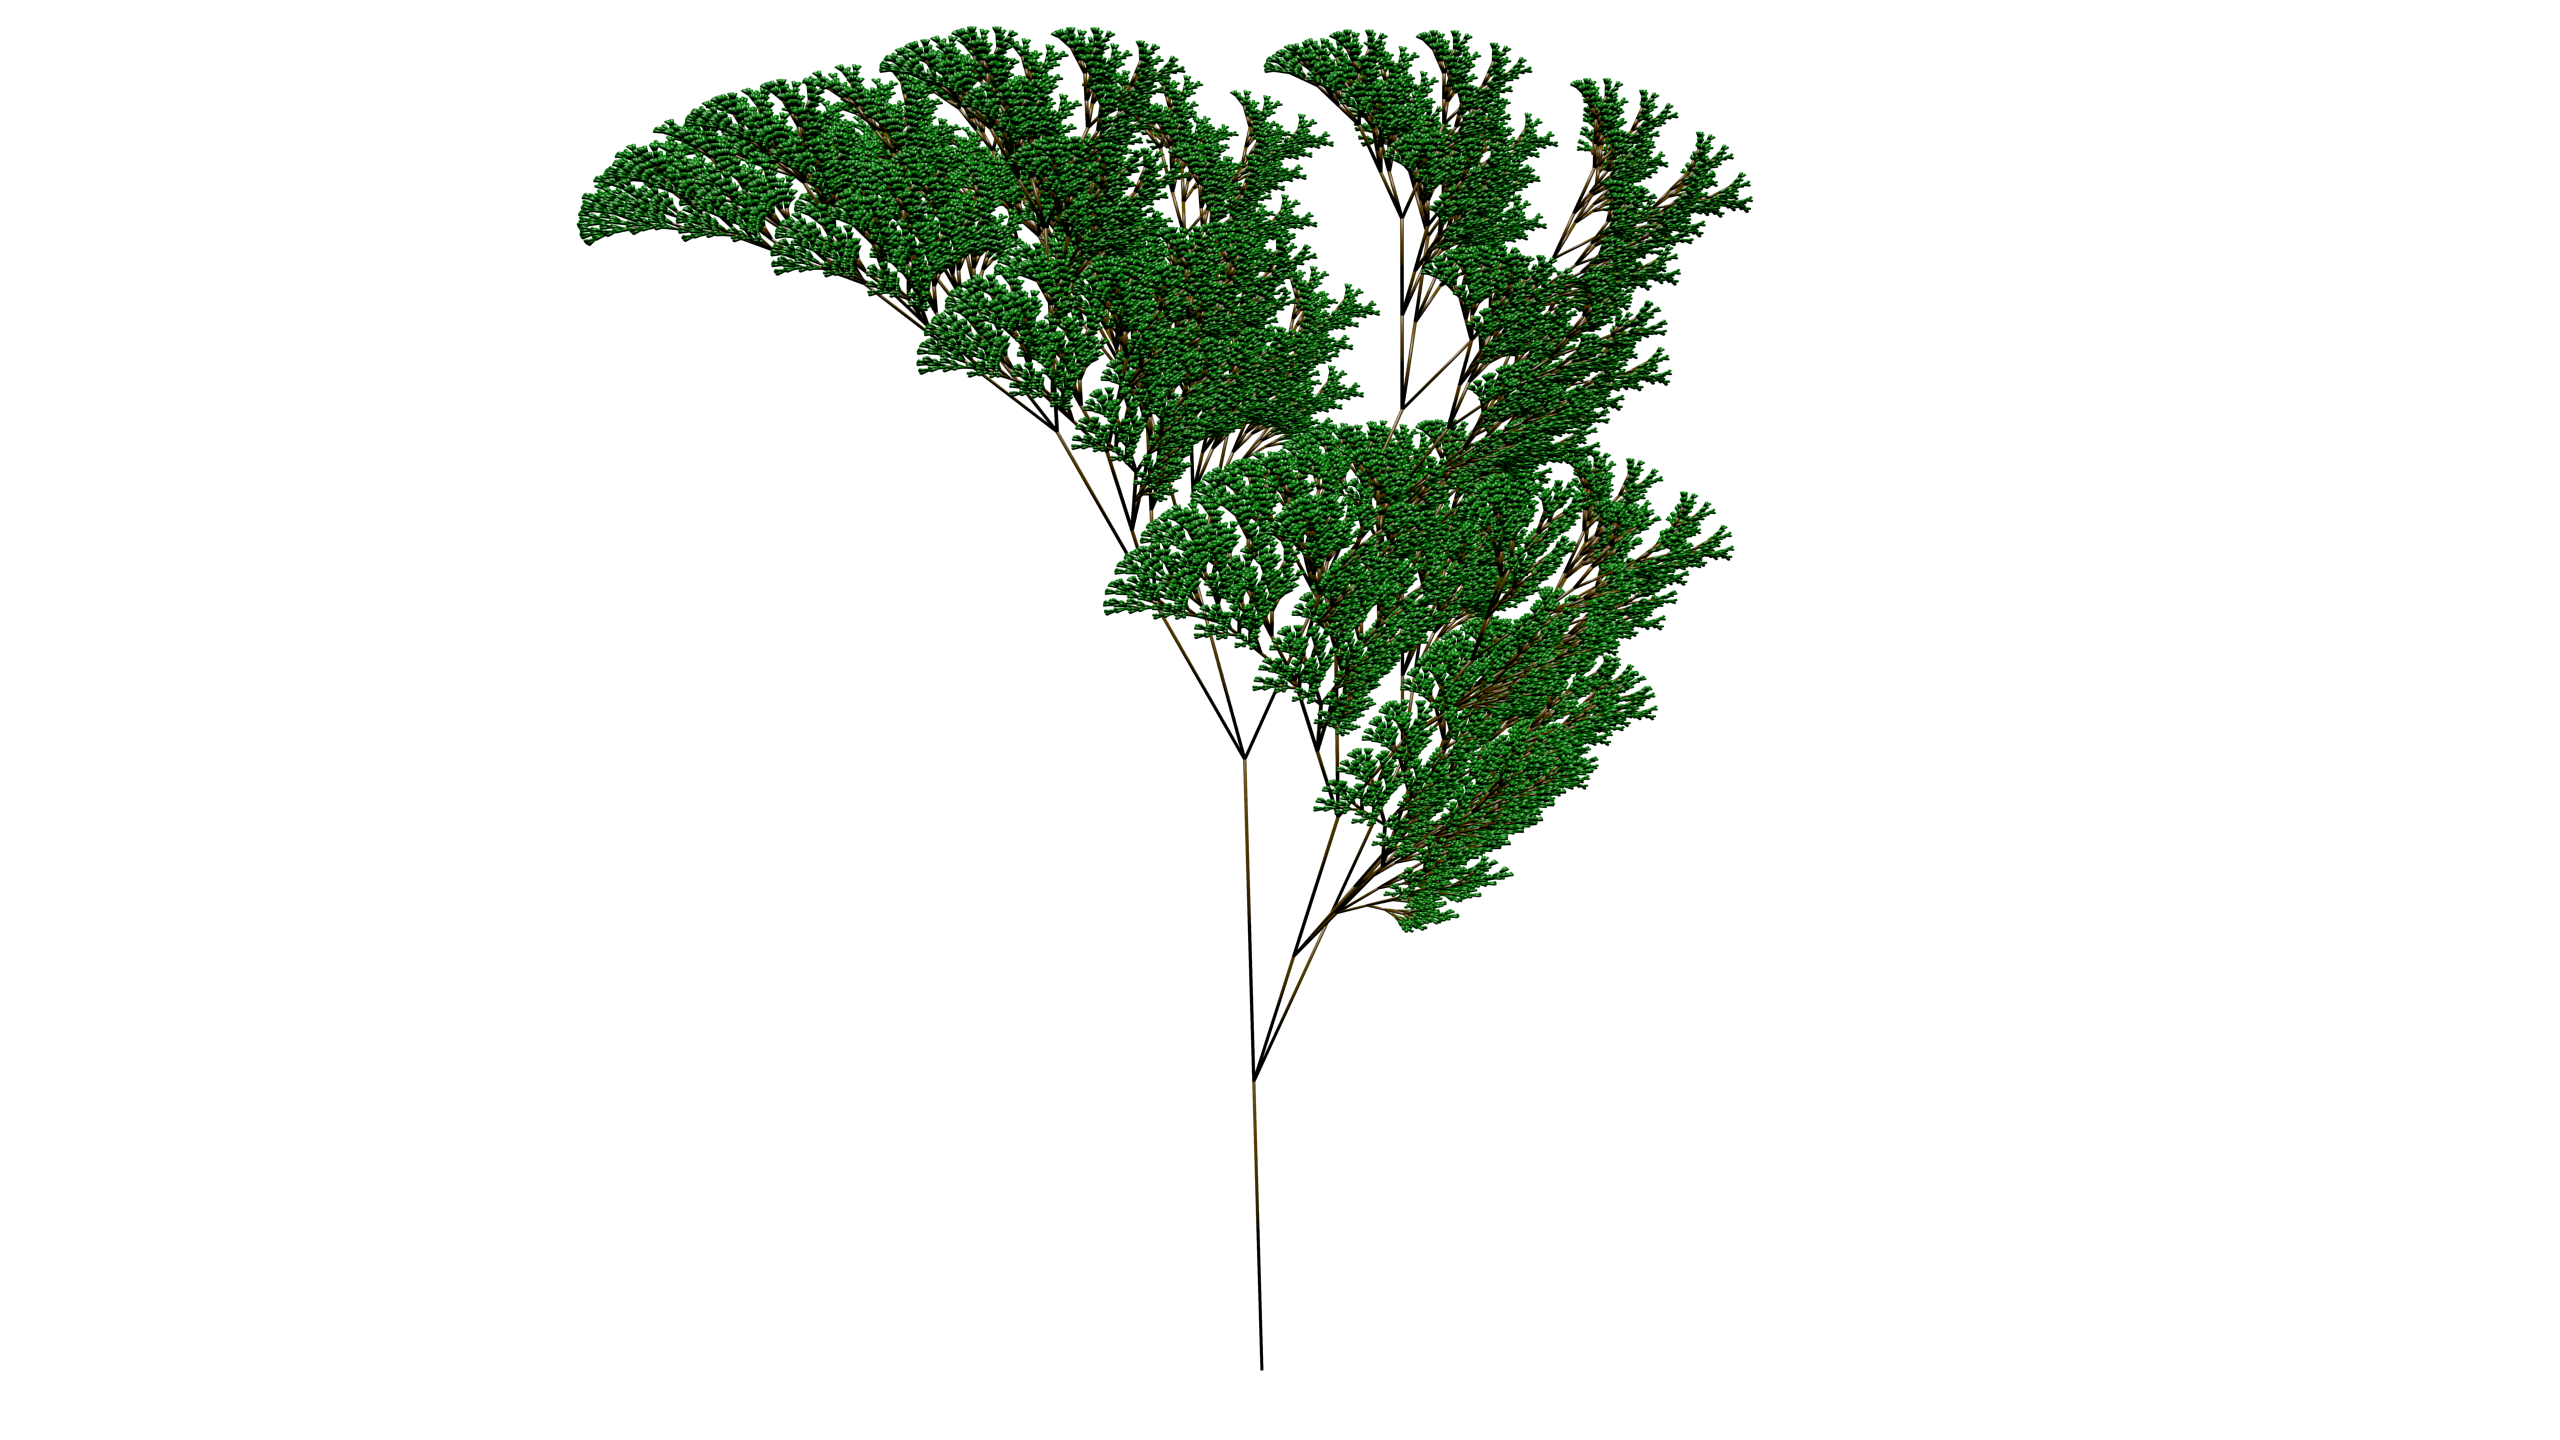
\includegraphics[width=0.90\textwidth]{figures/L-systems/d3d.png}
    \caption{Problem 2d 3D}\label{fig:prob2d_3d}
\end{figure}

\begin{figure}[H]
    \centering
    \noindent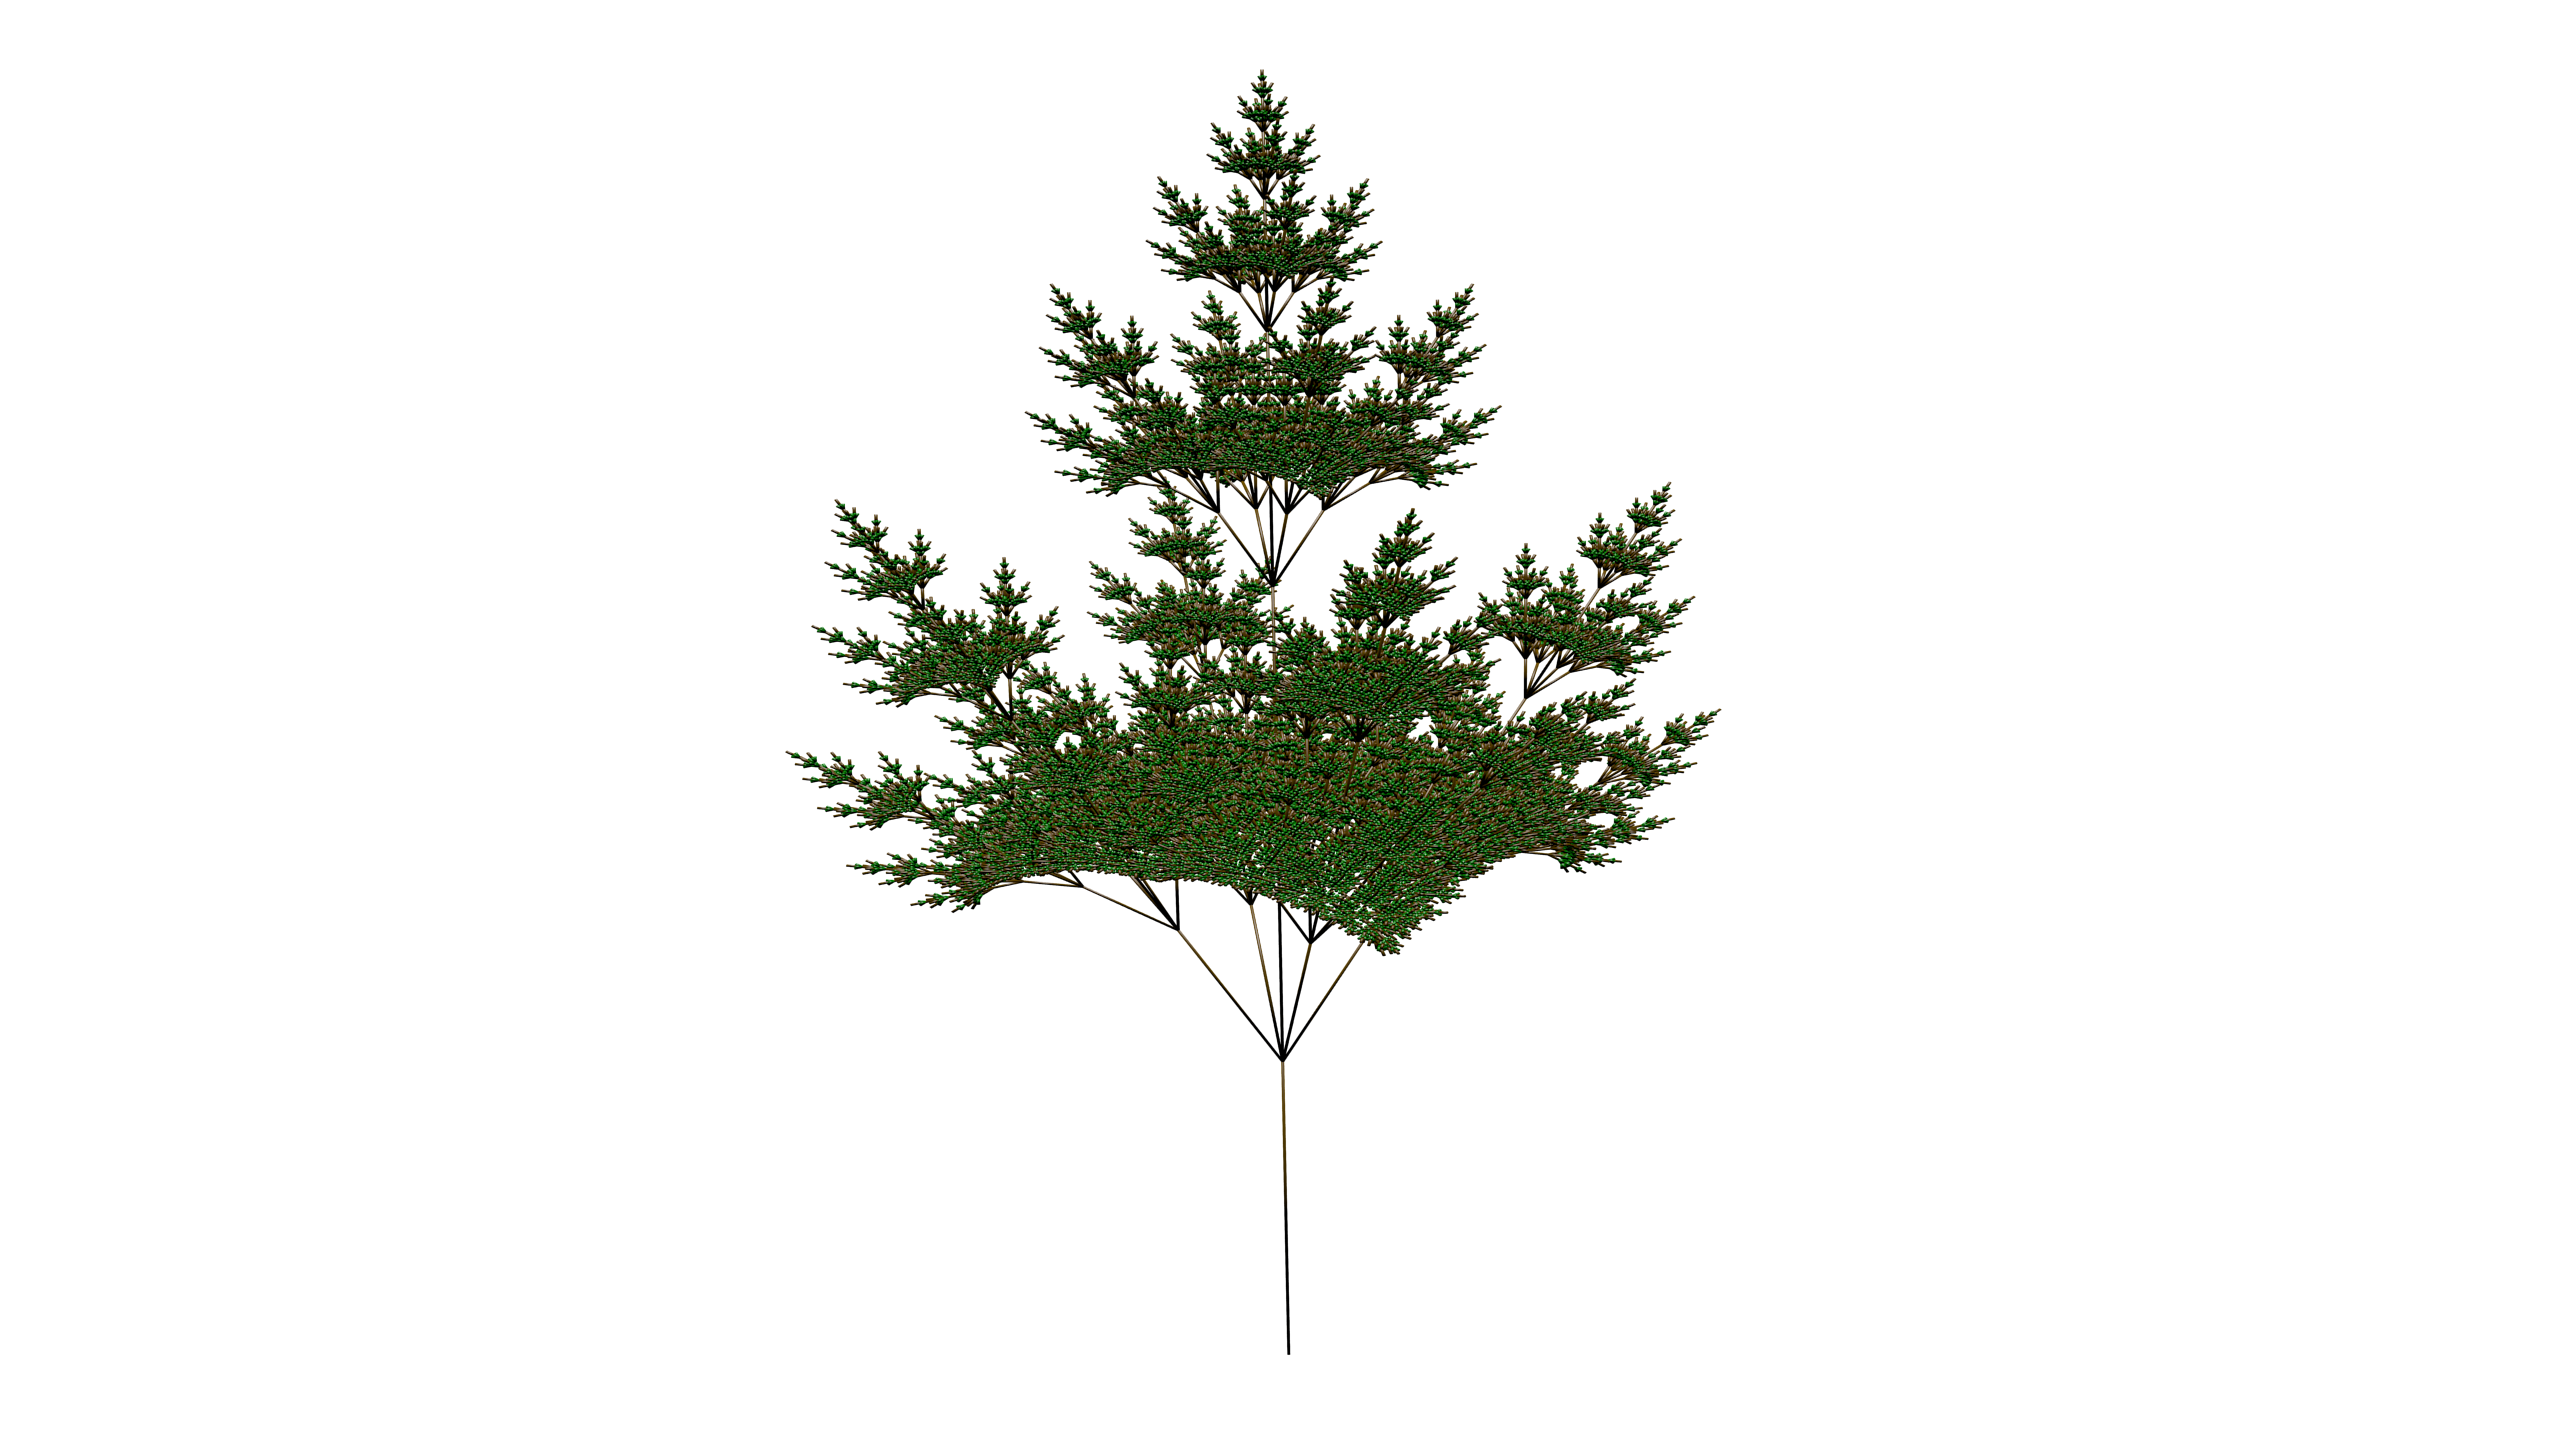
\includegraphics[width=0.90\textwidth]{figures/L-systems/e3d.png}
    \caption{Problem 2e 3D}\label{fig:prob2e_3d}
\end{figure}

\begin{figure}[H]
    \centering
    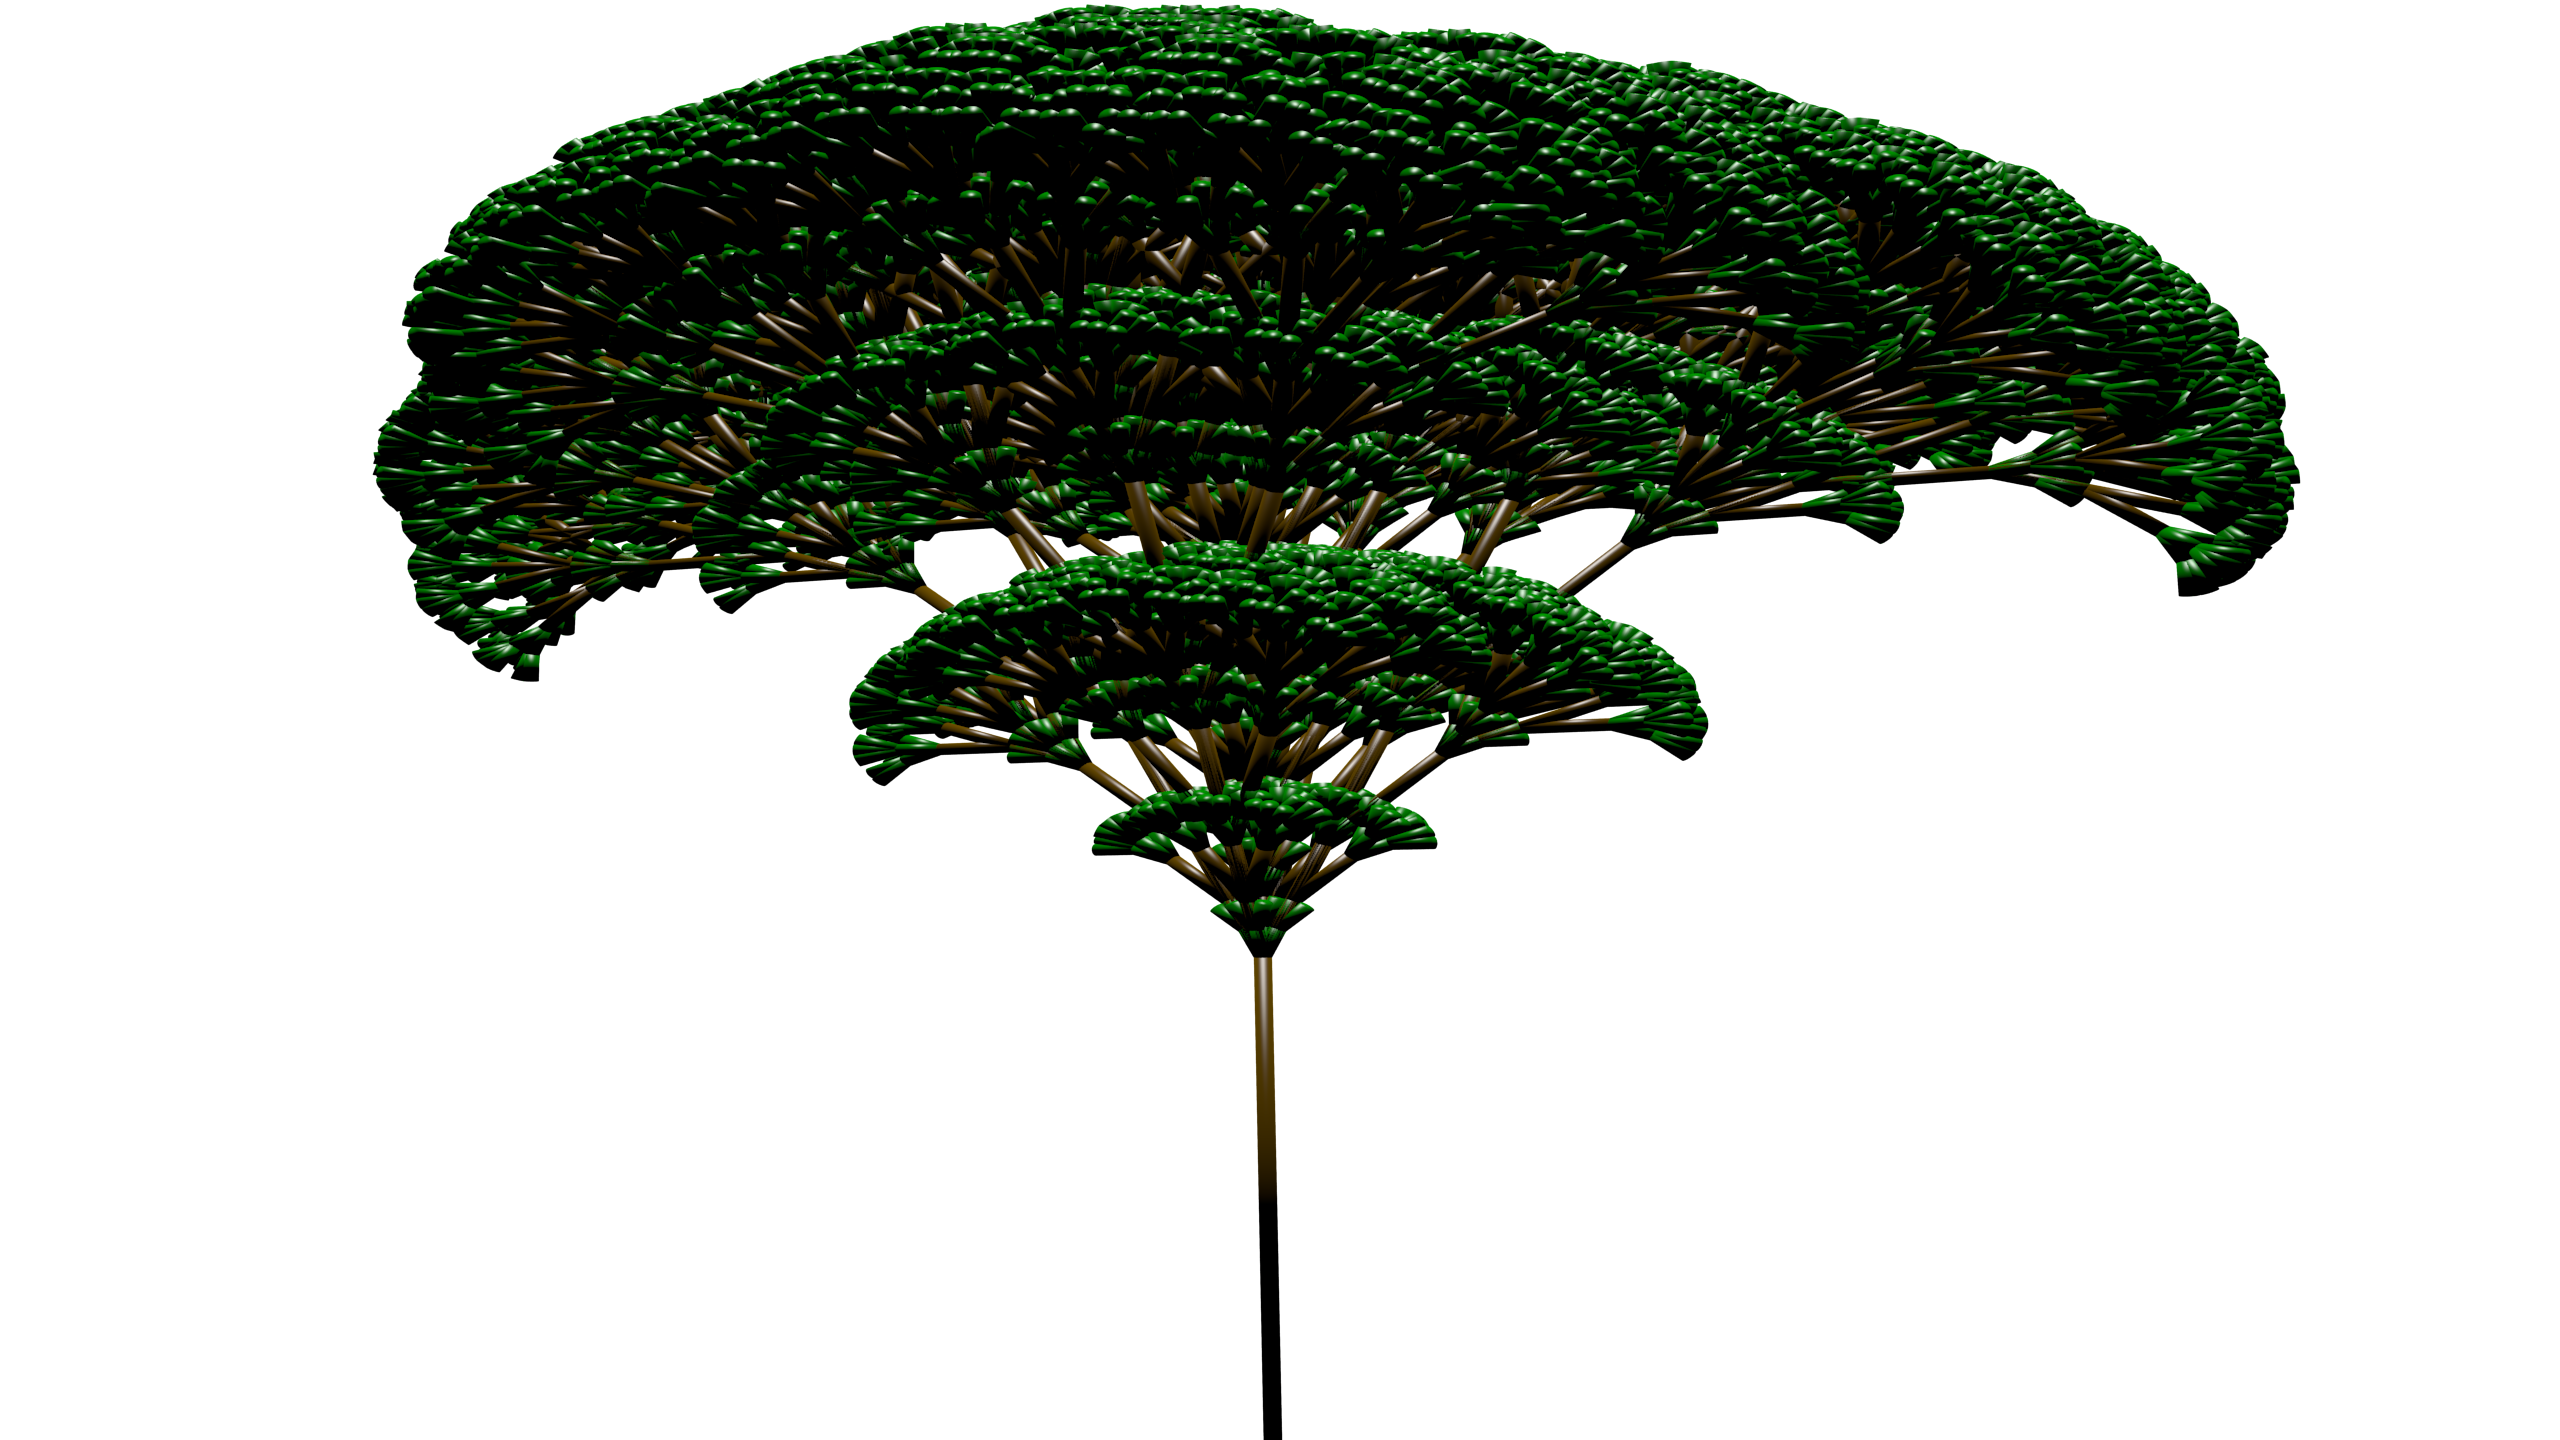
\includegraphics[width=0.90\textwidth]{figures/L-systems/f3d.png}
    \caption{Problem 2f 3D}\label{fig:prob2f_3d}
\end{figure}

\begin{figure}[H]
    \centering
    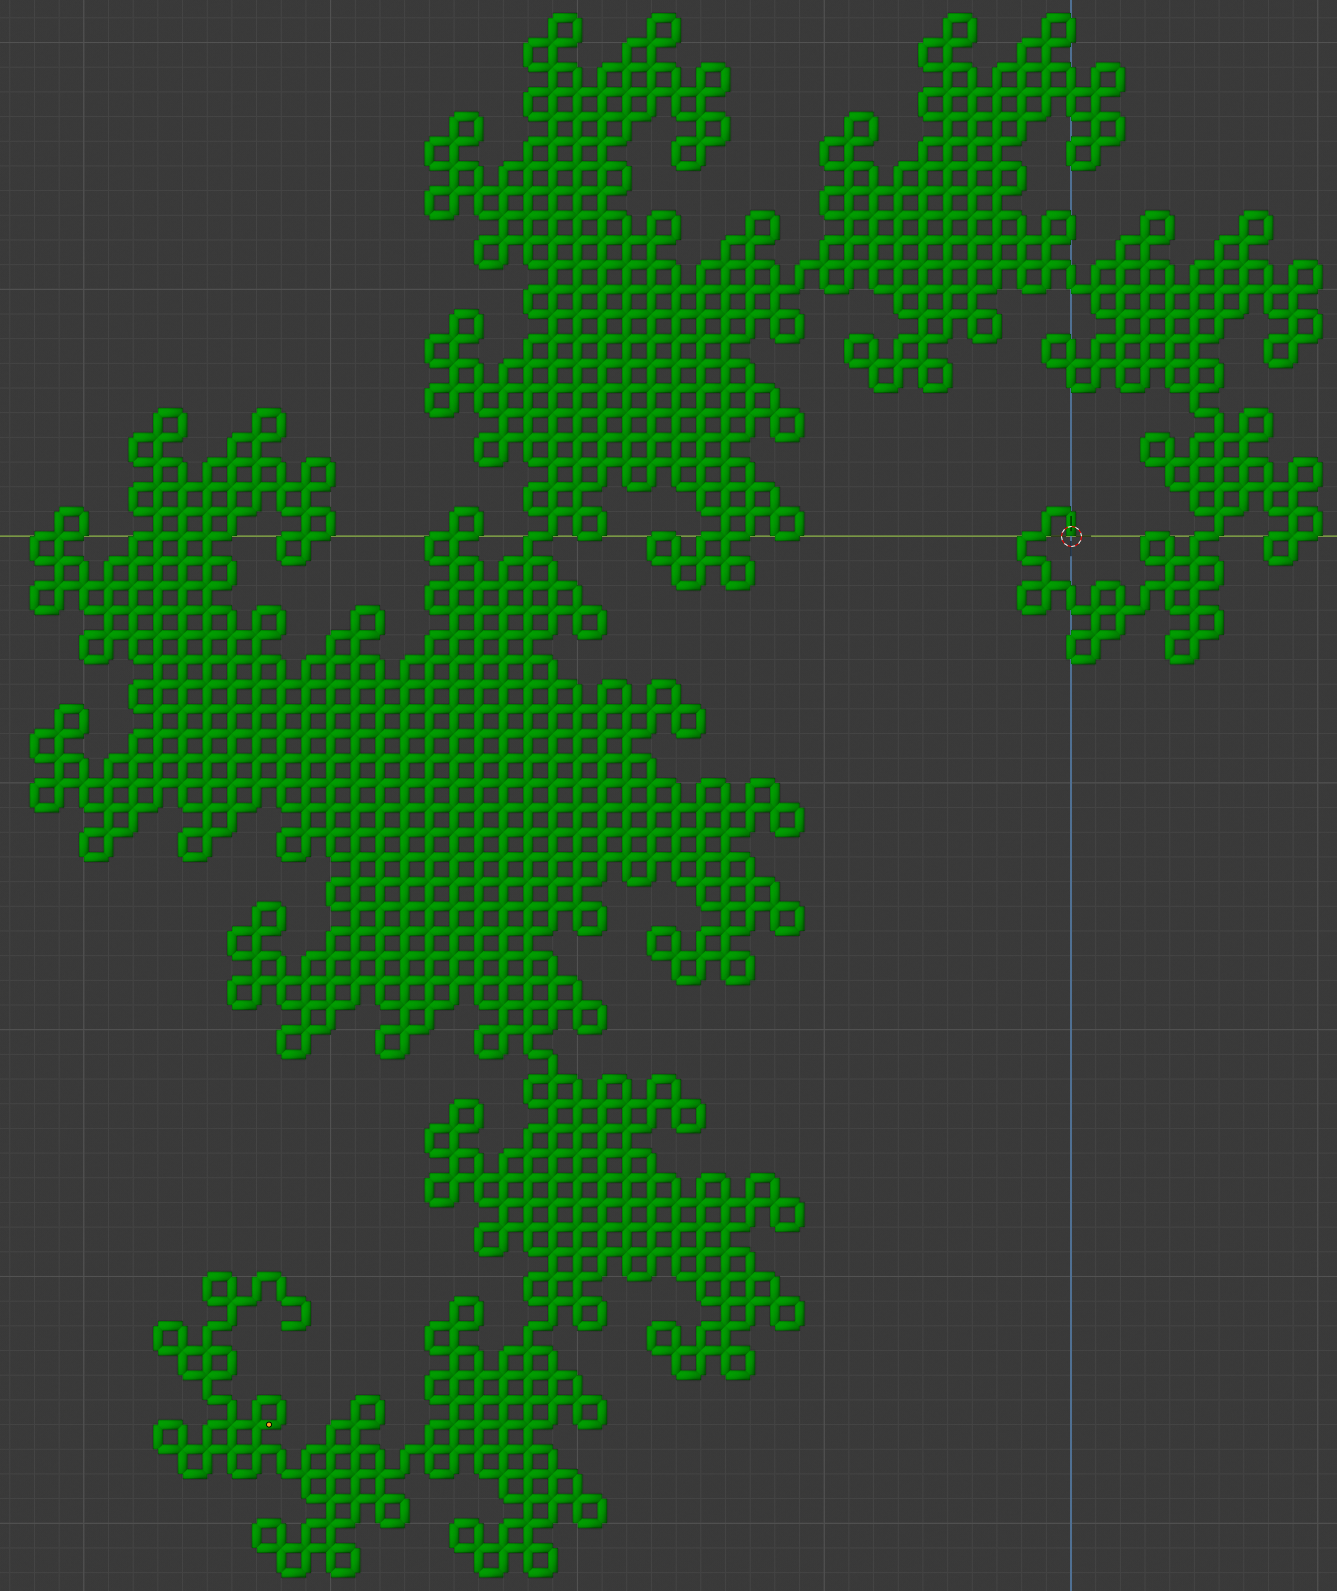
\includegraphics[width=0.7\textwidth]{figures/L-systems/dragon.png}
    \caption{The dragon curve}
\end{figure}

\begin{figure}[H]
    \centering
    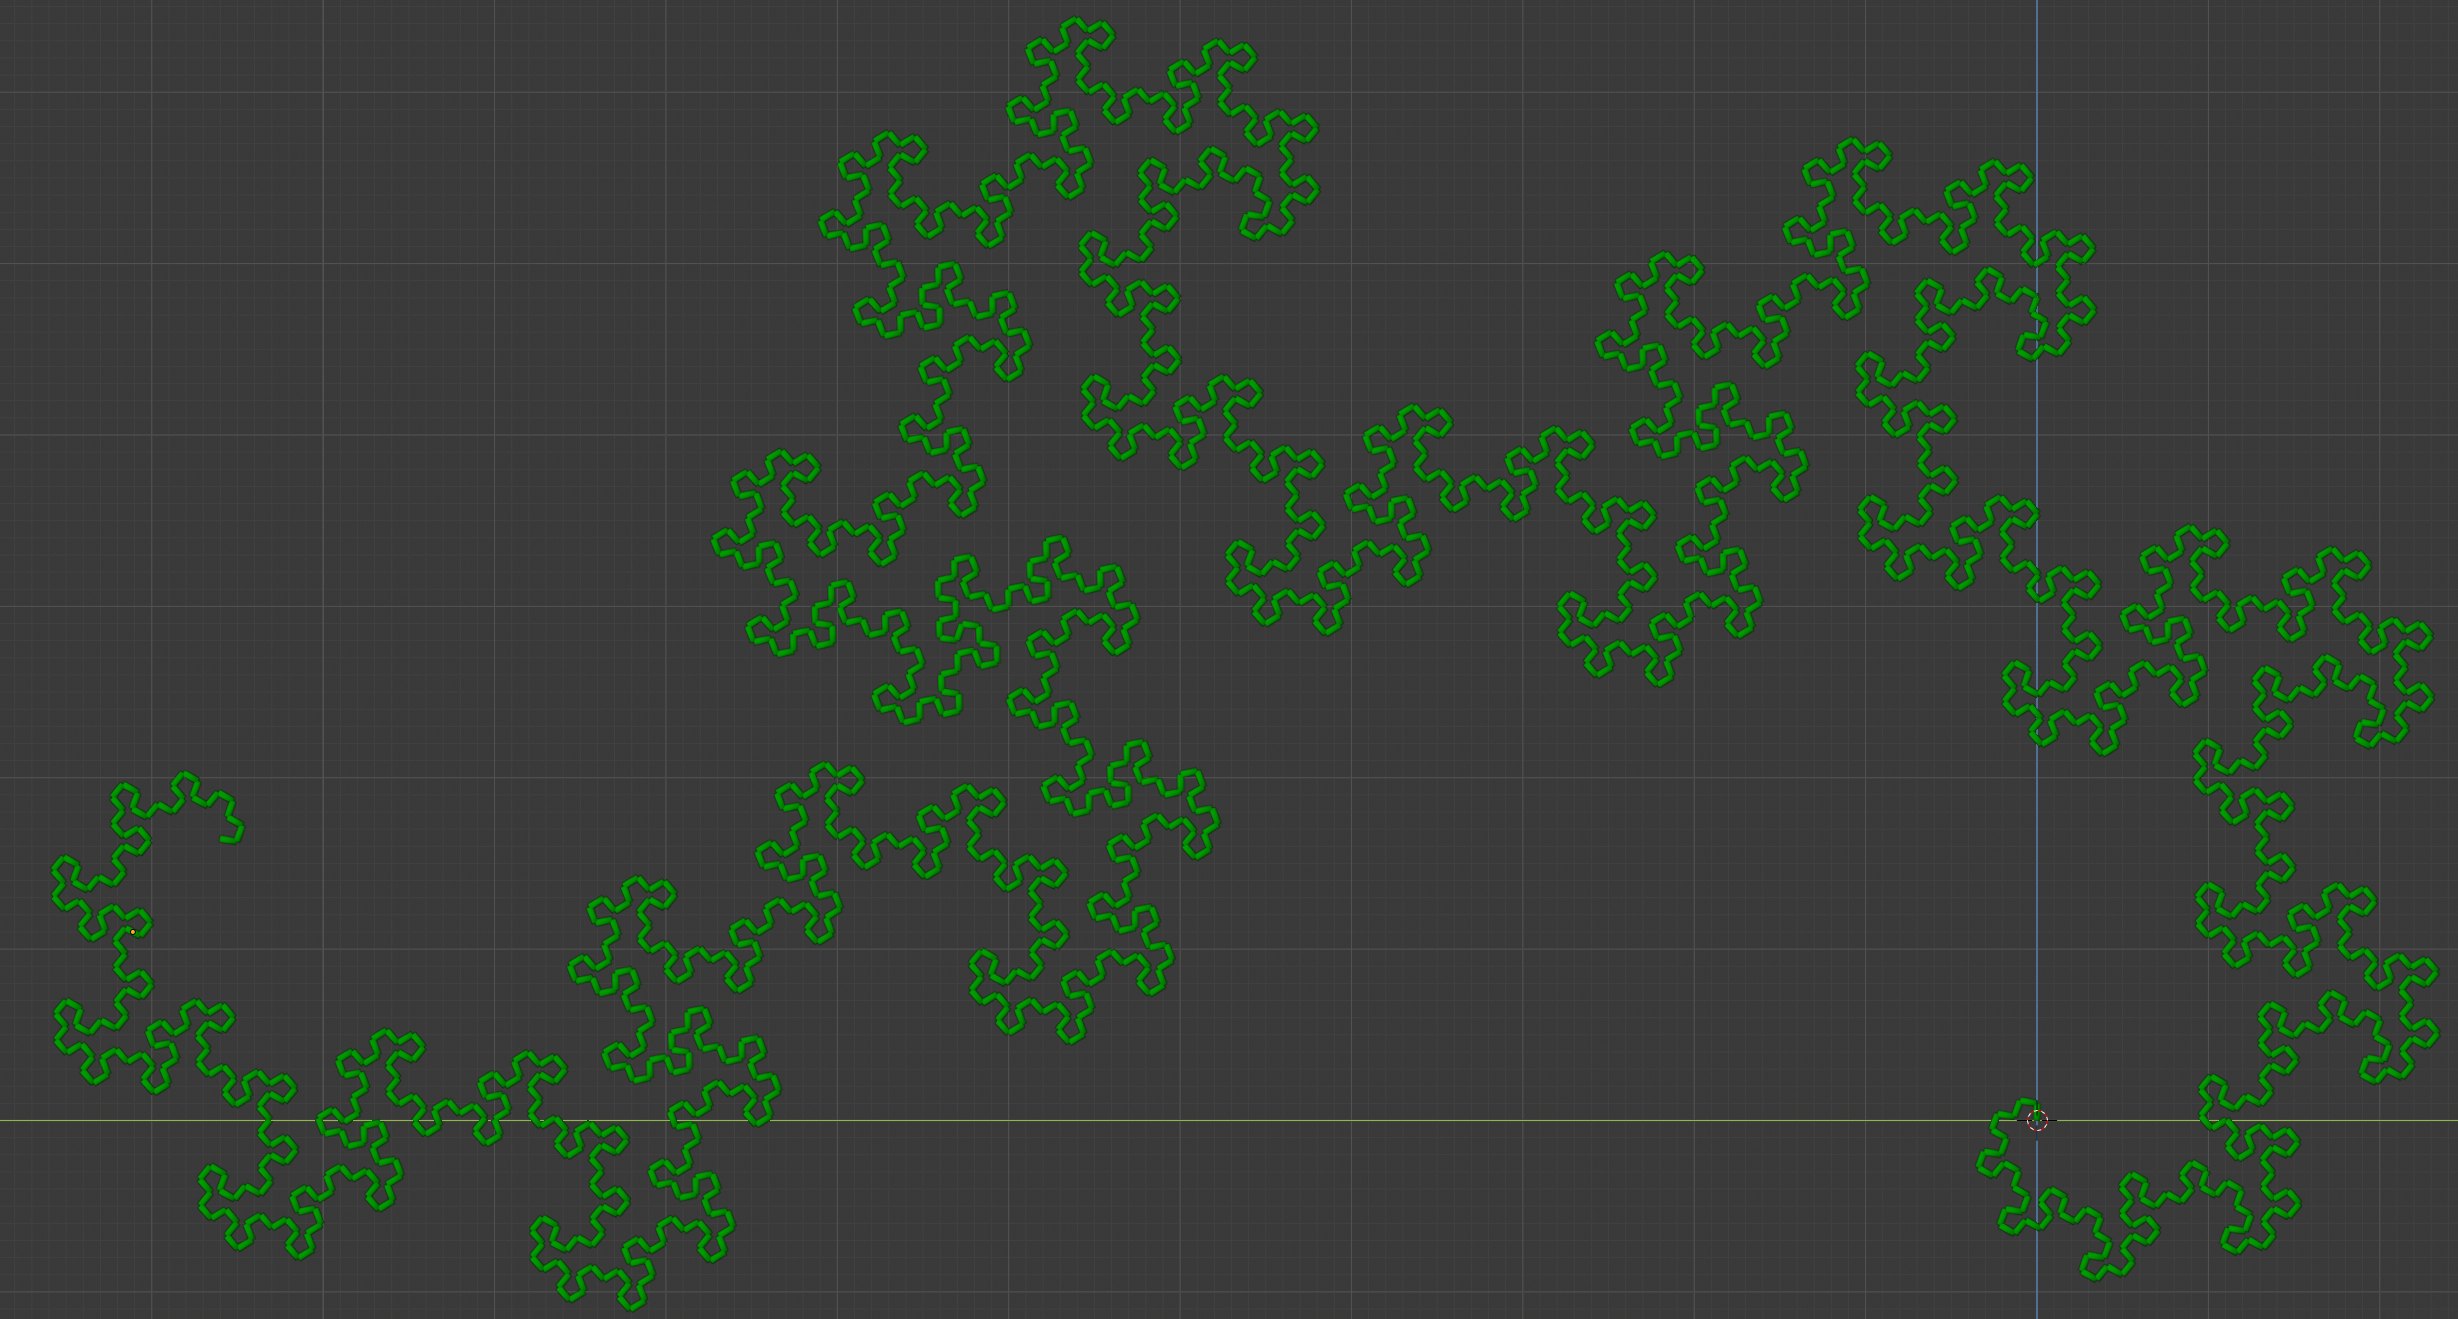
\includegraphics[width=0.7\textwidth]{figures/L-systems/dragon-1_4rad.png}
    \caption{The dragon curve with an angle of 1.4 radians}
\end{figure}

\begin{figure}[H]
    \centering
    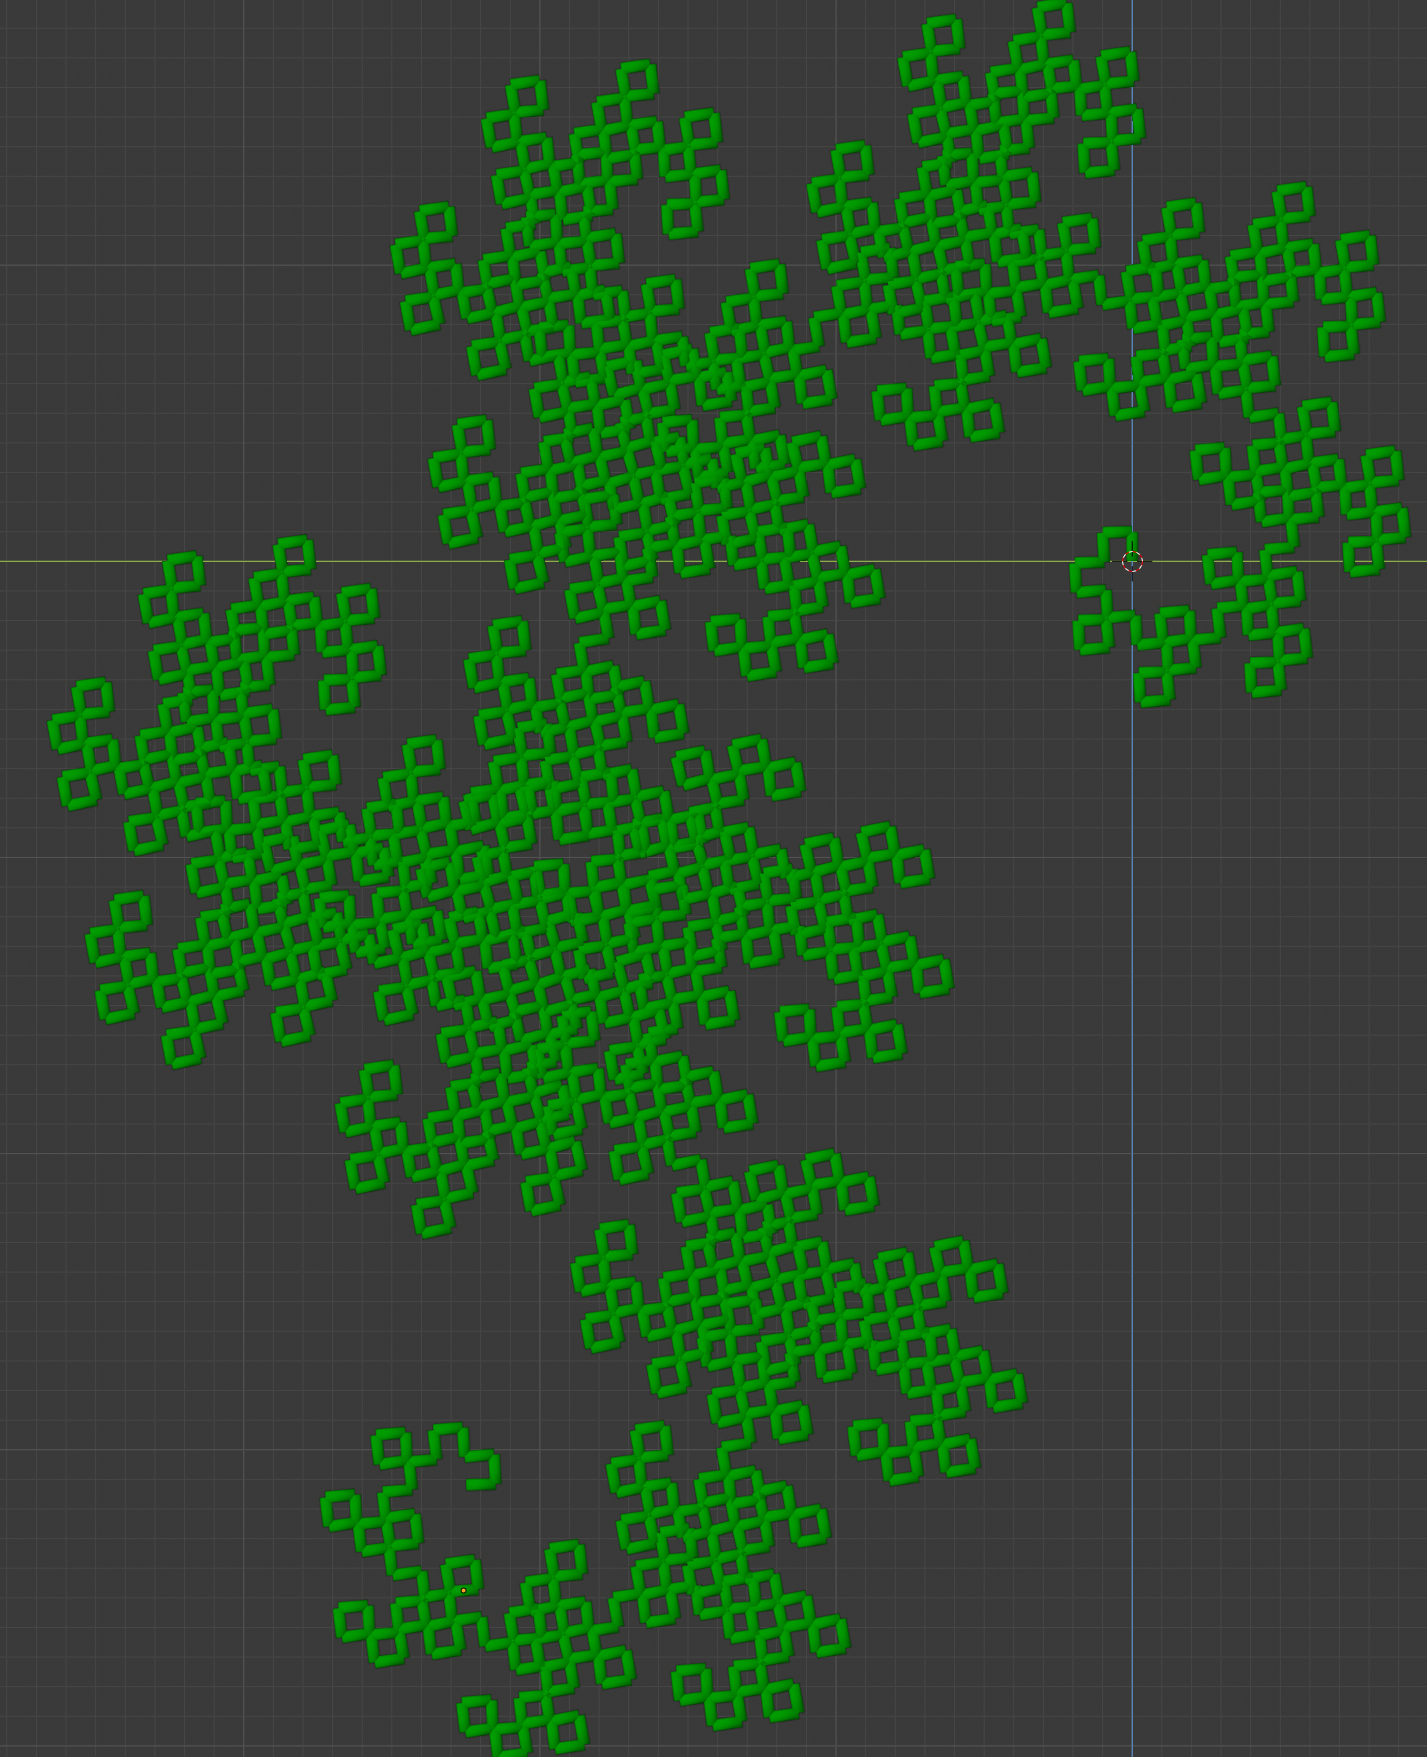
\includegraphics[width=0.7\textwidth]{figures/L-systems/dragon-1_6rad.png}
    \caption{The dragon curve with an angle of 1.6 radians}
\end{figure}

\begin{figure}[H]
    \centering
    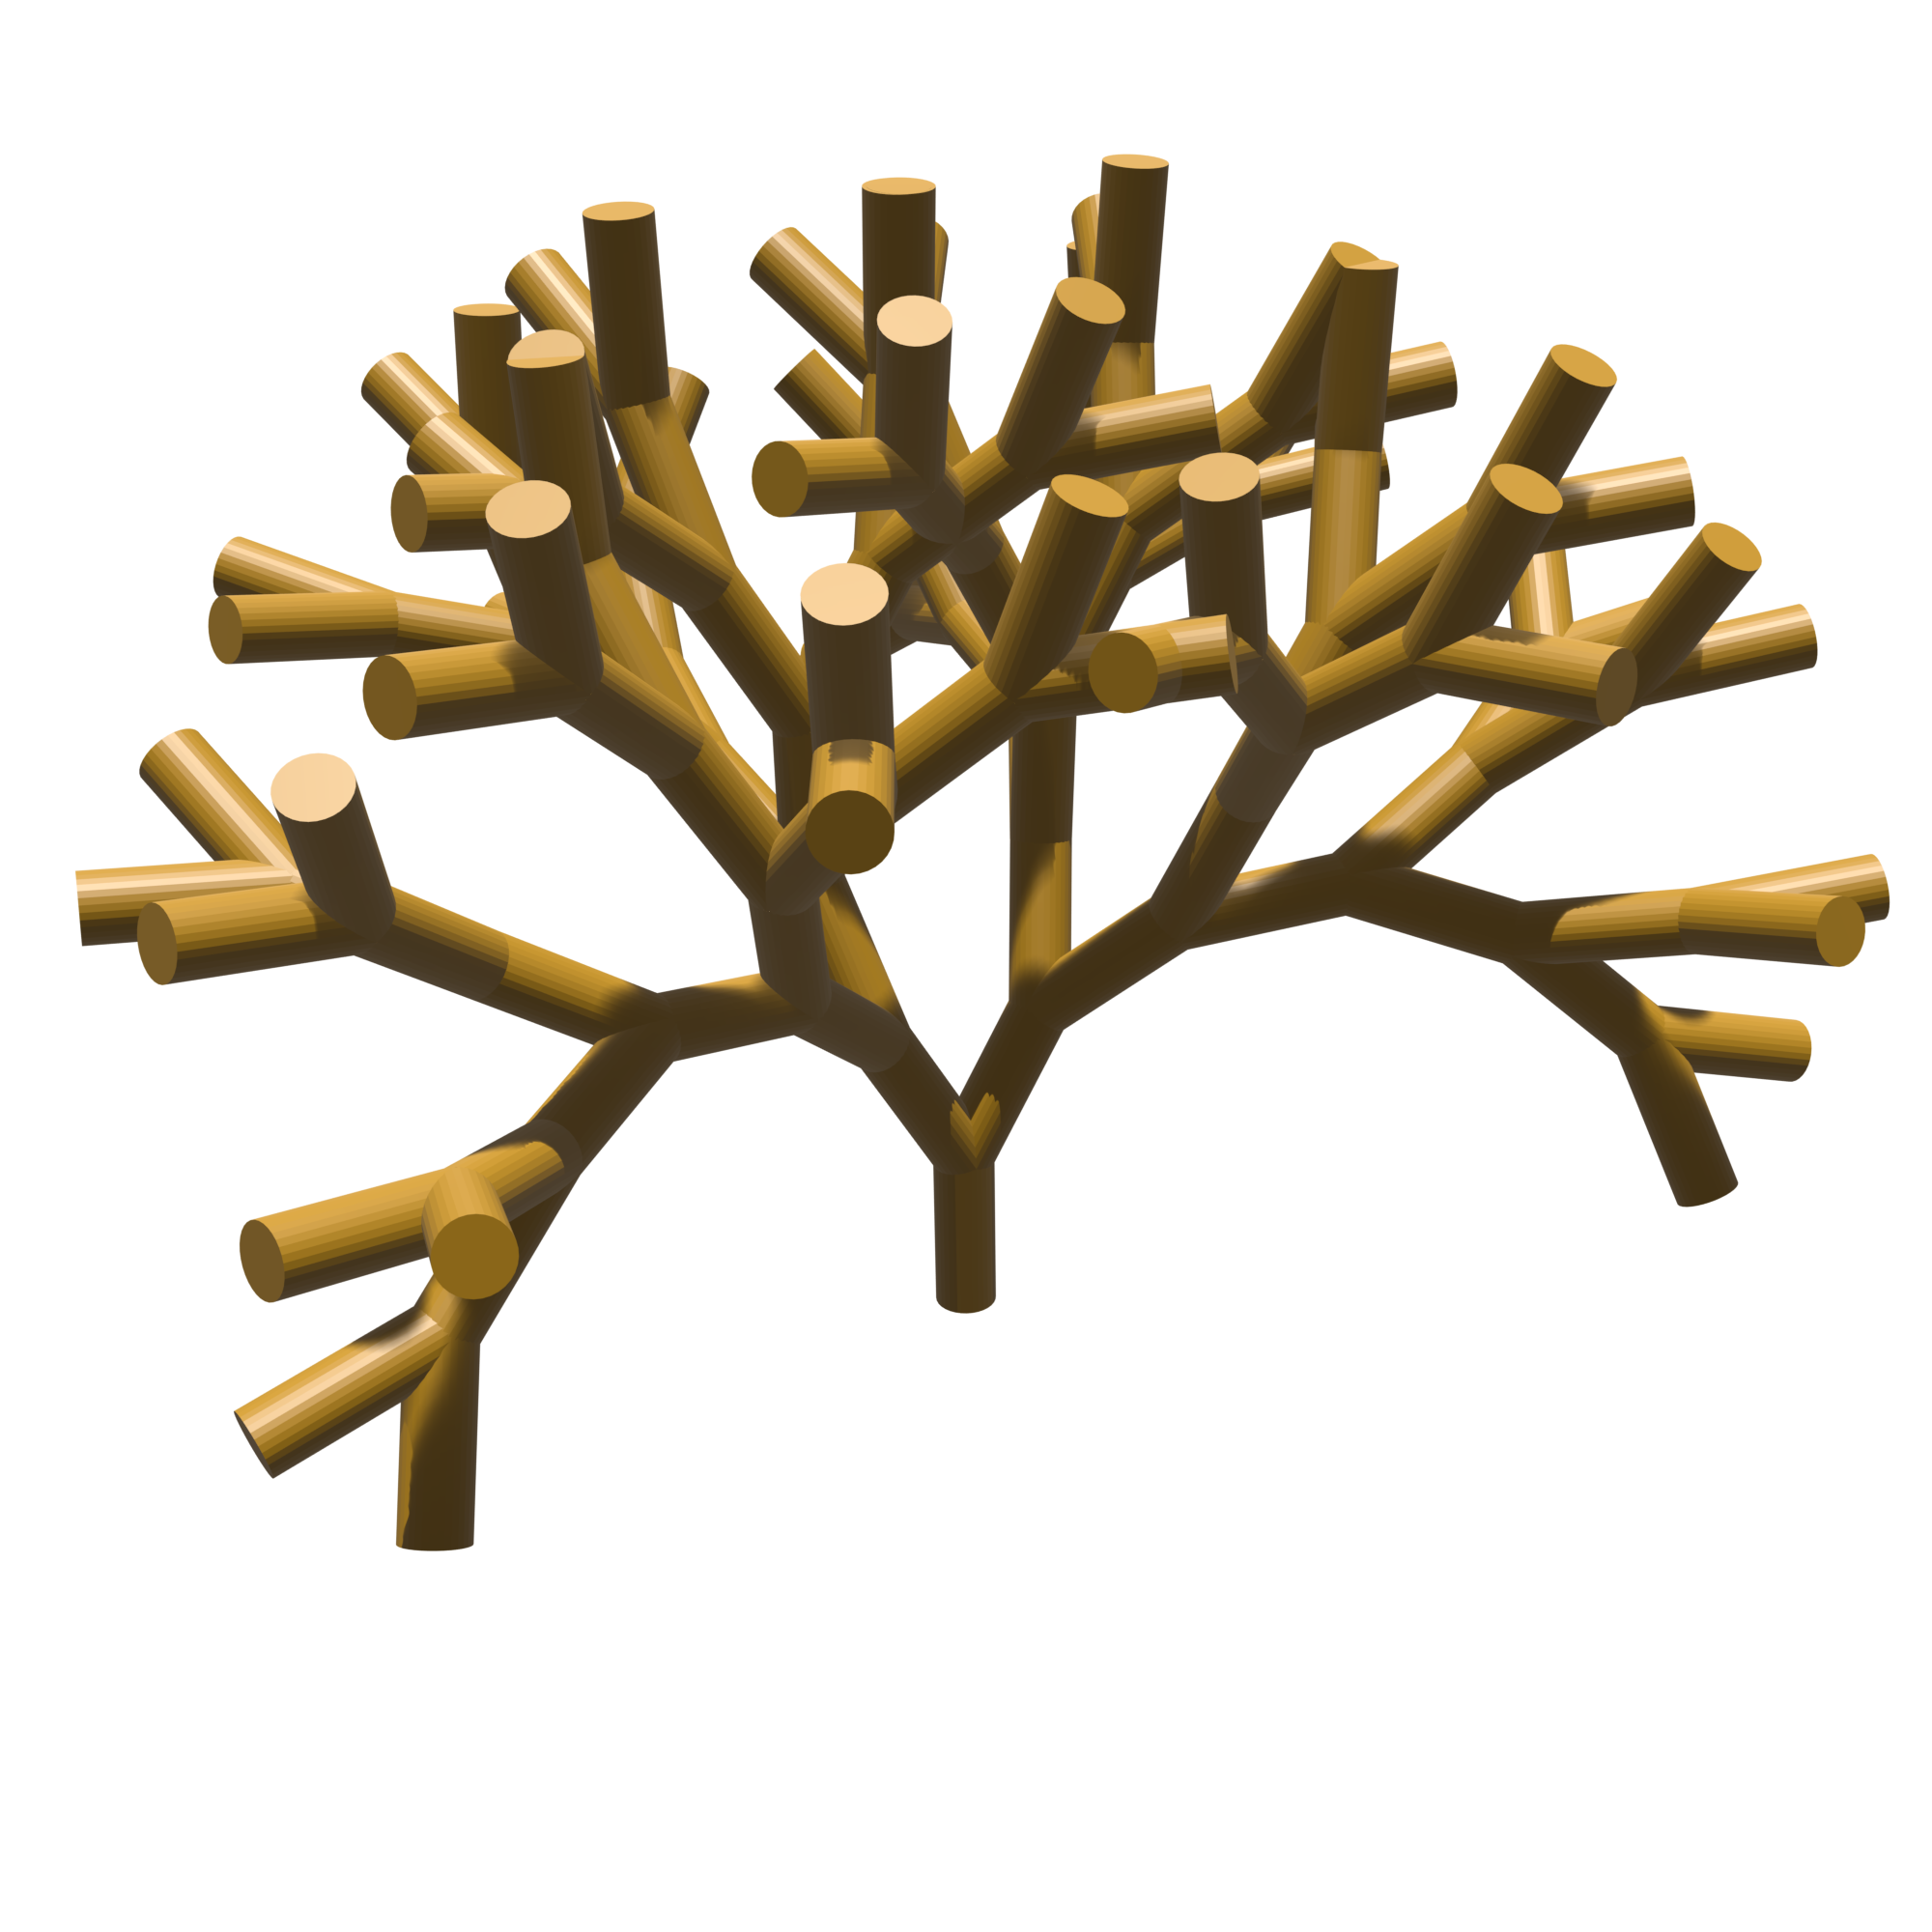
\includegraphics[width=\textwidth]{figures/L-systems/tree1.png}
    \caption{A nice 3D tree}
\end{figure}

\begin{figure}[H]
    \centering
    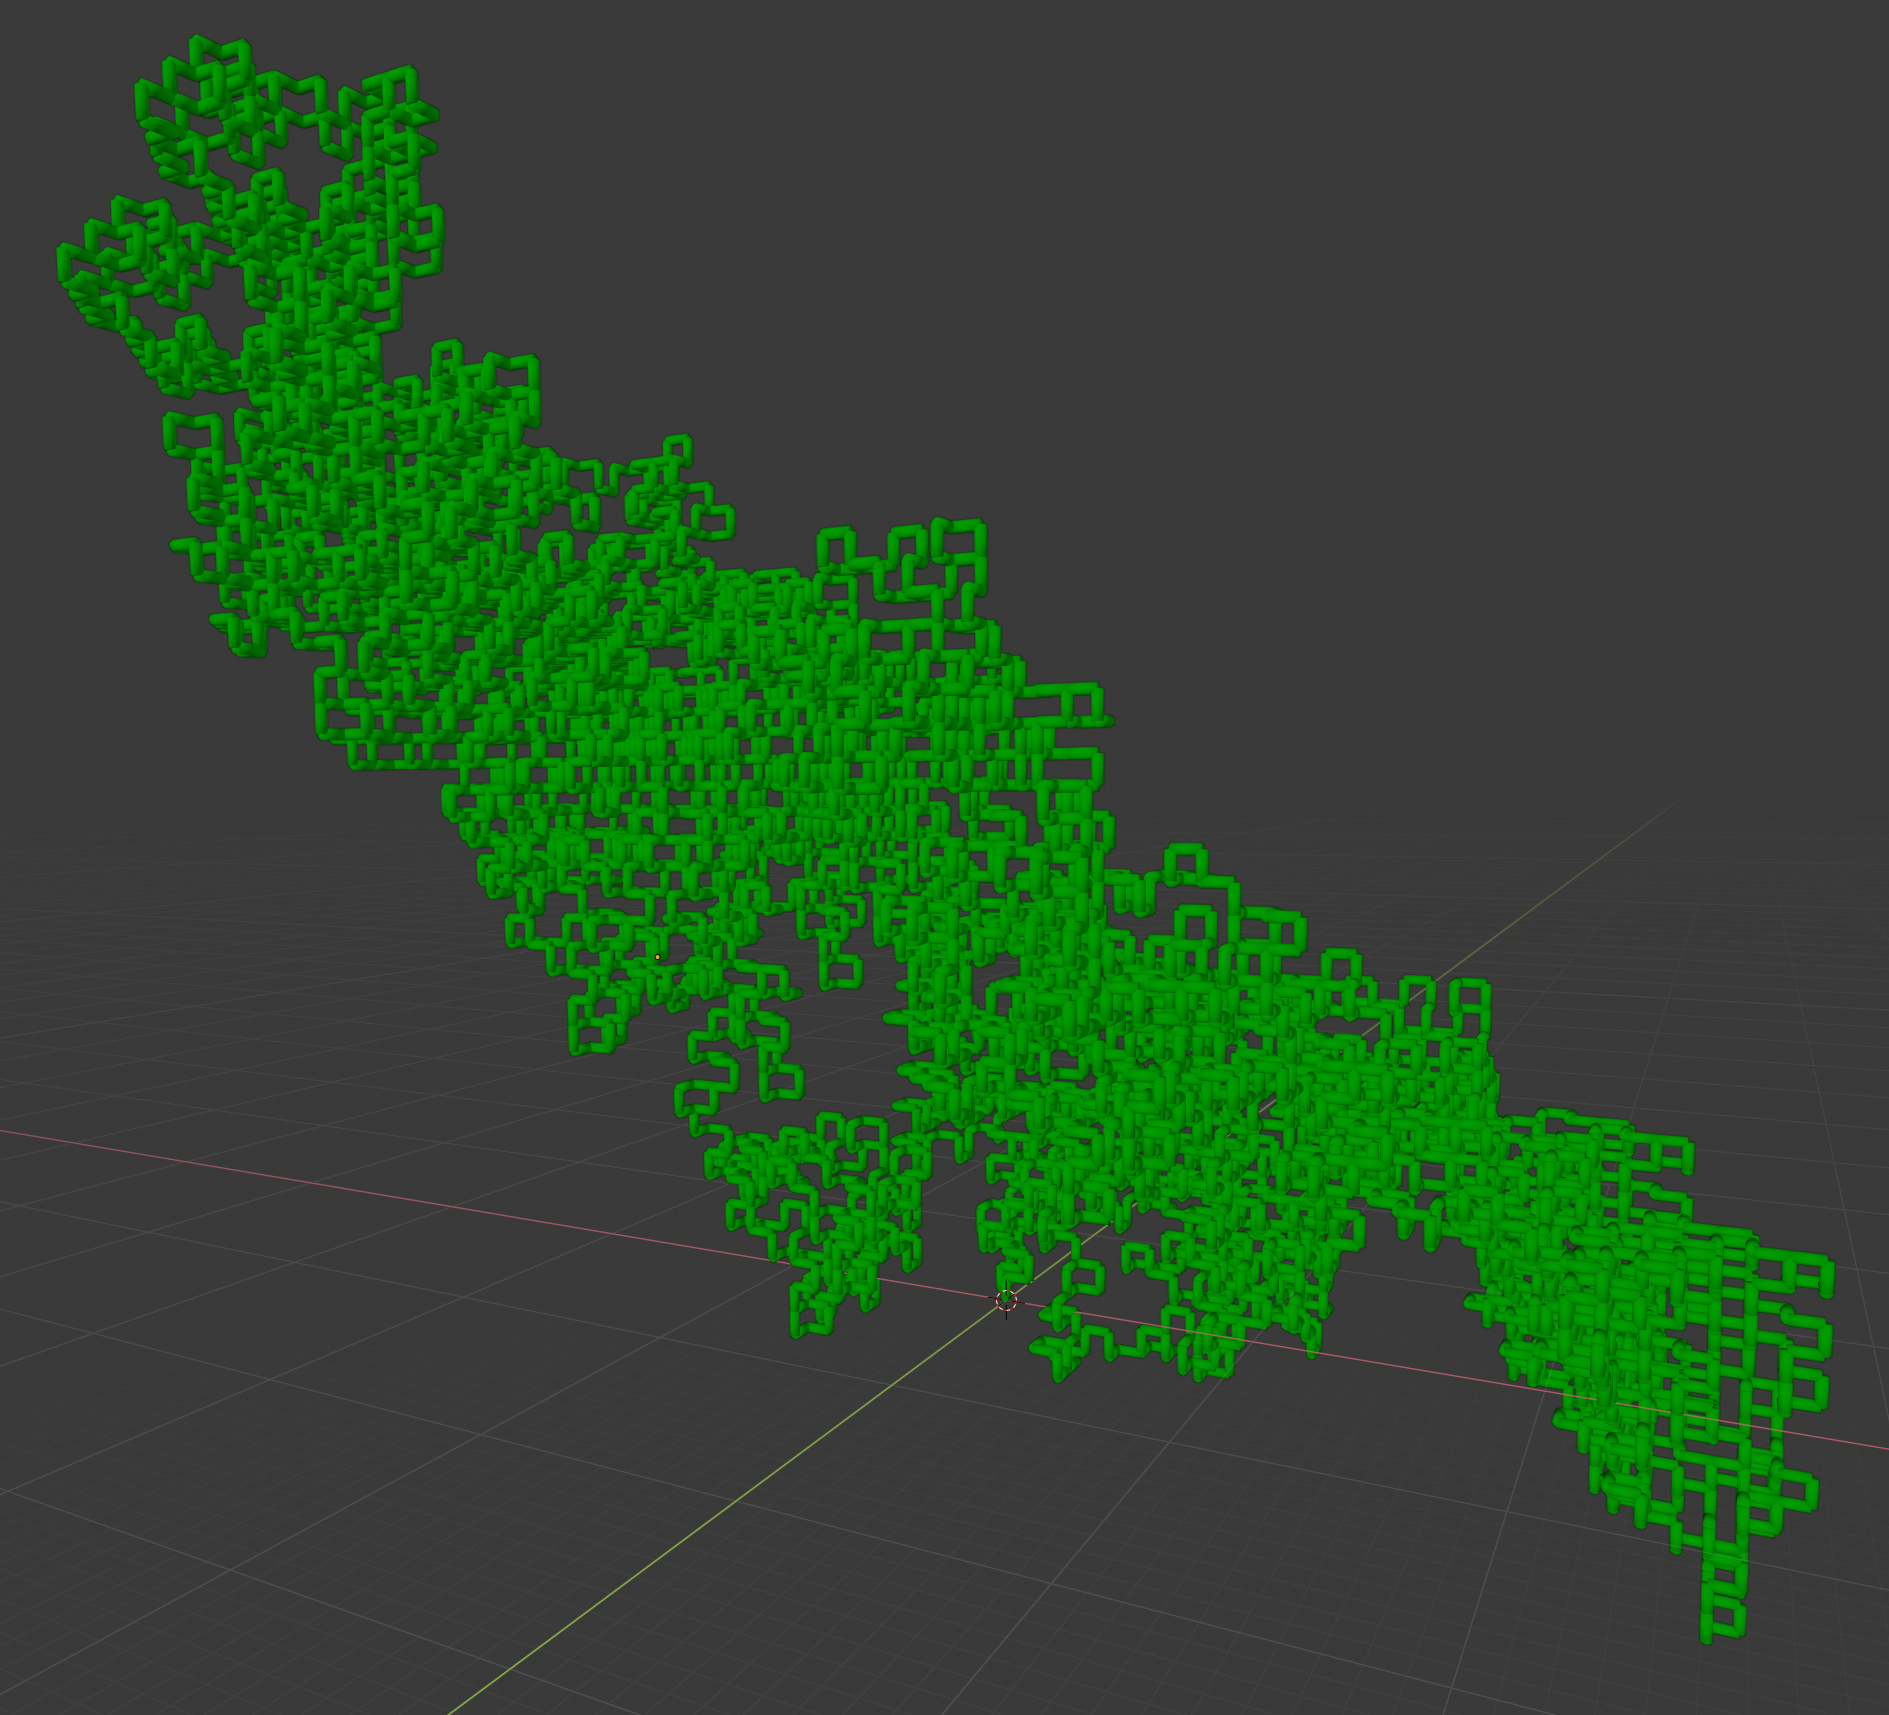
\includegraphics[width=\textwidth]{figures/L-systems/dragon0-3d.png}
    \caption{A 3d variant of the dragon curve}
\end{figure}

\begin{figure}[H]
    \centering
    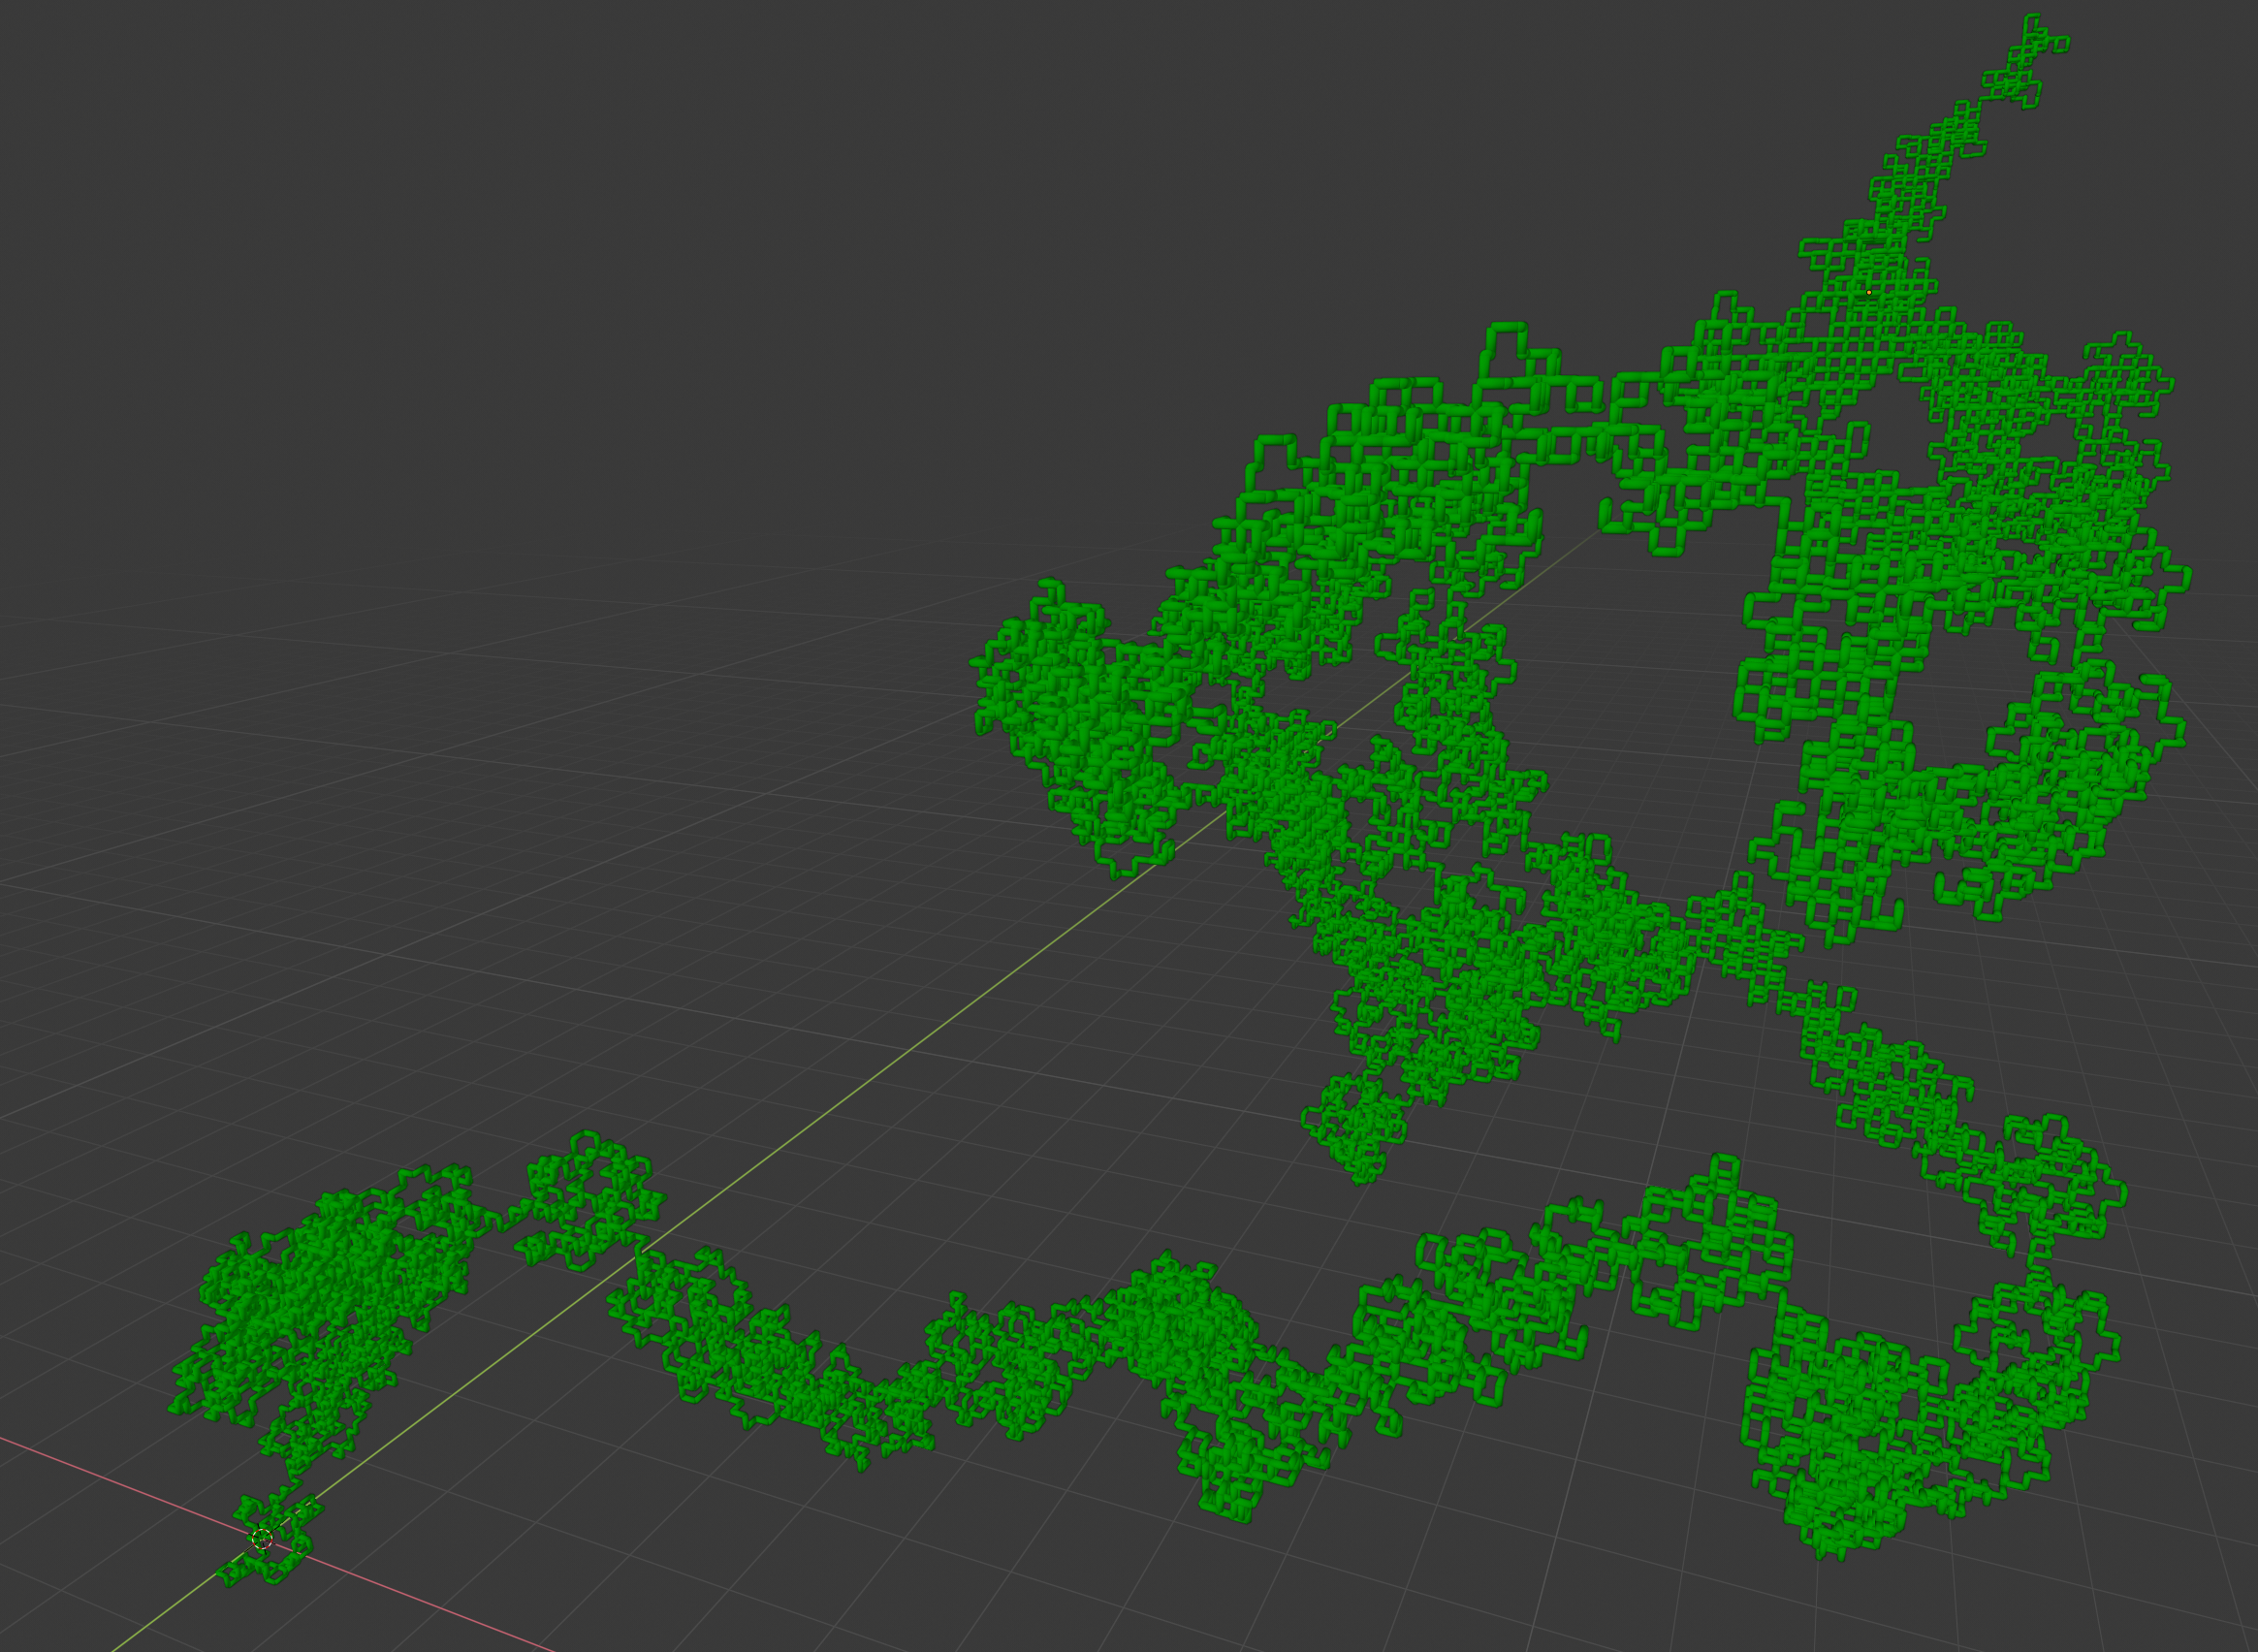
\includegraphics[width=\textwidth]{figures/L-systems/dragon1-3d.png}
    \caption{A 3d variant of the dragon curve}
\end{figure}

\begin{figure}[H]
    \centering
    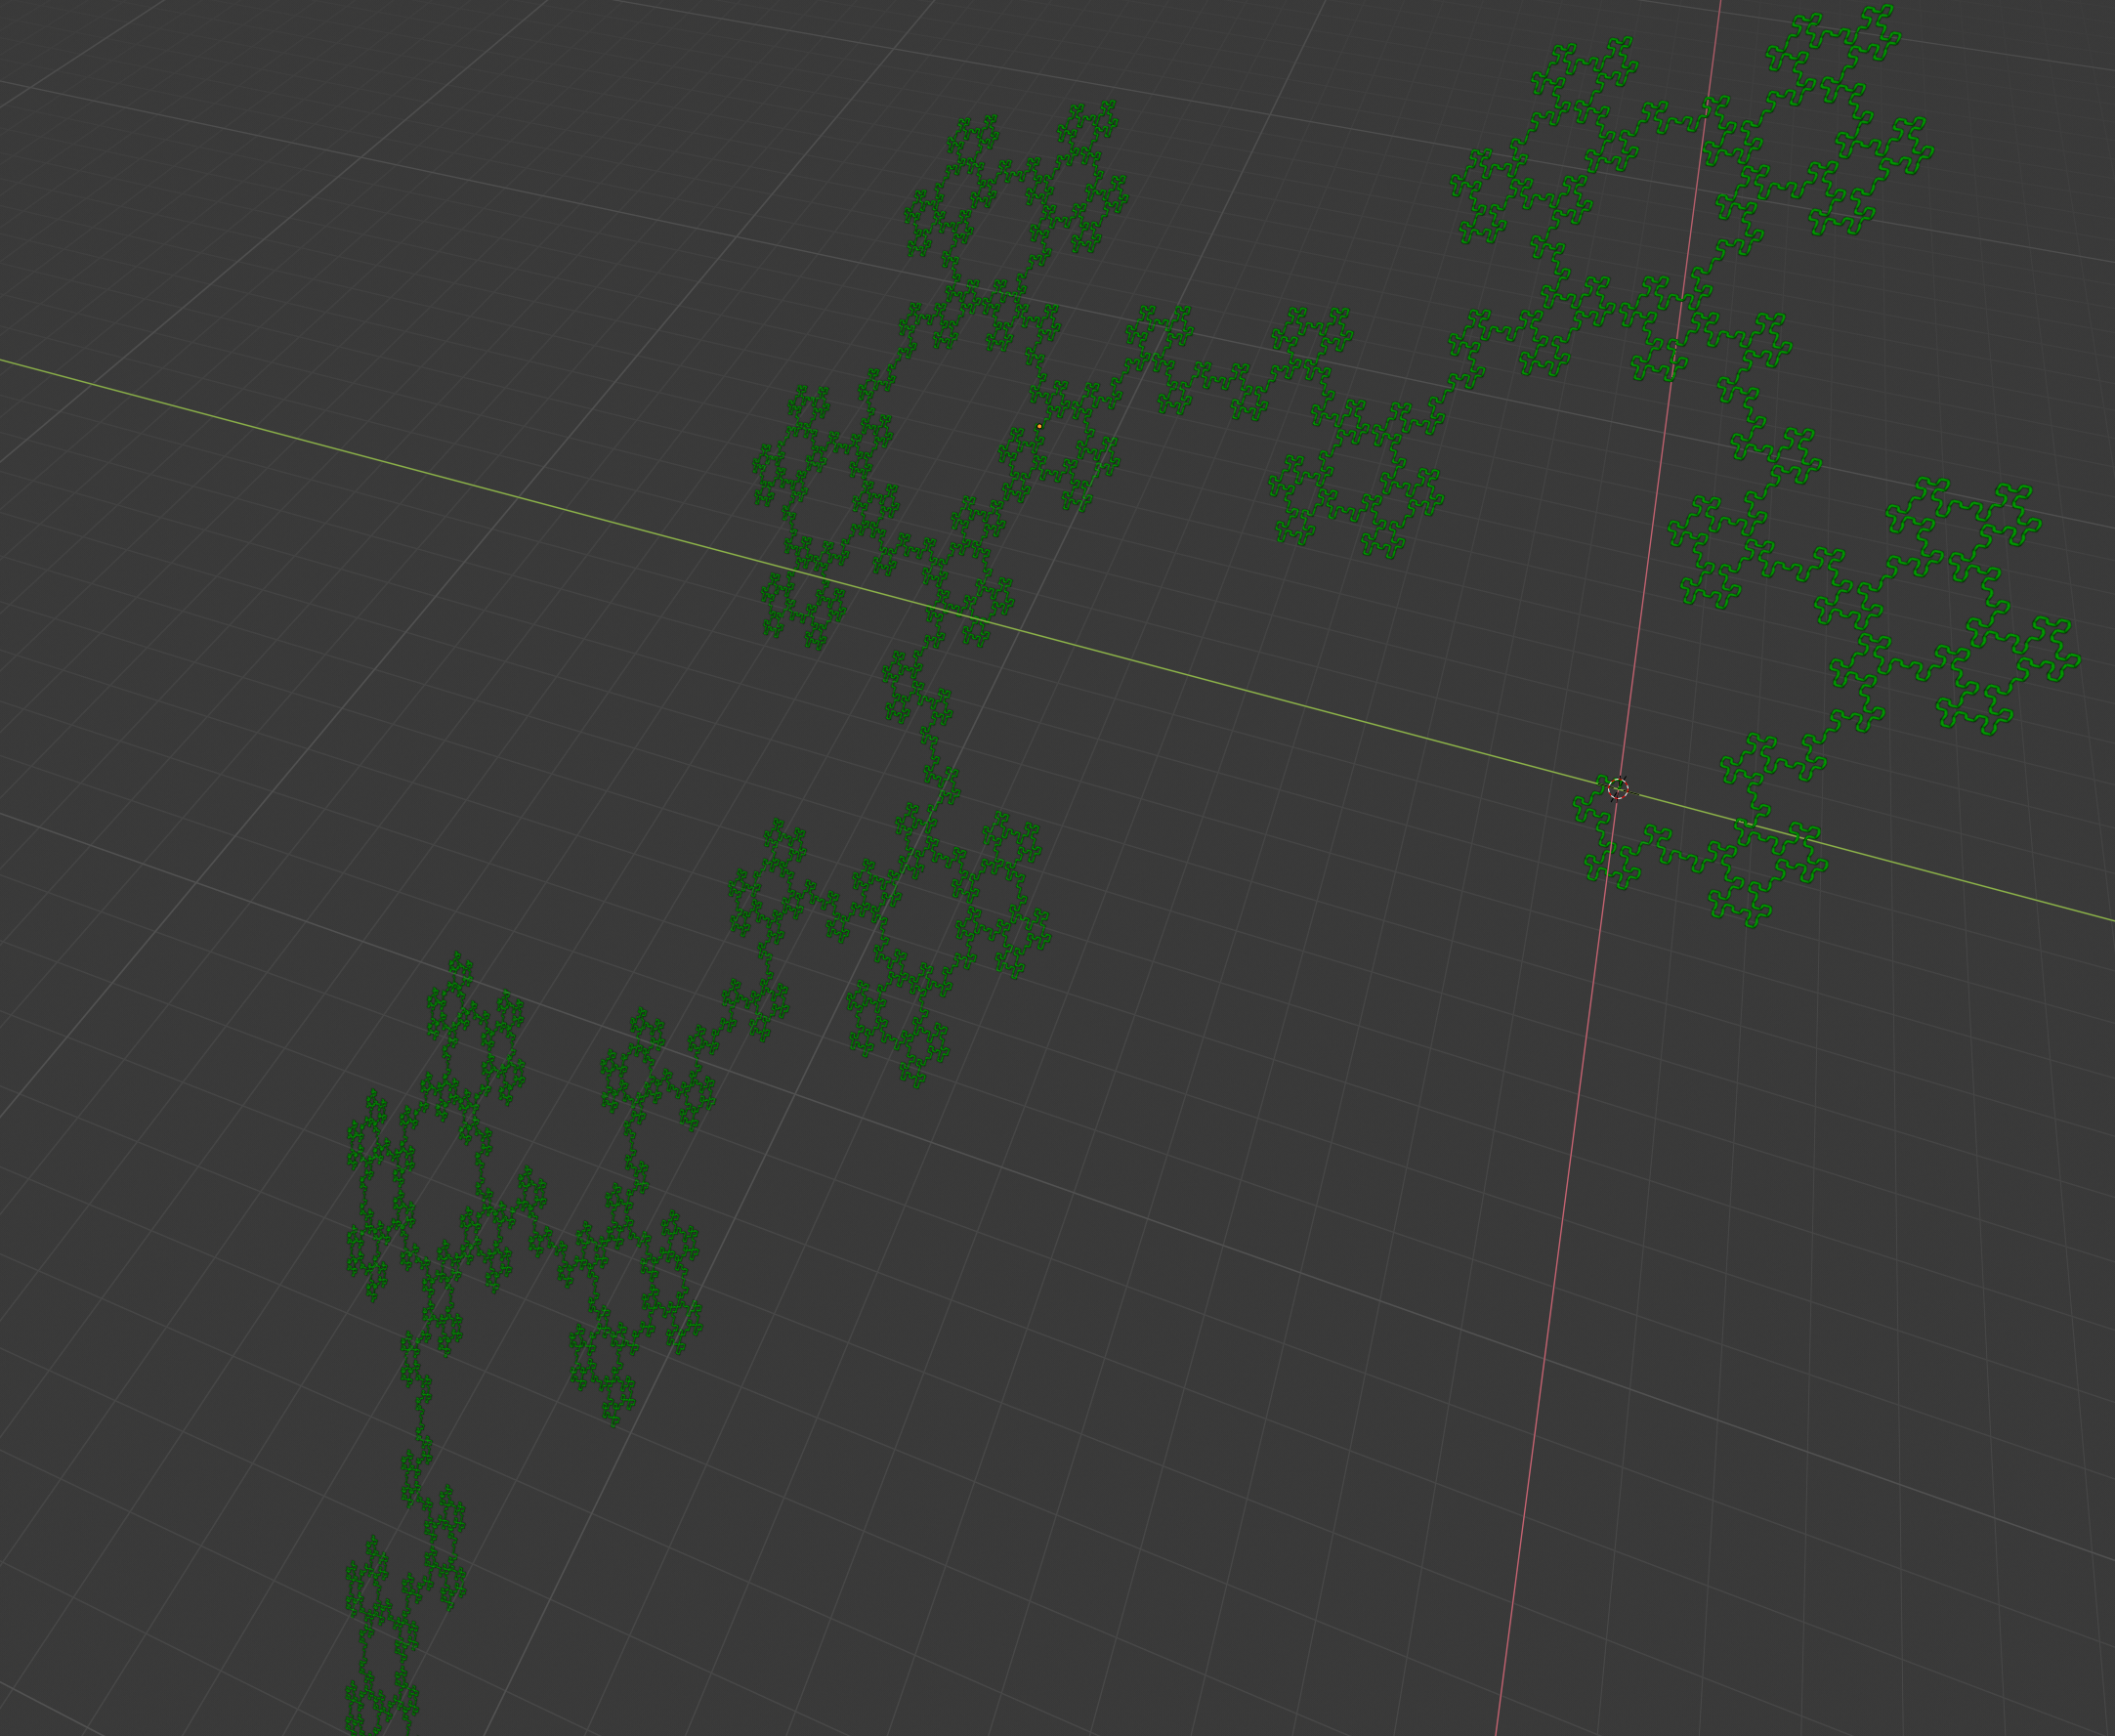
\includegraphics[width=\textwidth]{figures/L-systems/dragon2-3d.png}
    \caption{A 3d variant of the dragon curve}
\end{figure}

\begin{figure}[H]
    \centering
    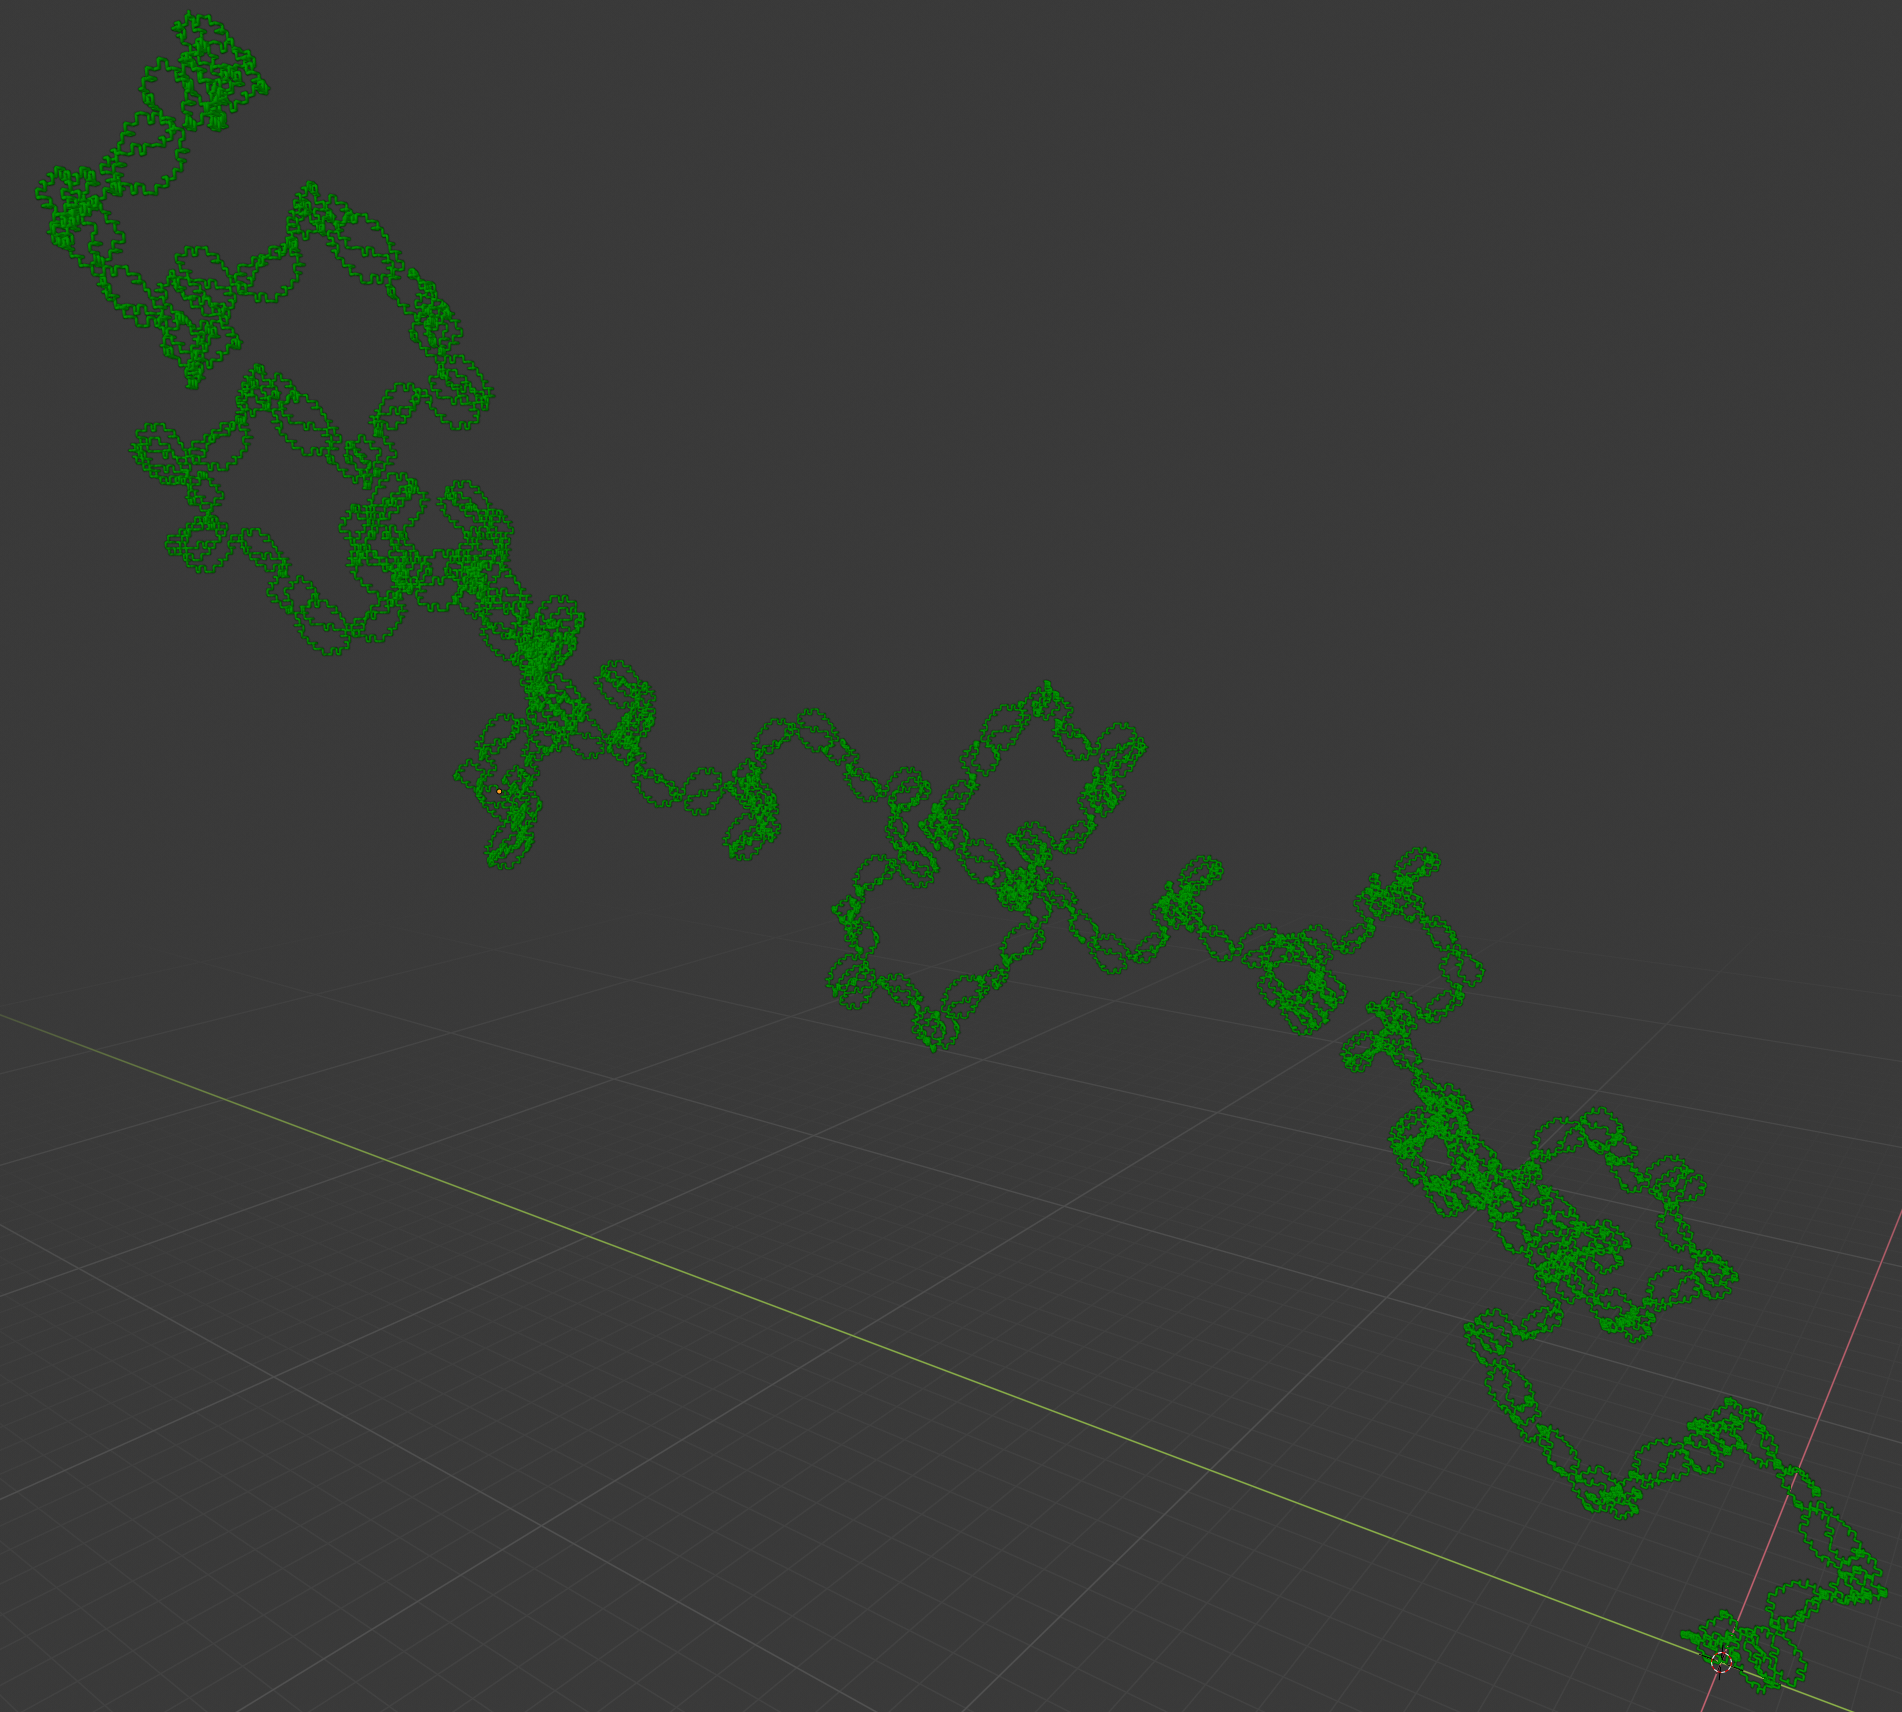
\includegraphics[width=\textwidth]{figures/L-systems/dragon3-3d.png}
    \caption{A 3d variant of the dragon curve}
\end{figure}

\begin{figure}[H]
    \centering
    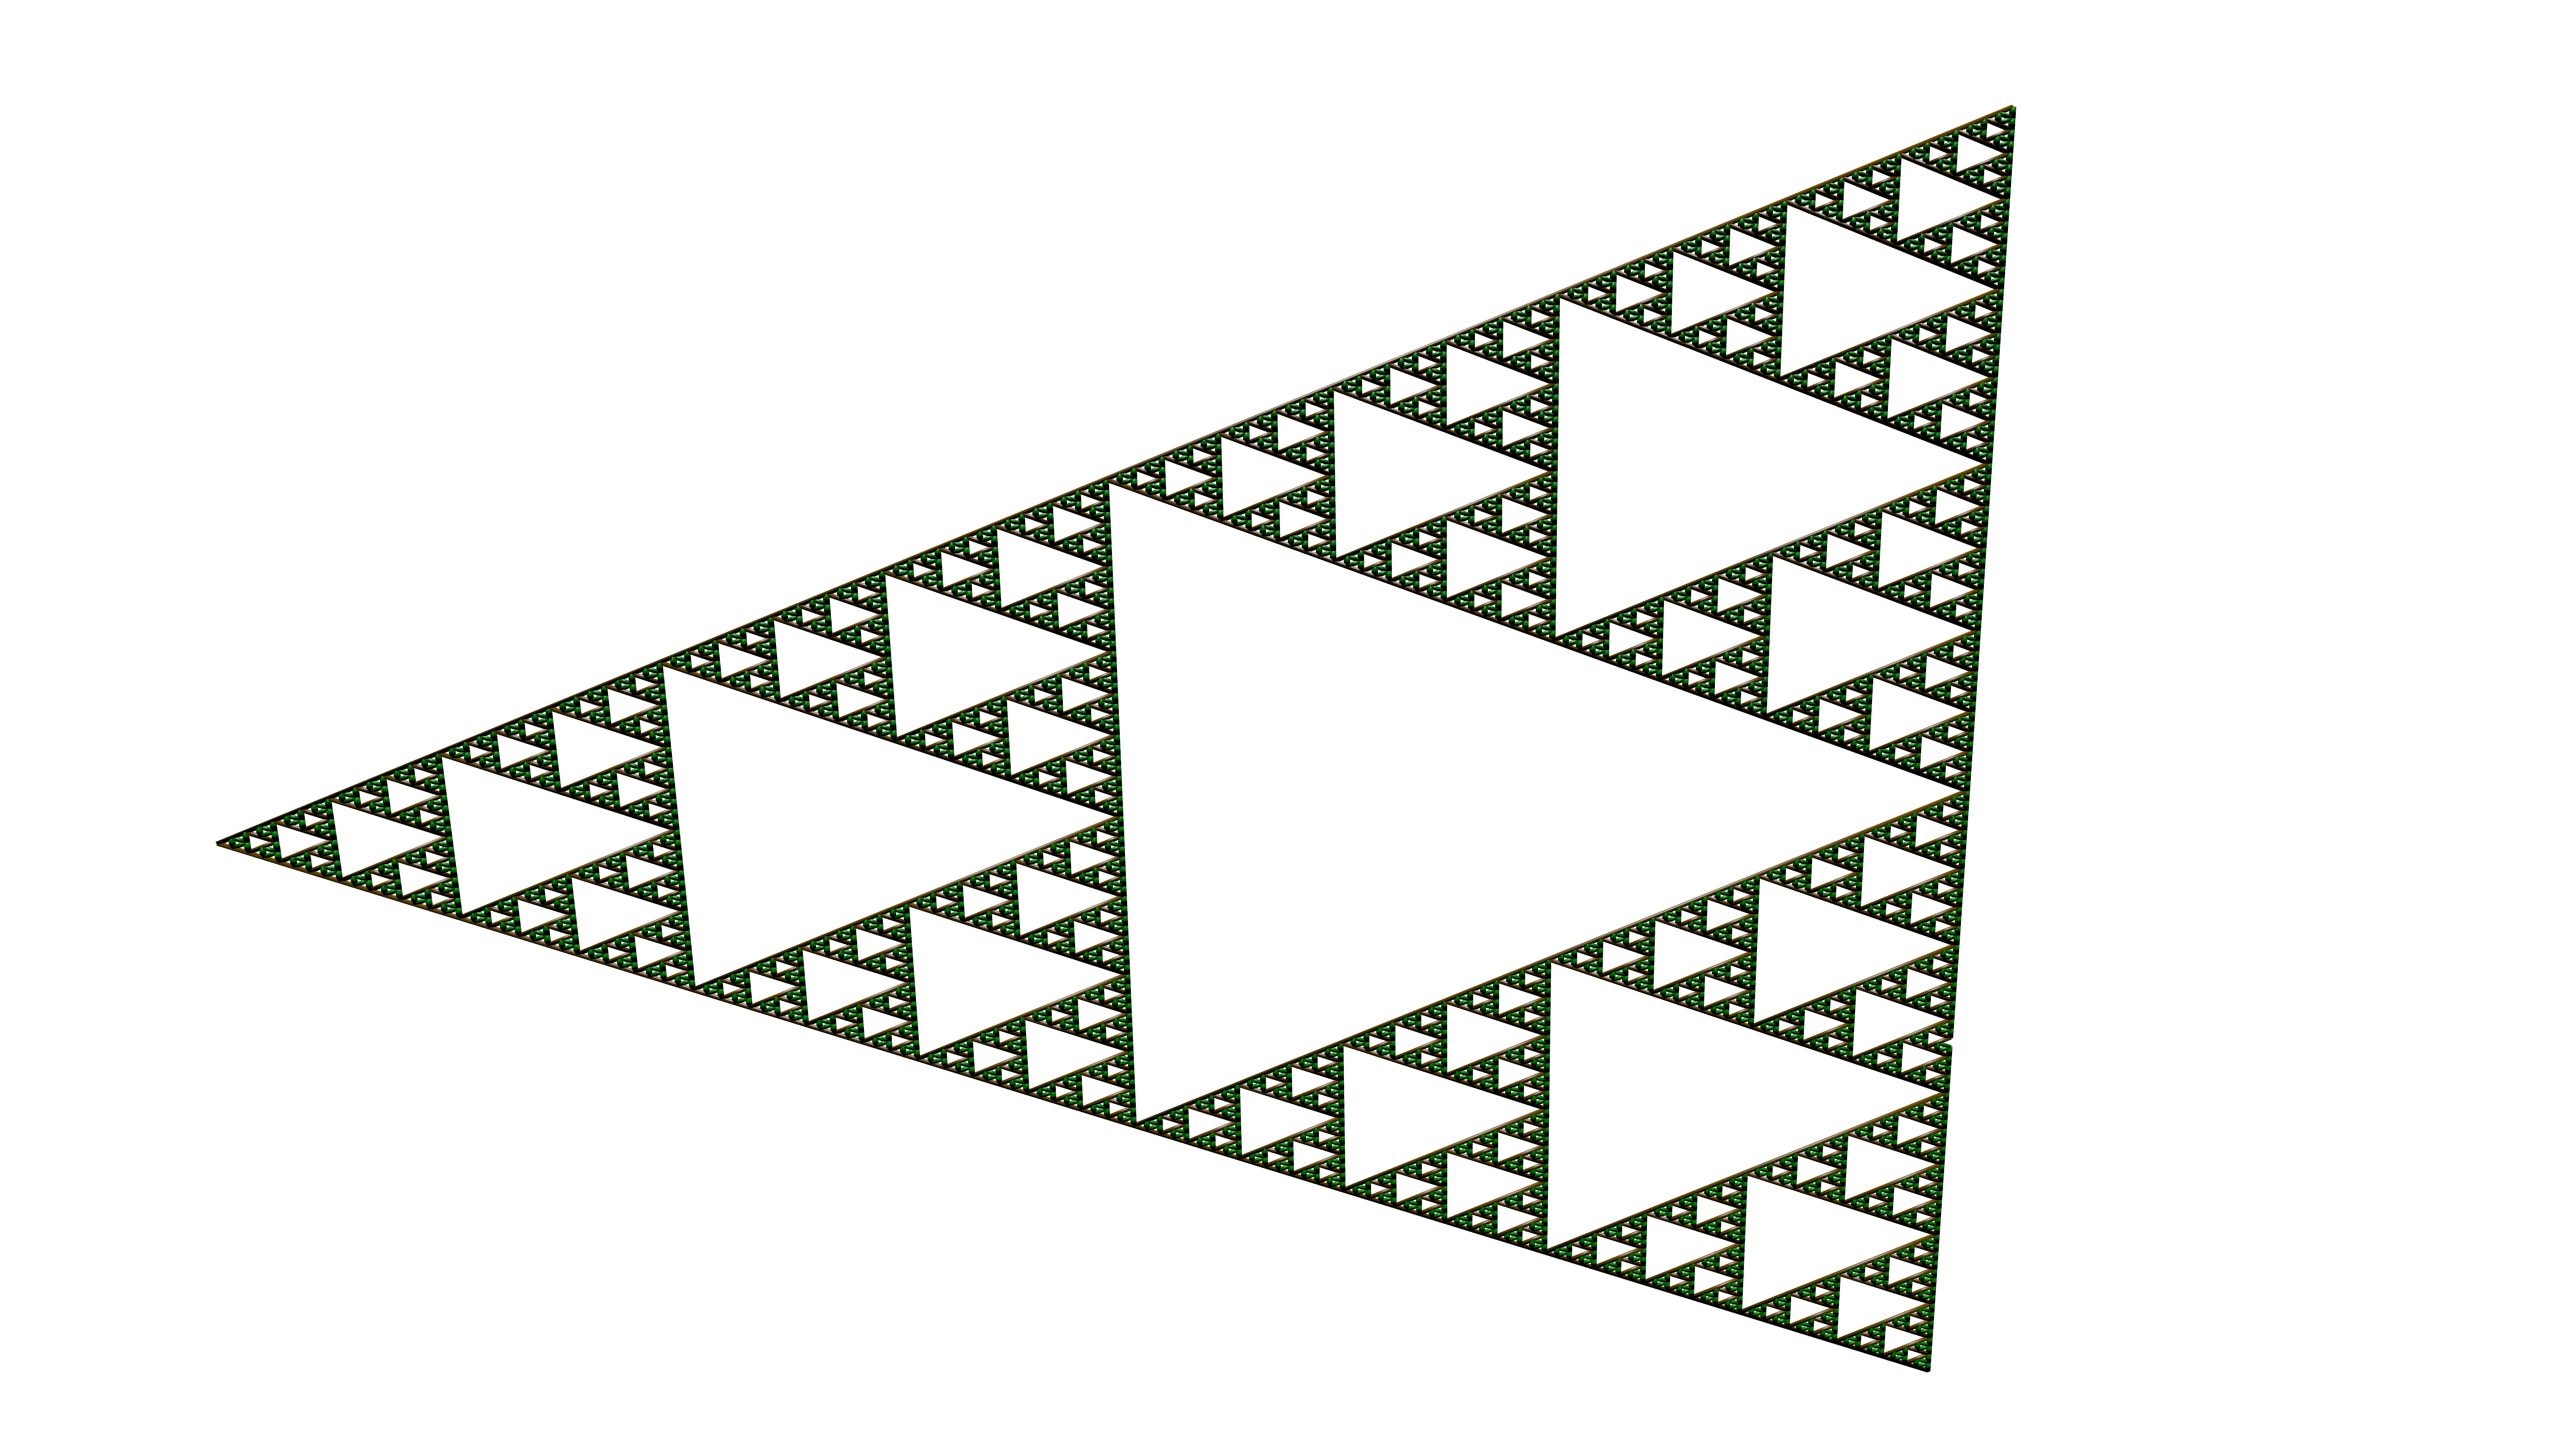
\includegraphics[width=0.90\textwidth]{figures/L-systems/sierpinski.png}
    \caption{Problem 2 Sierpiński Triangle}\label{fig:sierpinski}
\end{figure}

\begin{figure}[H]
    \centering
    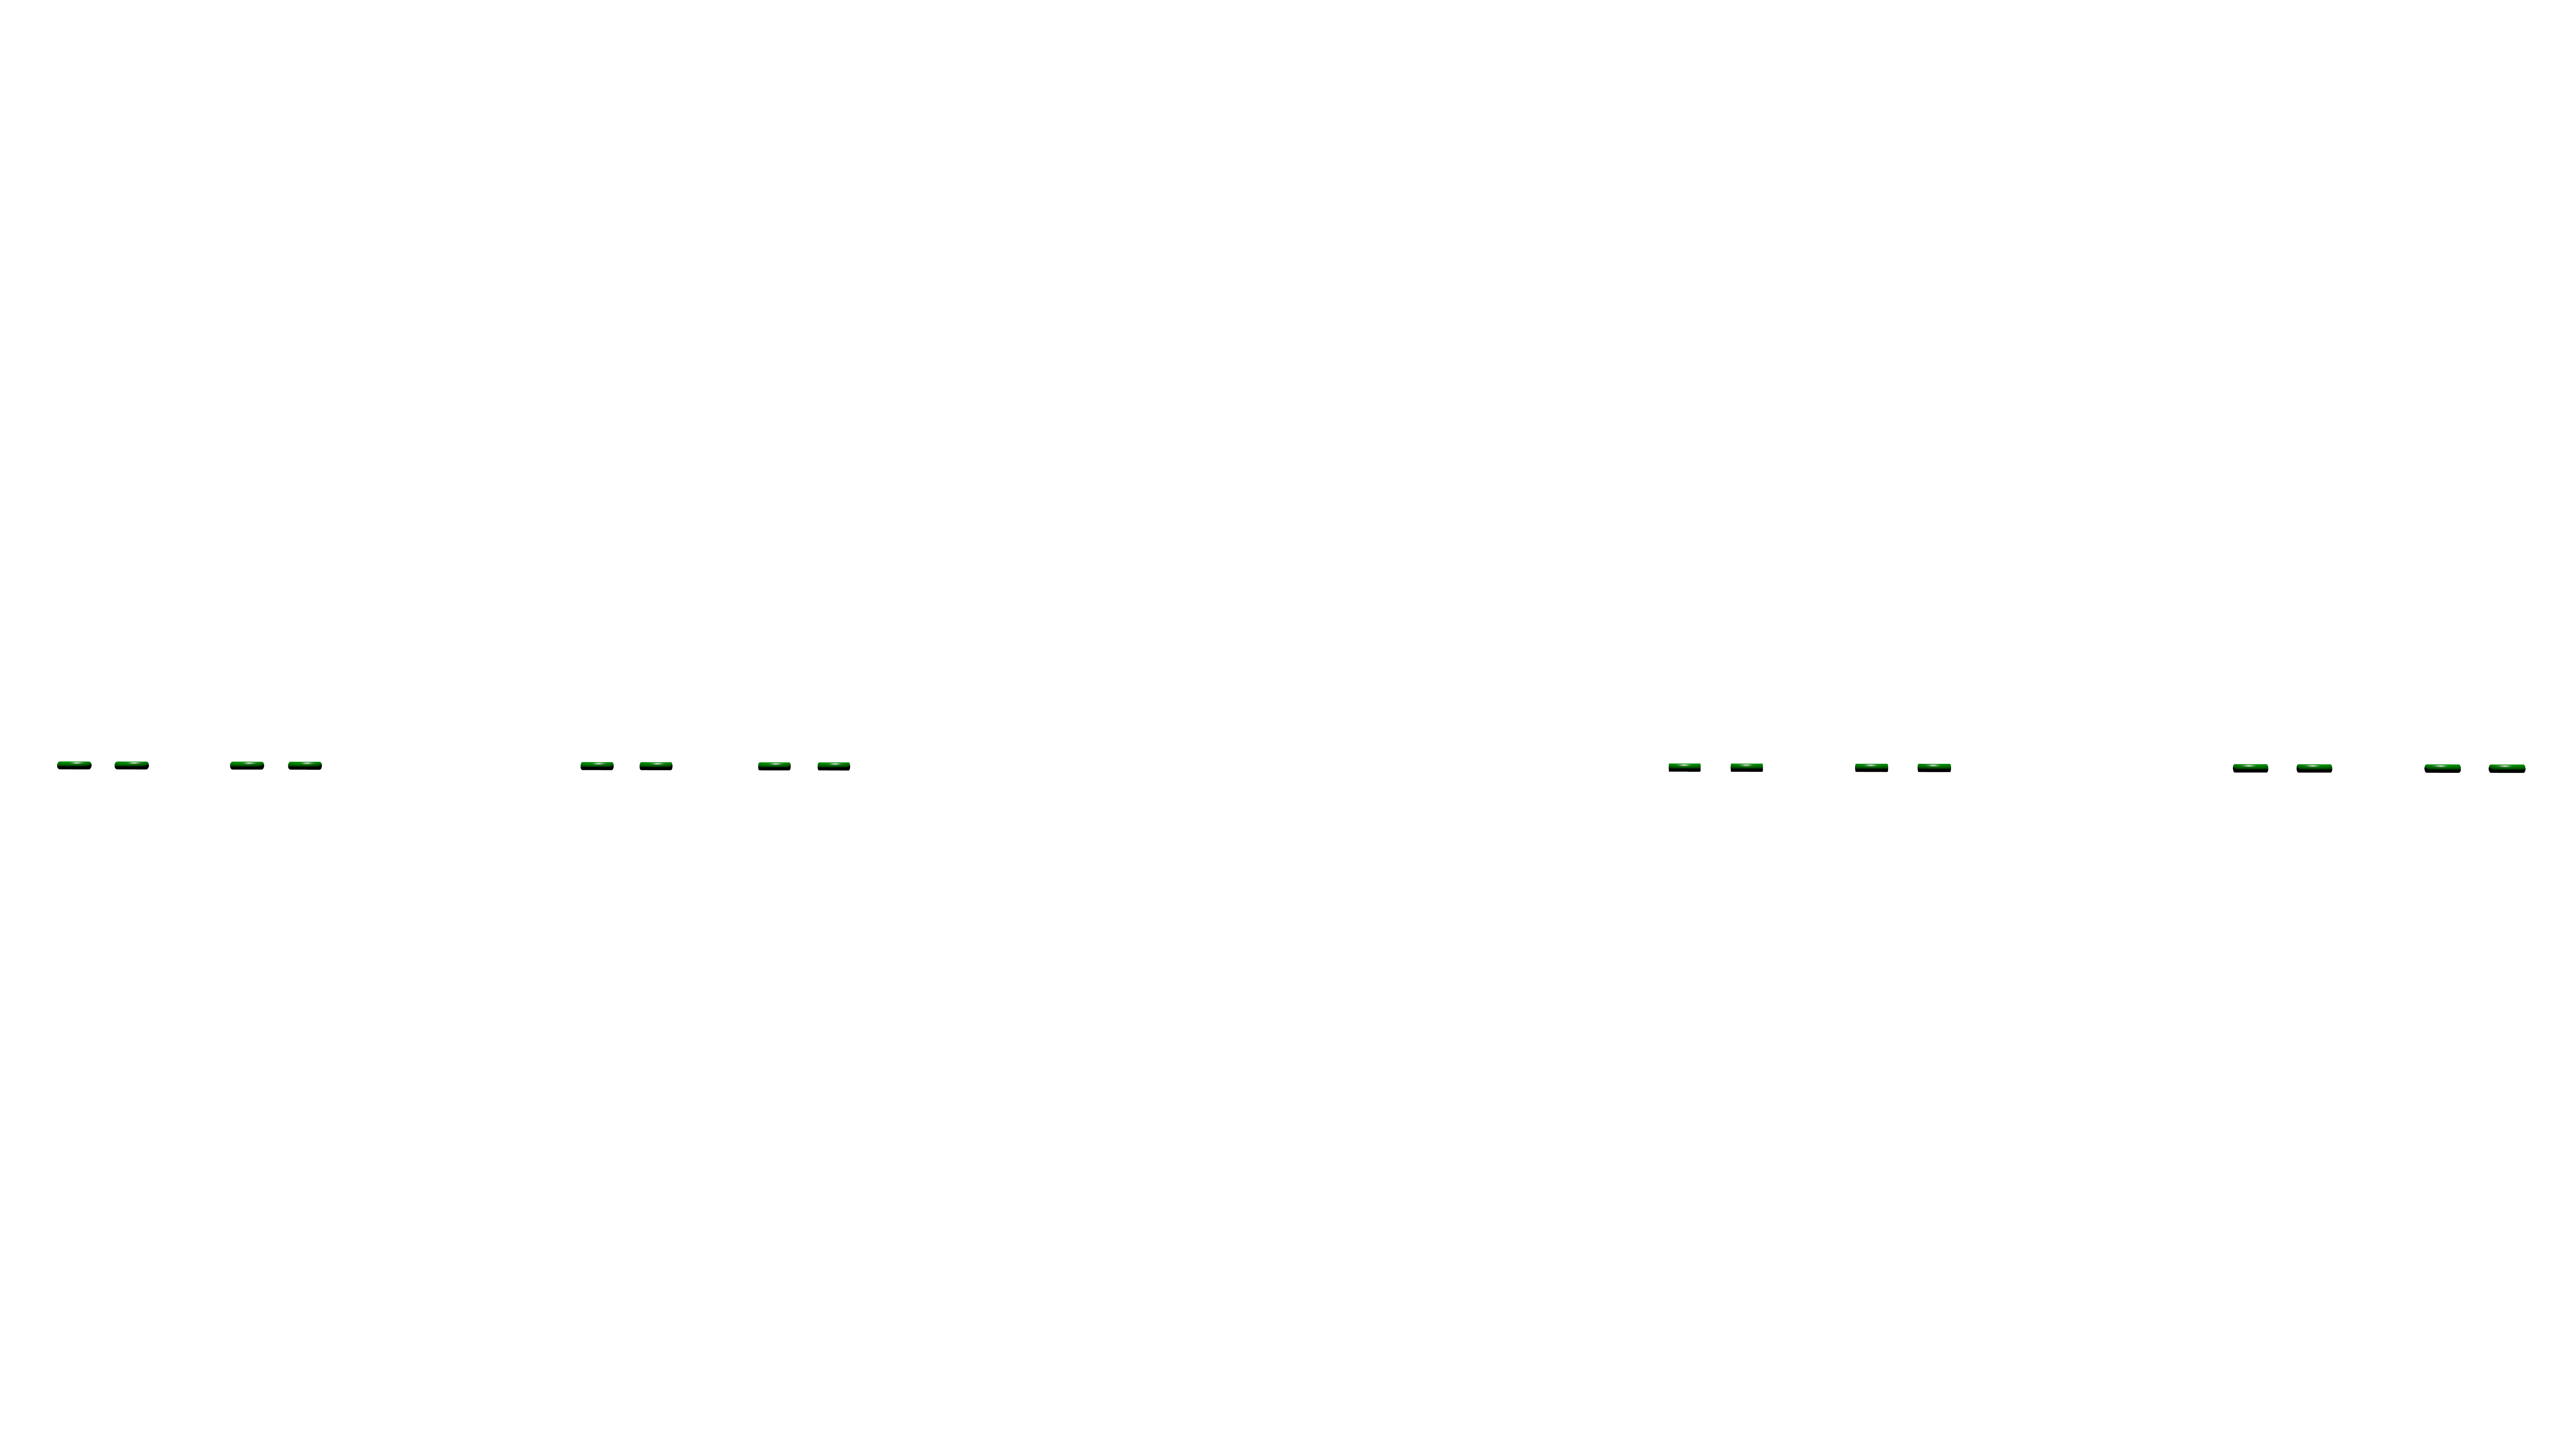
\includegraphics[width=0.70\textwidth]{figures/L-systems/cantor.png}
    \caption{Problem 2 Cantor Set}\label{fig:cantor}
\end{figure}

\begin{figure}[H]
    \centering
    \includegraphics[width=0.90\textwidth]{figures/L-systems/k3d_v4.png}
    \caption{Problem 2 Custom Variant with Proportional Radii Cylinders}\label{fig:k3d_v4}
\end{figure}

\subsection{Conclusion}
The book examples were extremely simple to implement, we simply
created JSON files that matched the book description. To build the 3D
variants we experimented until they looked decent. The other variants were
through trial and error or online examples. It was fun to play with the
different rules and attempt to get structures that were uniform but didn't
entirely look uniform.
